\documentclass[]{scrbook}
\usepackage{lmodern}
\usepackage{amssymb,amsmath}
\usepackage{ifxetex,ifluatex}
\usepackage{fixltx2e} % provides \textsubscript
\ifnum 0\ifxetex 1\fi\ifluatex 1\fi=0 % if pdftex
  \usepackage[T1]{fontenc}
  \usepackage[utf8]{inputenc}
\else % if luatex or xelatex
  \ifxetex
    \usepackage{mathspec}
  \else
    \usepackage{fontspec}
  \fi
  \defaultfontfeatures{Ligatures=TeX,Scale=MatchLowercase}
\fi
% use upquote if available, for straight quotes in verbatim environments
\IfFileExists{upquote.sty}{\usepackage{upquote}}{}
% use microtype if available
\IfFileExists{microtype.sty}{%
\usepackage[]{microtype}
\UseMicrotypeSet[protrusion]{basicmath} % disable protrusion for tt fonts
}{}
\PassOptionsToPackage{hyphens}{url} % url is loaded by hyperref
\usepackage[unicode=true]{hyperref}
\hypersetup{
            pdftitle={Solver for Hydrologic Unstructured Domain (SHUD)},
            pdfauthor={Lele Shu (lele.shu@gmail.com)},
            pdfborder={0 0 0},
            breaklinks=true}
\urlstyle{same}  % don't use monospace font for urls
\usepackage{natbib}
\bibliographystyle{apalike}
\usepackage{longtable,booktabs}
% Fix footnotes in tables (requires footnote package)
\IfFileExists{footnote.sty}{\usepackage{footnote}\makesavenoteenv{long table}}{}
\usepackage{graphicx,grffile}
\makeatletter
\def\maxwidth{\ifdim\Gin@nat@width>\linewidth\linewidth\else\Gin@nat@width\fi}
\def\maxheight{\ifdim\Gin@nat@height>\textheight\textheight\else\Gin@nat@height\fi}
\makeatother
% Scale images if necessary, so that they will not overflow the page
% margins by default, and it is still possible to overwrite the defaults
% using explicit options in \includegraphics[width, height, ...]{}
\setkeys{Gin}{width=\maxwidth,height=\maxheight,keepaspectratio}
\IfFileExists{parskip.sty}{%
\usepackage{parskip}
}{% else
\setlength{\parindent}{0pt}
\setlength{\parskip}{6pt plus 2pt minus 1pt}
}
\setlength{\emergencystretch}{3em}  % prevent overfull lines
\providecommand{\tightlist}{%
  \setlength{\itemsep}{0pt}\setlength{\parskip}{0pt}}
\setcounter{secnumdepth}{5}
% Redefines (sub)paragraphs to behave more like sections
\ifx\paragraph\undefined\else
\let\oldparagraph\paragraph
\renewcommand{\paragraph}[1]{\oldparagraph{#1}\mbox{}}
\fi
\ifx\subparagraph\undefined\else
\let\oldsubparagraph\subparagraph
\renewcommand{\subparagraph}[1]{\oldsubparagraph{#1}\mbox{}}
\fi

% set default figure placement to htbp
\makeatletter
\def\fps@figure{htbp}
\makeatother

\usepackage{booktabs}

\title{Solver for Hydrologic Unstructured Domain (SHUD)}
\providecommand{\subtitle}[1]{}
\subtitle{User Guide}
\author{Lele Shu
(\href{mailto:lele.shu@gmail.com}{\nolinkurl{lele.shu@gmail.com}})}
\date{2019-12-22}

\begin{document}
\maketitle

{
\setcounter{tocdepth}{2}
\tableofcontents
}
\chapter{Overview}\label{Overview}

This file is a user guide or technical documentation of the SHUD
modeling system. PDF version of the User Guide is available via
:\href{https://www.shud.xyz/_book/SHUD_User_Guide.pdf}{SHUD User Guide}

The Solver for Hydrologic Unstructured Domain (SHUD - pronounced
``SHOULD'') is a multi-process, multi-scale hydrological model where
major hydrological processes are fully coupled using the semi-discrete
\textbf{Finite Volume Method} (FVM).

\textbf{SHUDtoolbox} is an open-source GIS and hydrological analysis
toolbox designed for the SHUD modeling system. The SHUDtoolbox provides
access to the digital data sets (terrain, forcing, and parameters) and
tools necessary to drive the model, as well as a collection of GIS-based
pre- and post-processing tools.

Collectively the system is referred to as the \textbf{SHUD Modeling
System}.

The SHUD and SHUDtoolbox is an open-source software, freely available
for download at \href{https://SHUD-system.github.io}{SHUD website} or
\href{https://github.com/SHUD-System/}{Github Page} along with
installation and user guides.

\section{Standing on the shoulders of
giants}\label{standing-on-the-shoulders-of-giants}

As a descendant of PIHM, SHUD inherits the fundamental idea of solving
hydrological variables in CVODE. The code has been completely rewritten
in a new programming language, with a new discretization and
corresponding improvements to the underlying algorithms, adapting new
mathematical schemes and a new user-friendly input/output data format.
Although SHUD is forked from PIHM's track, SHUD still inherits the use
of CVODE for solving the ODEs but modernizes and extends PIHM's
technical and scientific capabilities. The SHUD is imcompatible to PIHM.

It is our intention (me and previous PIHM group)to begin a debate on the
role of \emph{Community Models} in the hydrologic sciences.

SHUD and PIHM represent our strategy for the synthesis of
\emph{multi-state}, \emph{multi-scale} distributed hydrologic models
using the integral representation of the underlying physical process
equations and state variables.

Our interest is in devising a concise representation of watershed and/or
river basin hydrodynamics, which allows interactions among major
physical processes operating simultaneously, but with the flexibility to
add or eliminate states/processes/constitutive relations depending on
the objective of the numerical experiment or purpose of the scientific
or operational application.

To satisfy the objectives, the SHUD\ldots{}

\begin{itemize}
\tightlist
\item
  is a distributed hydrologic model, based on the semi-discrete
  \textbf{Finite Volume Method (FVM)} in which domain discretization is
  an unstructured triangular irregular network (e.g.~Delaunay triangles)
  generated with constraints (geometric, and parametric). A local
  prismatic control volume is formed by the vertical projection of the
  Delaunay triangles forming each layer of the model. Given a set of
  constraints (e.g.~river network support, watershed boundary, altitude
  zones, ecological regions, hydraulic properties, climate zones, etc),
  an ``optimal'' mesh is generated. River volume cells are also
  prismatic, with trapezoidal or rectangular cross-section, and are
  generated along or cross edges of Delaunay triangles. The local
  control volume contains all equations to be solved and is referred to
  as the model kernel.
\item
  is a physically-based model in which all equations used are describing
  the physics of the hydrological processes which control the catchment.
  The physical model is able to predict the water in the ungage water
  system, to estimate the sediment, pollutants, and vegetation, etc.,
  such that it is practical to be coupled with biochemistry,
  geomorphology, limnology, and other water-related research. The global
  ODE system is assembled by combining all local ODE systems throughout
  the domain and then solved by a state-of-the-art parallel ODE solver
  known as CVODE developed at the Lawrence Livermore National
  Laboratory.
\item
  is a fully-coupled hydrologic model, where the state and flux
  variables in the hydrologic system are solved within the same time
  step and conserve the mass. The fluxes are infiltration, overland
  flow, groundwater recharge, lateral groundwater flow, exchange of
  river and soil/groundwater and river discharge.
\item
  is of an adaptable temporal and spatial resolution. The spatial
  resolution of the model varies from meters to kilometers based
  requirement of modeling and computing resources. The internal time
  step of the iteration step is adjustable; it is able to export the
  status of the catchment in less 1 second to days. Also, the time
  interval for exporting results is configured flexibly. The flexible
  spatial and temporal resolution is rather valuable for community model
  coupling.
\item
  is an open-source model; anyone can access the source code, use and
  submit their improvement.
\item
  is a long-term yield and single-event flood model.
\end{itemize}

\section{Brief History of PIHM
system}\label{brief-history-of-pihm-system}

\begin{itemize}
\tightlist
\item
  2005 PIHM v1.0
\end{itemize}

Dr.~Yizhong Qu \citep{Qu2007} developed and verified the first version
of PIHM in 2001-2005 during his Ph.D.~in Pennsylvania State Unversity,
following the blueprint of Freeze and Harlan (1969). This version of
PIHM is the soul of the PIHM model.

\begin{itemize}
\tightlist
\item
  2009 PIHMgis
\end{itemize}

Dr.~Gopal Bhartt \citep{Bhatt2012} developed the PIHMgis with support of
C++, Qt GUI library, TRIANGLE library, and QGIS developing kit. The
development of PIHMgis makes the learning curve of PIHM moderate and
benefits the developing, modeling and coupling.

\begin{itemize}
\tightlist
\item
  2015 MM-PIHM
\end{itemize}

Dr.~Yuninh Shi led and developed the MM-PIHM (Multi-Module PIHM), which
embedded all modules from PIHM family, such as RT-PIHM, LE-PIHM,
flux-PIHM, BGC-PIHM, etc. together. The sophisticated design and
coupling of the MM-PIHM is the summit of the PIHM as a \emph{Community
Model} that combined all water-related modules together.

\begin{itemize}
\tightlist
\item
  2019 SHUD
\end{itemize}

Based on the accumulated contribution of PIHM modeling and coupling with
related researches, it is necessary to solve the known bugs and
limitations, improve the performance of the model with parallel methods,
and adopt new updates from SUNDIALS solver and programming strategy.

Several publications that may helps:

\begin{itemize}
\tightlist
\item
  \citep{Qu2004}
\item
  \citep{Qu2007}
\item
  \citep{Li2008}
\item
  \citep{Kumar2004a}
\item
  \citep{Kumar2009d}
\item
  \citep{Yu2015}
\item
  \citep{Yu2014}
\item
  \citep{Li2011}
\item
  \citep{Shi2015}
\item
  \citep{Shi2015a}
\item
  \citep{Bhatt2014}
\end{itemize}

\chapter{Install SHUD and
SHUDtoolbox}\label{install-shud-and-shudtoolbox}

\section{SUNDIALS/CVODE}\label{sundialscvode}

The SHUD model requires the support of the SUNDIALS or CVODE library.
\href{https://computation.llnl.gov/projects/sundials}{\textbf{SUNDIALS}}
is a SUite of Nonlinear and Differential/ALgebraic equation Solvers,
consists of six solvers.
\href{https://computation.llnl.gov/projects/sundials/cvode}{\textbf{CVODE}}
is a solver for stiff and nonstiff ordinary differential equation (ODE)
systems (initial value problem) given in explicit form \(y' = f(t,y)\).
The methods used in CVODE are variable-order, variable-step multistep
methods. You can install the entire SUNDIALS suite or CVODE only.

Since the SUNDIALS/CVODE keeps updating periodically and significantly,
the function names and structure are changed accordingly, we suggest to
use the specific version of the solver, rather than the latest solver.

SUNDIALS/CVODE is available in
\href{https://computation.llnl.gov/projects/sundials/sundials-software}{LLNL:
https://computation.llnl.gov/projects/sundials/sundials-software}

The installation of CVODE v3.x:

\begin{enumerate}
\def\labelenumi{\arabic{enumi}.}
\item
  Go to your Command-Line and enter your workspace and unzip your CVODE
  source code here.
\item
  make directories for CVODE, including \emph{builddir}.

\begin{verbatim}
mkdir builddir
cd builddir/
\end{verbatim}
\item
  Try ccmake. Install \texttt{cmake} if you don't have one.

\begin{verbatim}
ccmake 
\end{verbatim}
\item
  Run ccmake to configure your compile environment.

\begin{verbatim}
ccmake ../sundials/cvode-5.0.0
\end{verbatim}

  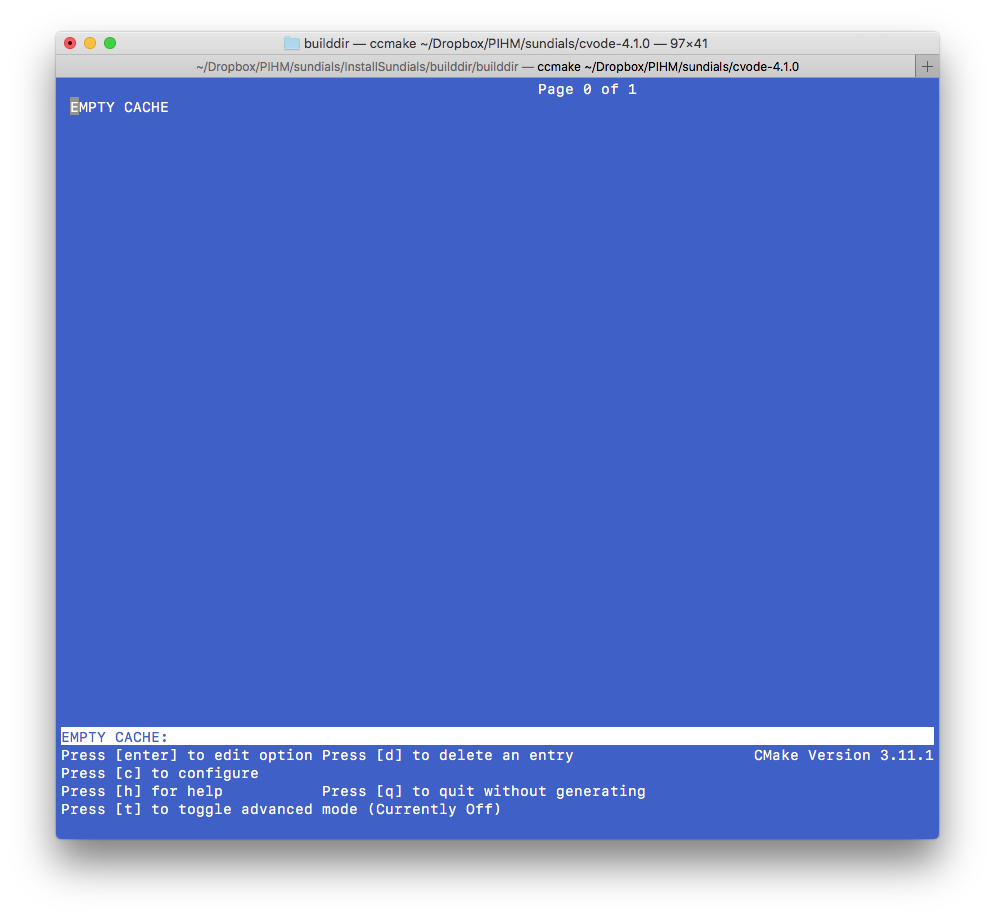
\includegraphics{Fig/ccmake/1.png} This is an empty configure. Press
  \texttt{c} to start the configuration.
\end{enumerate}

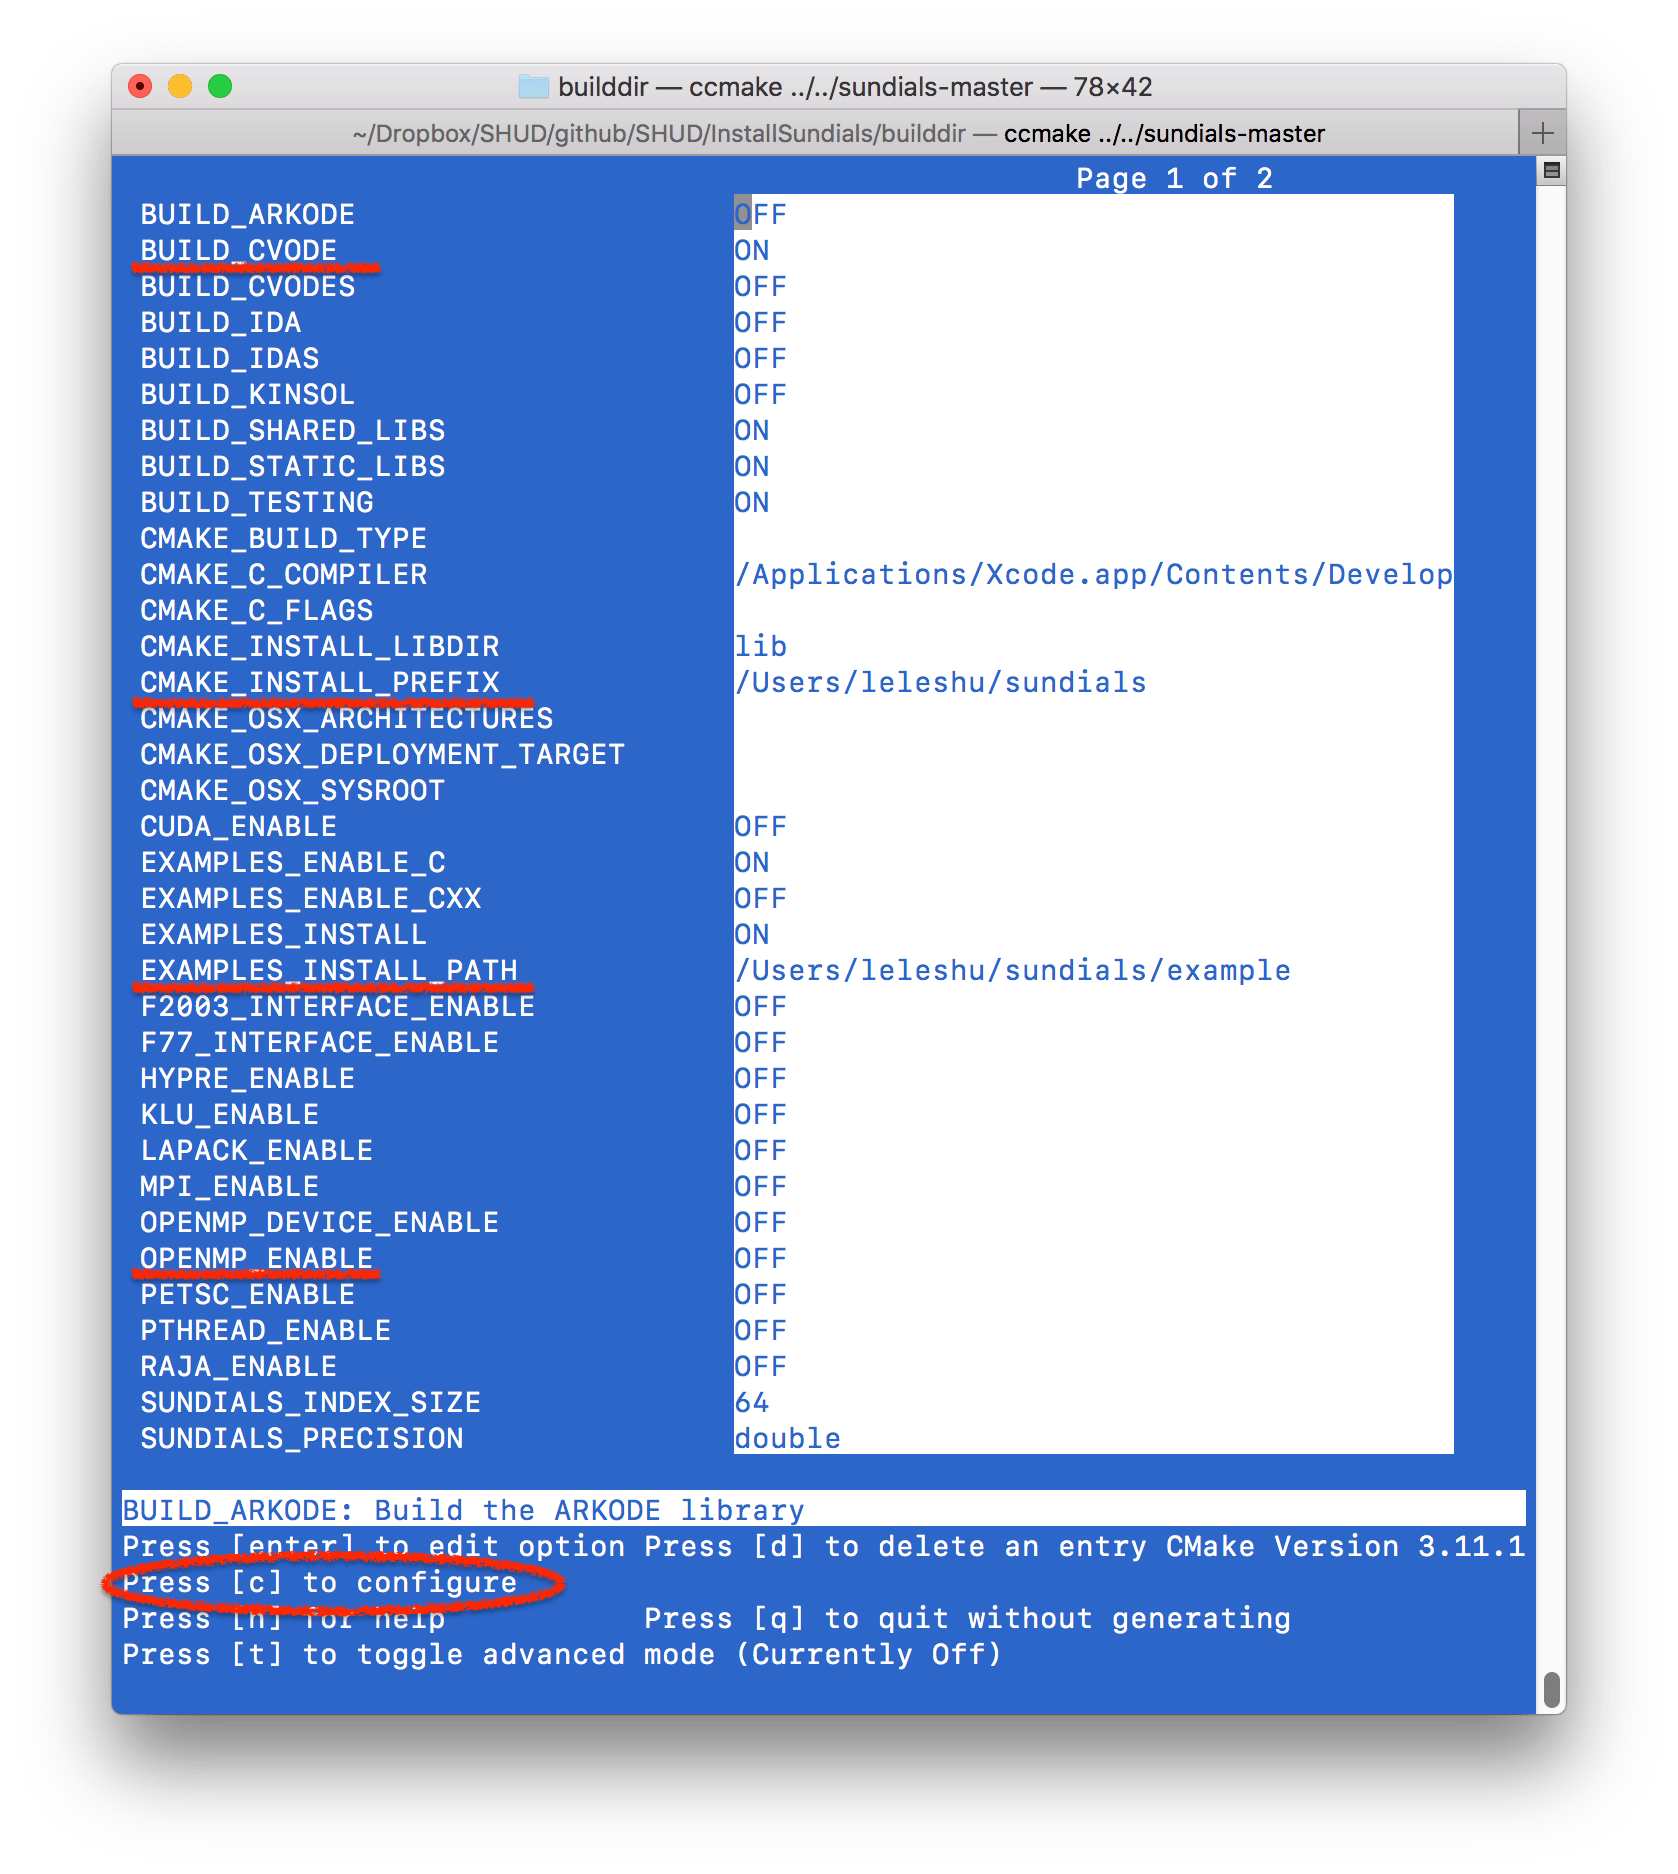
\includegraphics{Fig/ccmake/2.png} The default configuration. Make sure
the value for three lines:

\begin{verbatim}
BUILD_CVODE = ON
CMAKE_INSTALL_PREFIX = ~/sundials
EXAMPLES_INSTALL_PATH = ~/sundials/examples
\end{verbatim}

After the modification of values, press \texttt{c} to confirm
configuration.

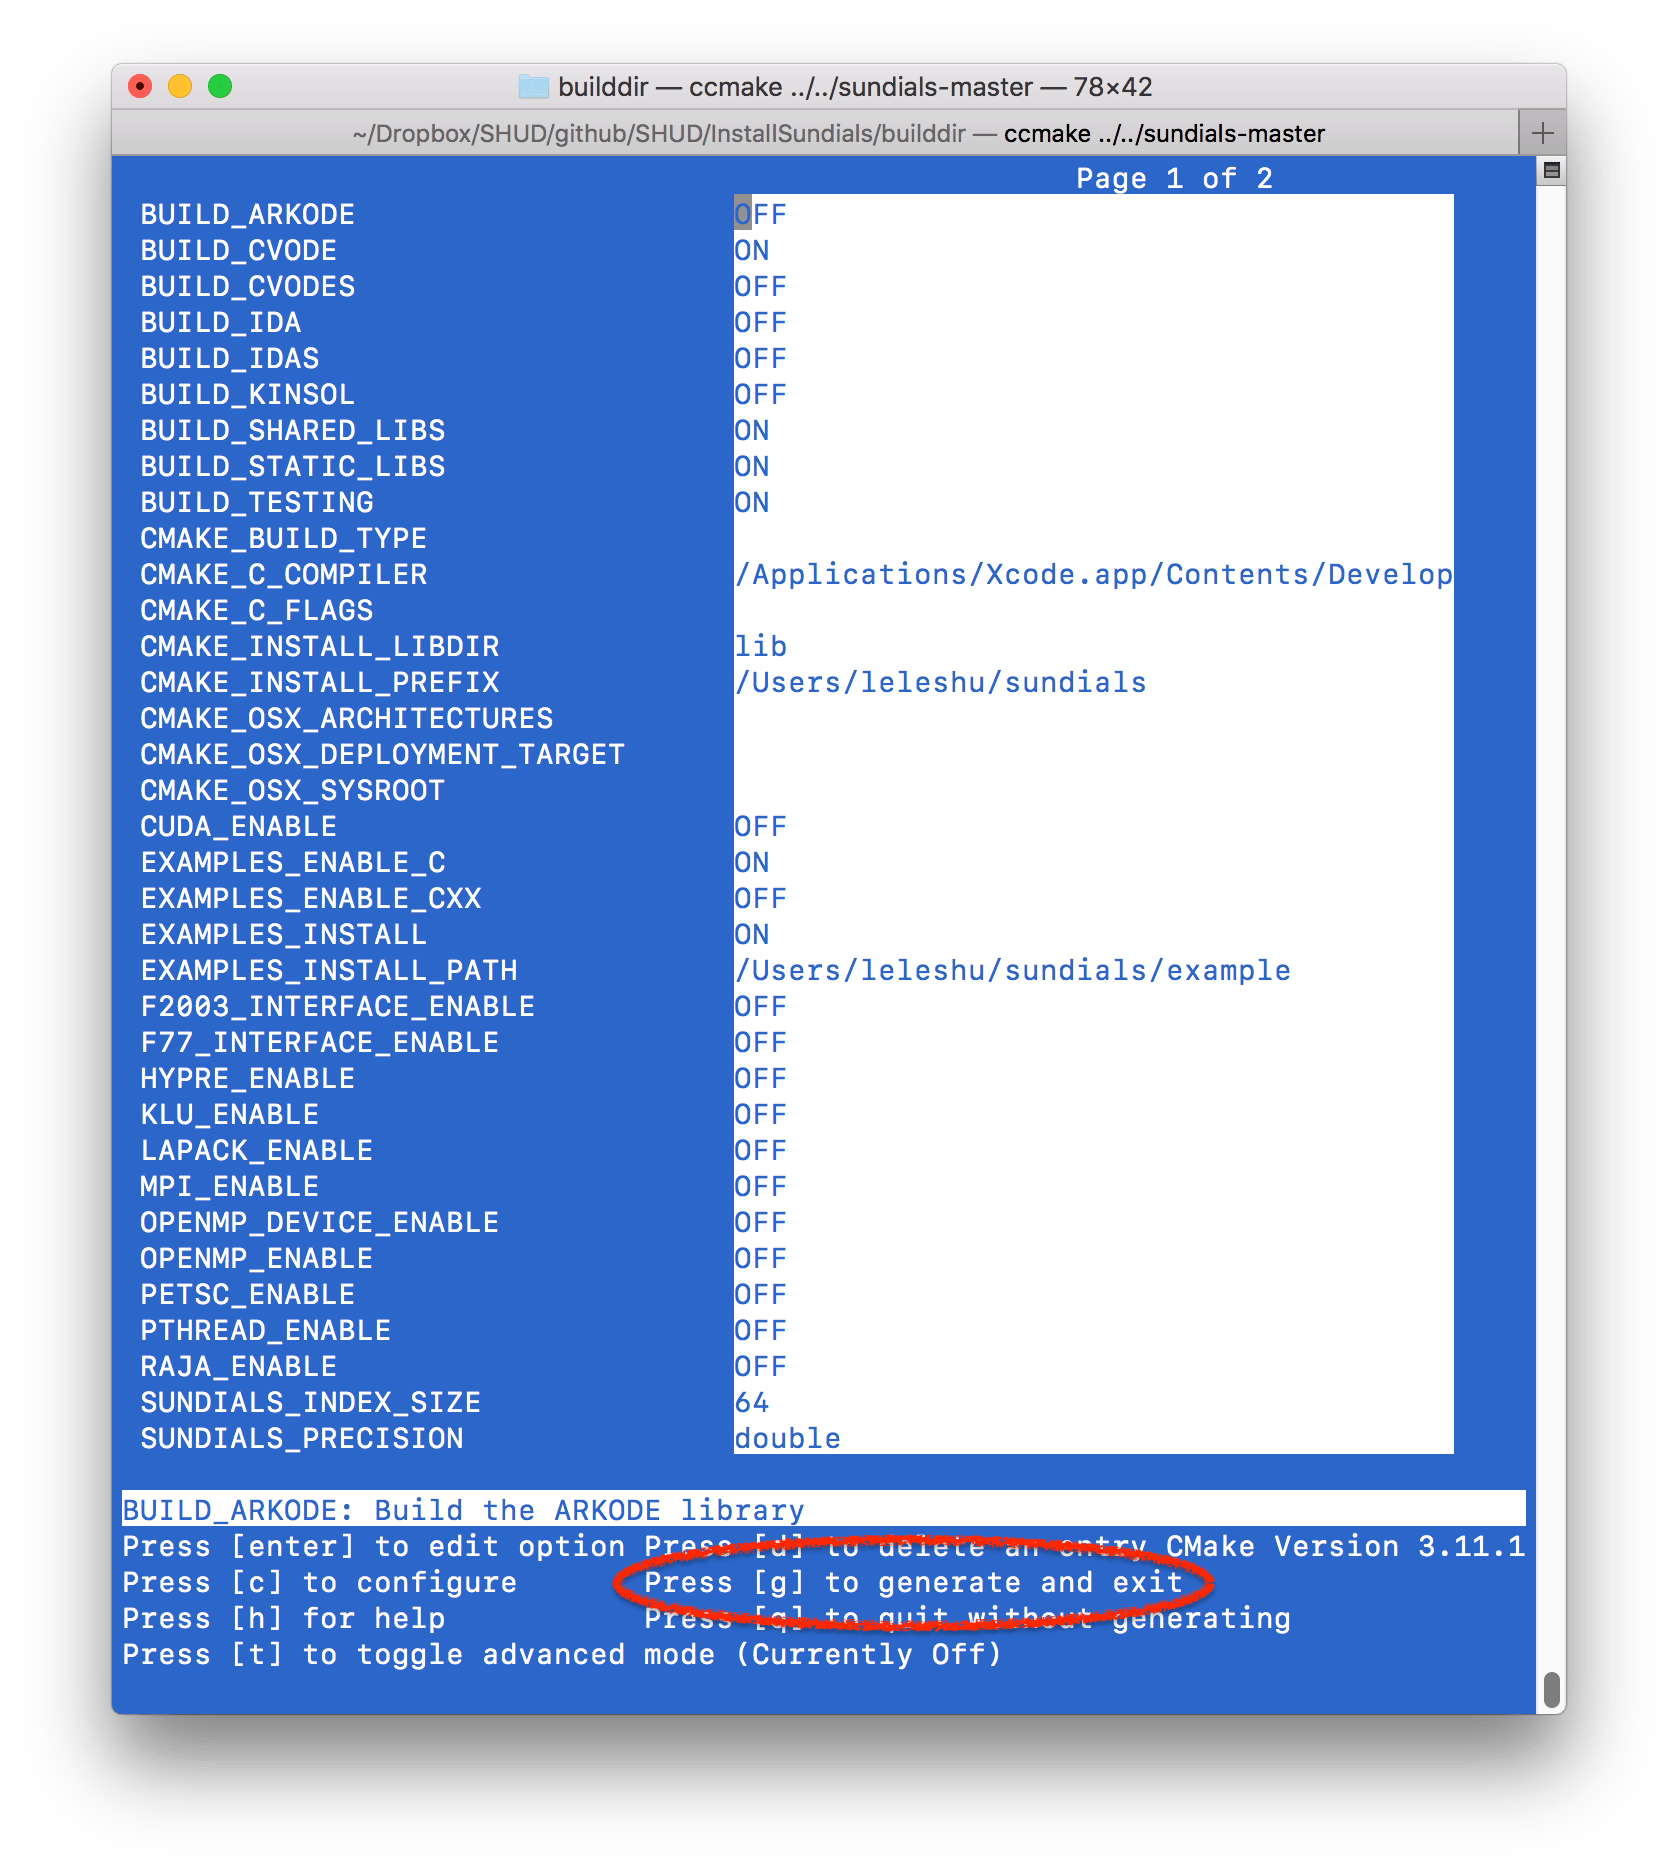
\includegraphics{Fig/ccmake/3.png} The ccmake configures the environment
automatically. When the configuration is ready, press \texttt{g} to
generate and exit.

\begin{enumerate}
\def\labelenumi{\arabic{enumi}.}
\item
  Then you run commands below:

\begin{verbatim}
make
make install 
\end{verbatim}
\end{enumerate}

\section{SHUD}\label{shud}

Configuration in \emph{Makefile}:

\begin{enumerate}
\def\labelenumi{\arabic{enumi}.}
\tightlist
\item
  Path of \emph{SUNDIALS\_DIR.} {[}\textbf{CRITICAL}{]}. If you install
  SUNDIALS into \emph{\textasciitilde{}/sundials}, you don't change this
  line..
\item
  Path of OpenMP if the parallel is preferred.
\item
  Path of SRC\_DIR, default is \texttt{SRC\_DIR\ =\ .}
\item
  Path of BUILT\_DIR, default is \texttt{BUILT\_DIR\ =\ .}
\end{enumerate}

After updating the SUNDIALS path in the \emph{Makefile}, user can
compile the SHUD with:

\begin{verbatim}
make clean
make shud
\end{verbatim}

There are more options to compile the SHUD code:

\begin{itemize}
\tightlist
\item
  \texttt{make\ all} - clean, then make both shud and shud\_omp
\item
  \texttt{make\ help} - help information
\item
  \texttt{make\ shud} - make SHUD executable
\item
  \texttt{make\ shud\_omp} - make shud\_omp with OpenMP support
\end{itemize}

\subsection{OpenMP}\label{openmp}

If parallel-computing is prefered, please install OpenMP. For mac:

\begin{verbatim}
brew install llvm clang
brew install libomp
compile flags for OpenMP: 
  -Xpreprocessor -fopenmp -lomp
Library/Include paths:
  -L/usr/local/opt/libomp/lib 
  -I/usr/local/opt/libomp/include
\end{verbatim}

\subsection{Run SHUD executables.}\label{run-shud-executables.}

After the successful installation and compile, you can run SHUD models
using

\begin{verbatim}
./shud <projectname>
\end{verbatim}

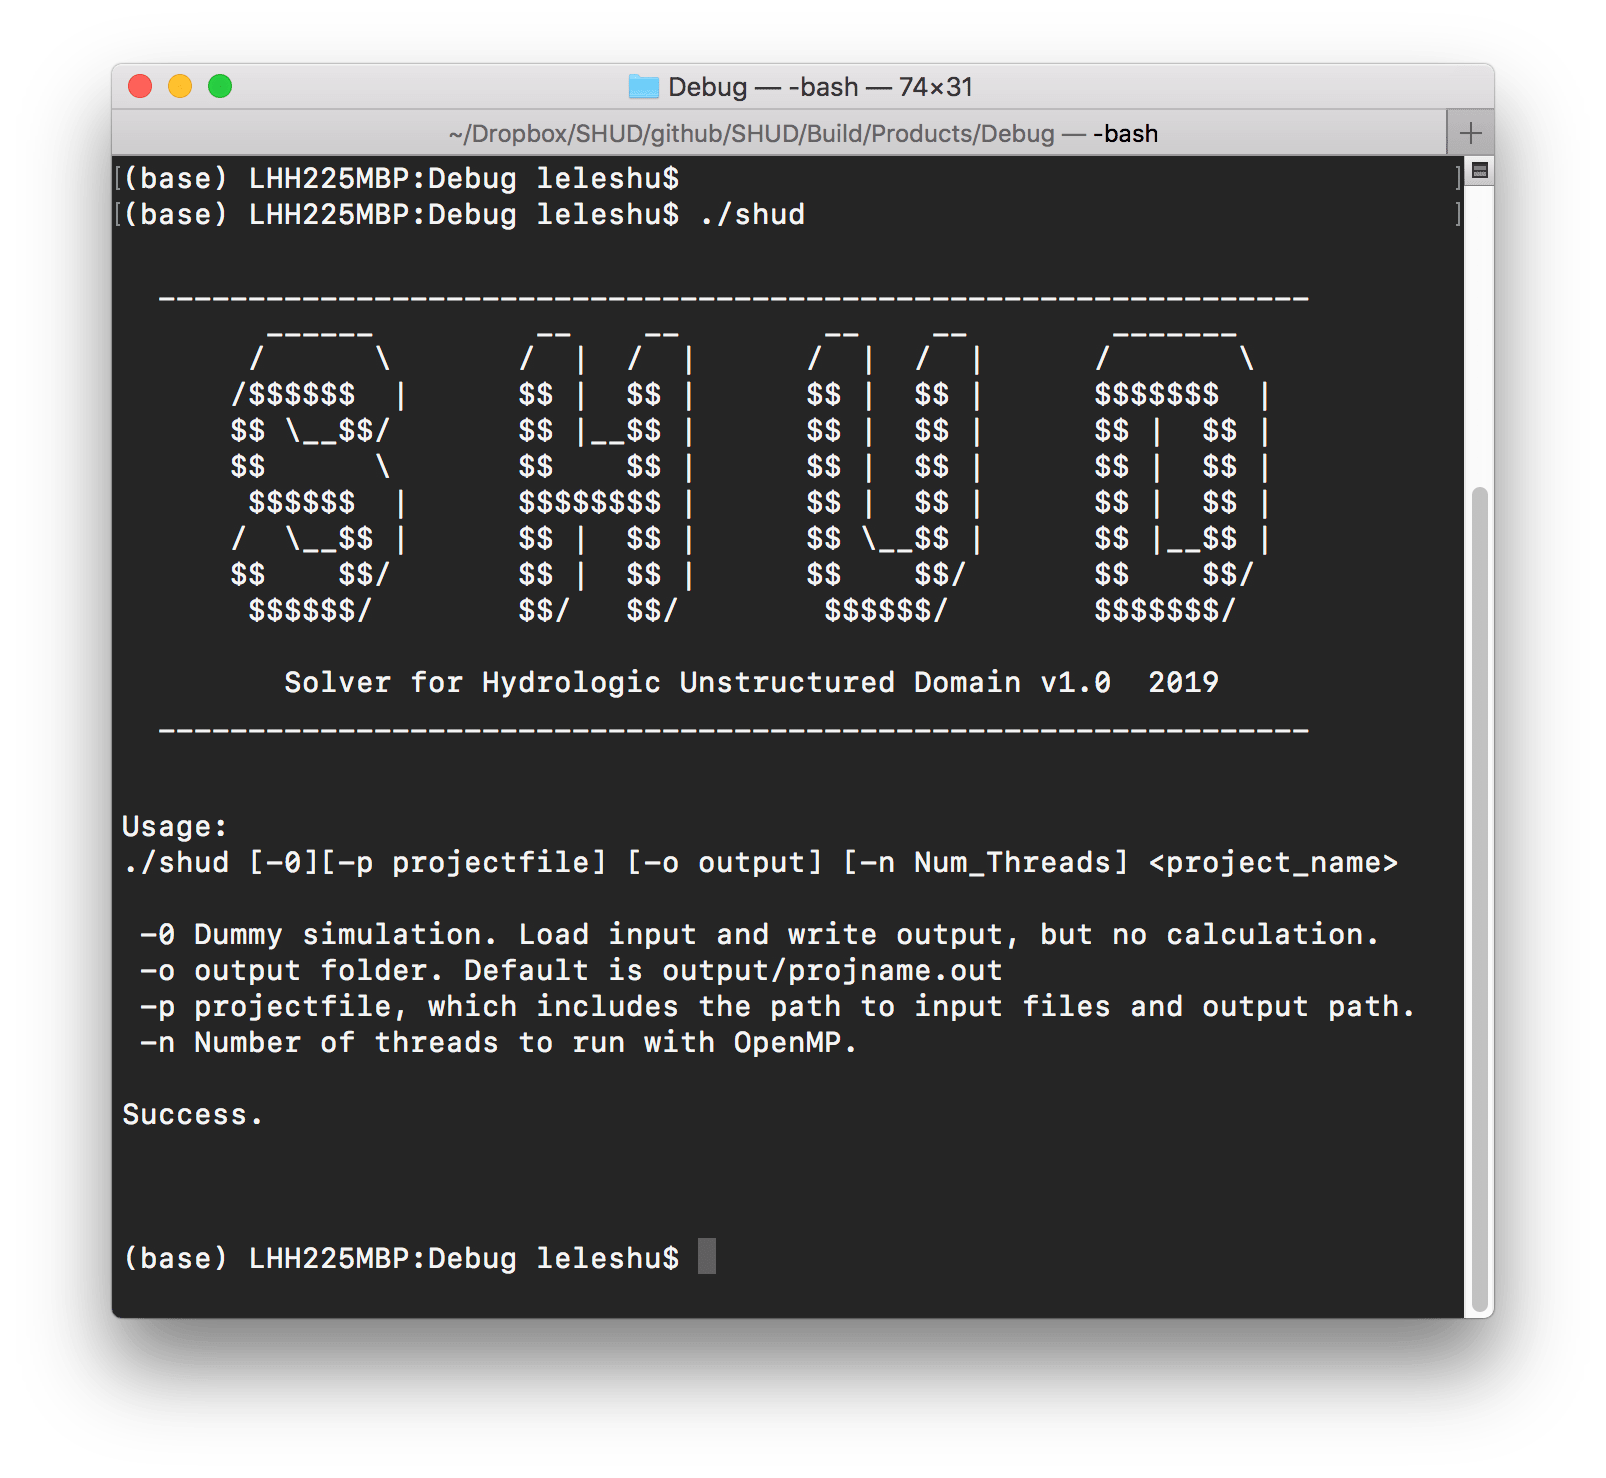
\includegraphics{Fig/CLI.png} Command line pattern is:

\begin{verbatim}
./shud [-0][-p projectfile] [-o output] [-n Num_Threads] <project_name>
\end{verbatim}

\begin{itemize}
\item
  \texttt{-0} Dummy simulation. Load input and write output, but no
  calculation.
\item
  \texttt{\textless{}project\ name\textgreater{}} is the name of the
  project.
\item
  \texttt{{[}-p\ projectfile{]}} Specify the project file, which
  includes the path to input files and output path.
\item
  \texttt{{[}-o\ output\_folder{]}} Output directory. Default is
  output/projname.out
\item
  \texttt{{[}-n\ Num\_Threads{]}} Number of threads to run with OpenMP,
  which works with \texttt{shud\_omp} only. Usage:
\end{itemize}

When the \texttt{shud} program starts to run, the screen should look
like this: 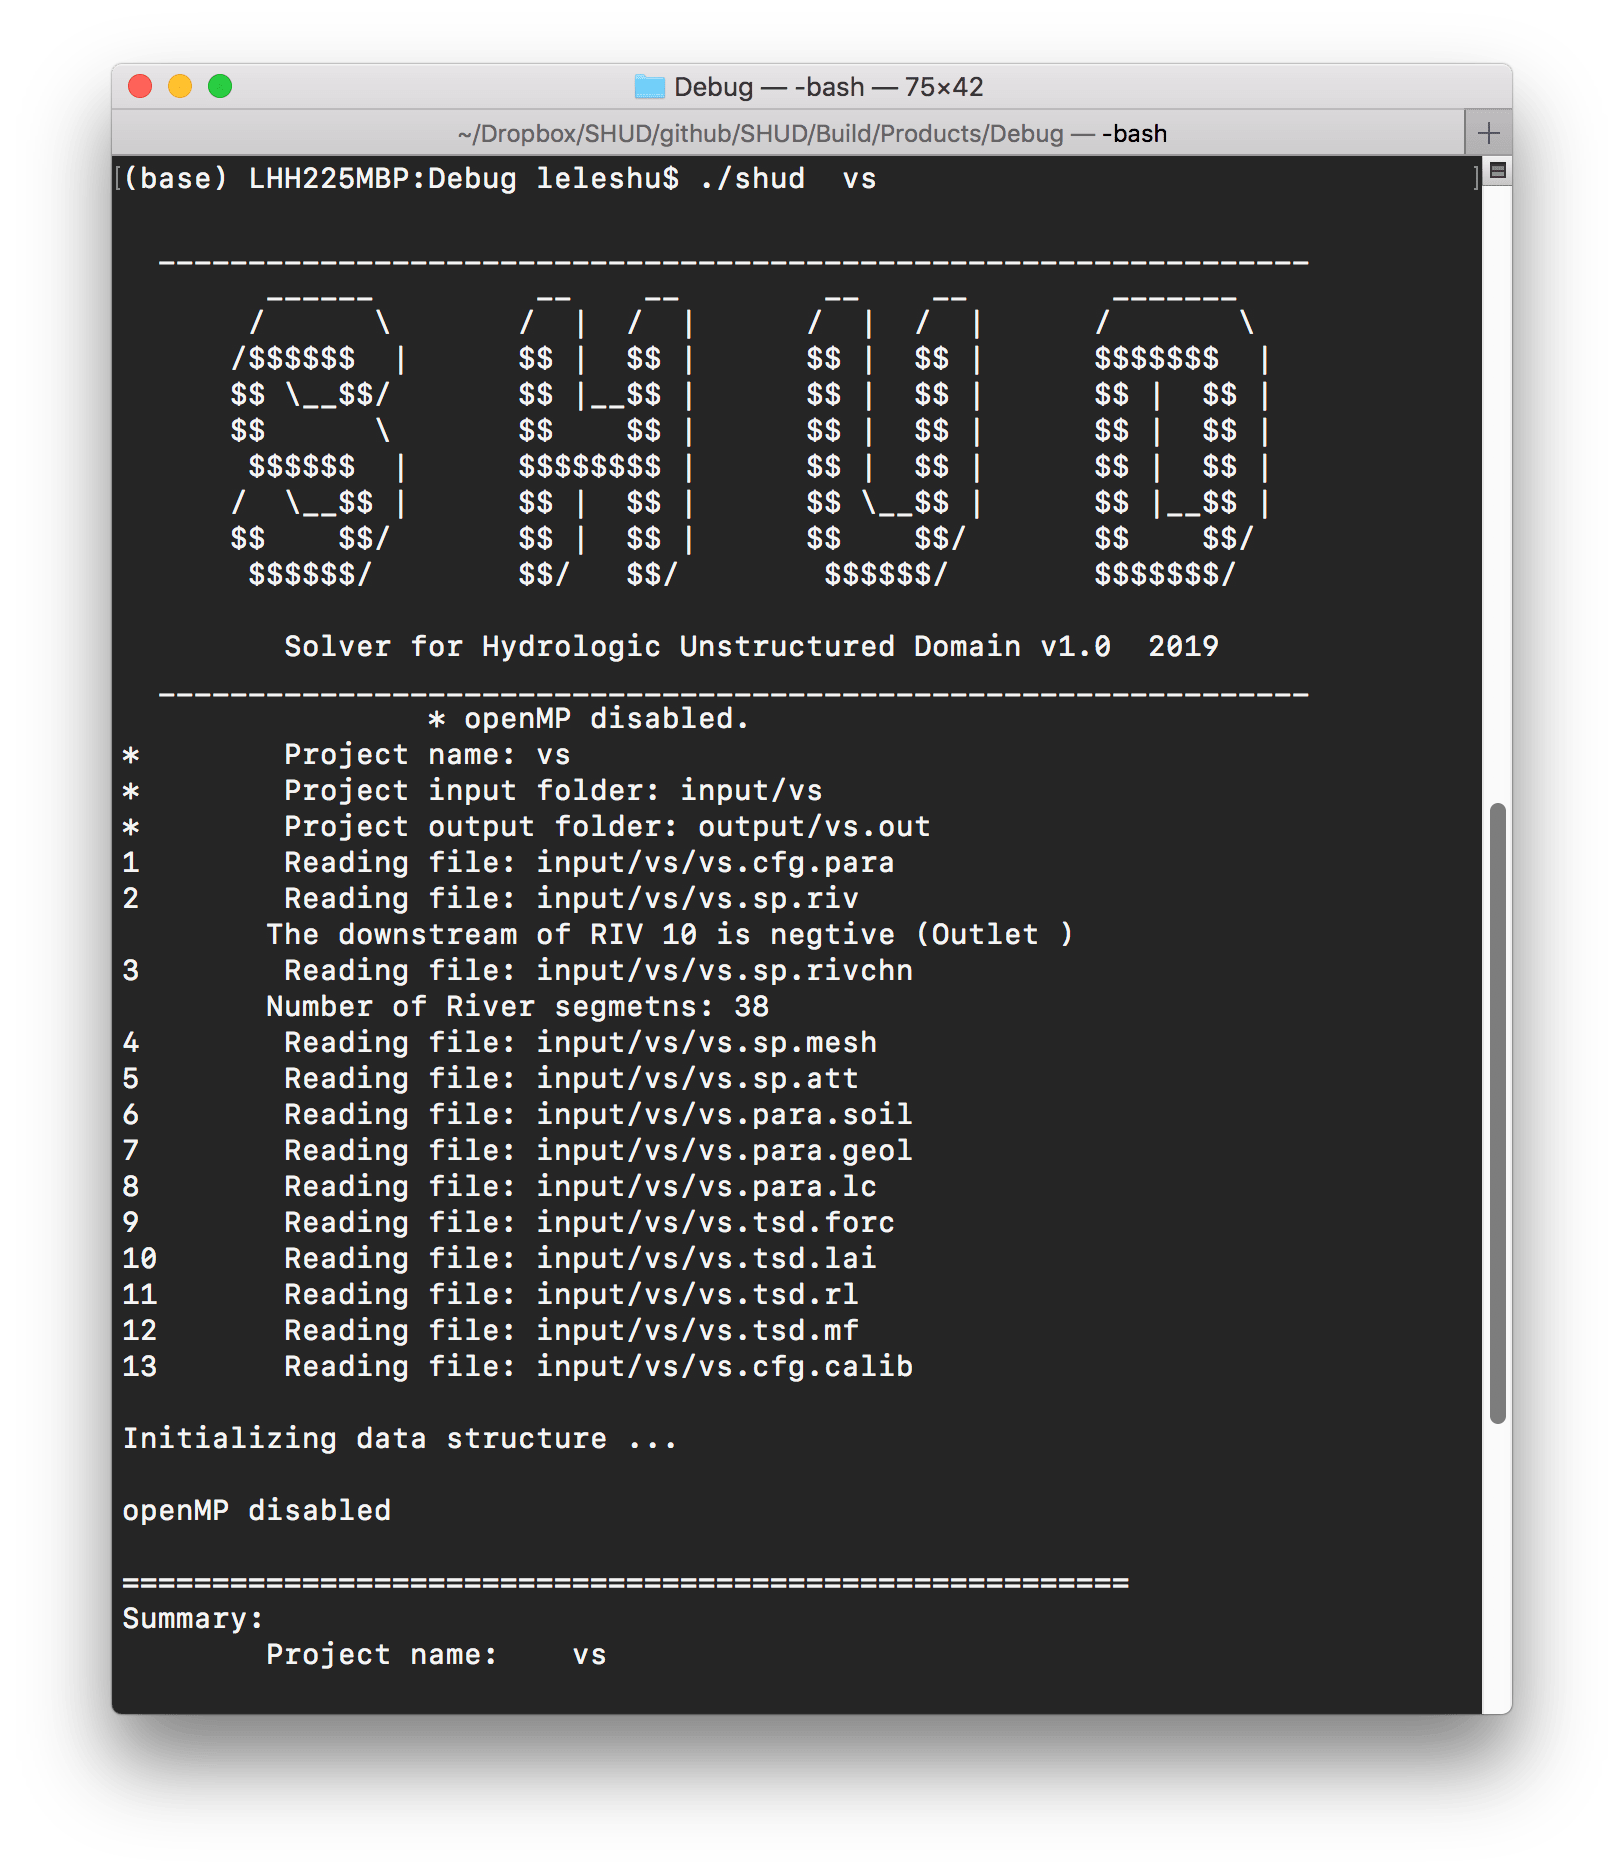
\includegraphics{Fig/CLI_vs.png}

\section{SHUDtoolbox}\label{shudtoolbox}

This SHUDtoolbox is an R package. What you need is to install the
package as a source code package. For example:

\begin{verbatim}
install_github('SHUD-System/SHUDtoolbox')
\end{verbatim}

The prerequisite packages for SHUDtoolbox are:

\begin{itemize}
\tightlist
\item
  Rcpp
\item
  reshape2
\item
  ggplot2
\item
  gridExtra
\item
  grid
\item
  fields
\item
  xts
\item
  hydroGOF
\item
  zoo
\item
  raster (\textgreater{}= 2.1.0)
\item
  sp
\item
  rgeos
\item
  RTriangle
\item
  rgdal (\textgreater{}= 1.1.0)
\item
  proj4
\item
  abind
\item
  utils
\item
  lubridate
\item
  geometry
\item
  methods
\item
  ncdf4
\item
  GGally
\item
  doParallel
\end{itemize}

One of the required packages, RTriangle, must be installed via GitHub
instead of CRAN, using command:

\begin{verbatim}
install_github('shulele/RTriangle/pkg') 
\end{verbatim}

\chapter{Input files}\label{input-files}

List of input files:

\begin{longtable}[]{@{}ccccc@{}}
\toprule
File & Category & Comments & Header & \# of column\tabularnewline
\midrule
\endhead
.mesh & sp & Domain cell (triangular mesh) & Yes &\tabularnewline
.att & sp & Attribute table of triangular cells & Yes &\tabularnewline
.riv & sp & Rivers & Yes &\tabularnewline
.rivseg & sp & Topologic relation b/w River and cell & Yes
&\tabularnewline
.calib & cfg & Calibration on physical parameters & Yes &\tabularnewline
.para & cfg & Parameters of the model configurature & Yes
&\tabularnewline
.ic & cfg & Intial conditions & Yes &\tabularnewline
.geol & para & Physical parameters for Geology layers & Yes
&\tabularnewline
.soil & para & Physical parameters for Soil layers & Yes
&\tabularnewline
.lc & para & Physical parameters for Land cover layers & Yes
&\tabularnewline
.forc & tsd & List of files to the Time-series forcing data & Yes
&\tabularnewline
.csv & tsd & Time-series forcing data & Yes &\tabularnewline
.lai & tsd & Time-series LAI data & Yes &\tabularnewline
.obs & tsd & Time-series observational data for calibration purpose only
& Yes &\tabularnewline
.mf & tsd & Time-series Melt Factor data & Yes &\tabularnewline
.rl & tsd & Time-series Roughness Length data & Yes &\tabularnewline
gis/domain & Shapefile & Shapefile of .mesh file & x & x\tabularnewline
gis/river & Shapefile & Shapefile of .riv file & x & x\tabularnewline
gis/seg & Shapefile & Shapefile of .rivchn file & x & x\tabularnewline
\bottomrule
\end{longtable}

\begin{figure}
\centering
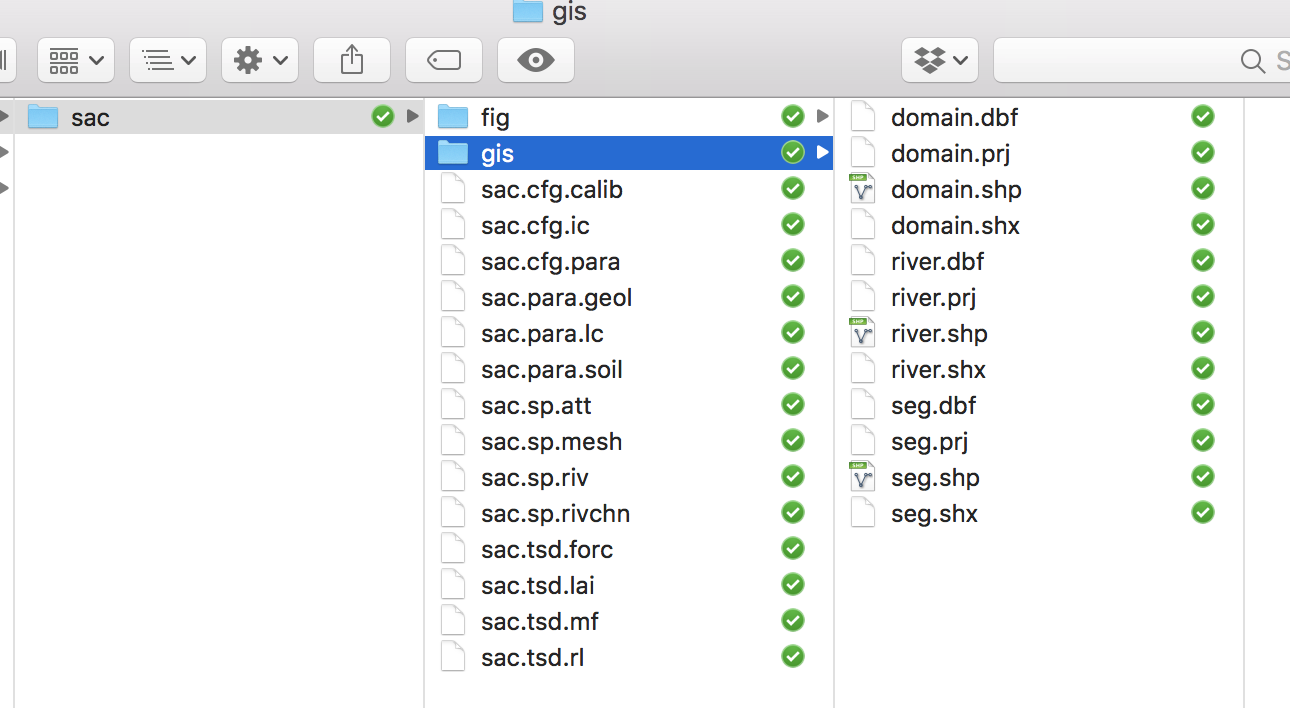
\includegraphics{Fig/IO/Inputfiles.png}
\caption{The screenshot of input files for SHUD}
\end{figure}

The files in folder \emph{gis} and \emph{fig} are not involved in SHUD
modeling, but they are very useful for your data pre- and
post-processing.

\section{Spatial data}\label{spatial-data}

\subsection{.sp.mesh file}\label{sp.mesh-file}

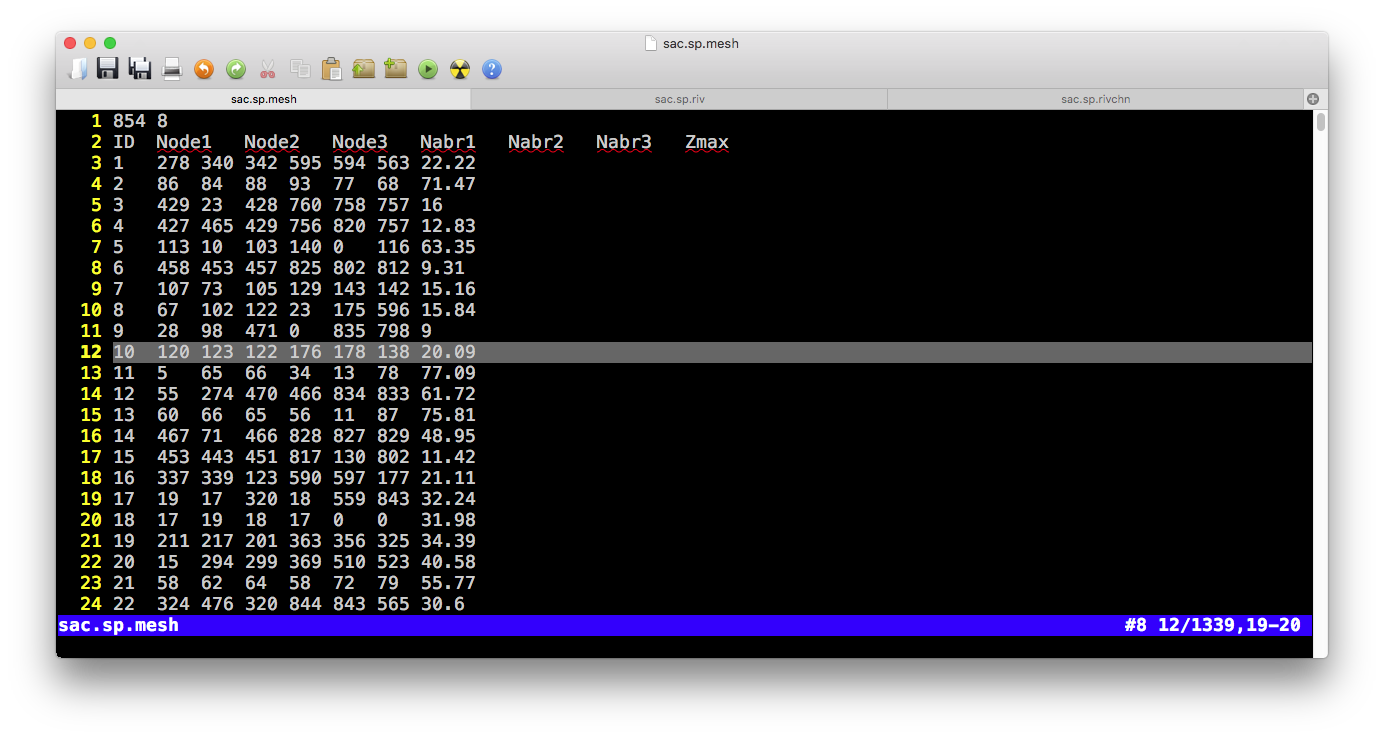
\includegraphics{Fig/IO/sp.mesh1.png}
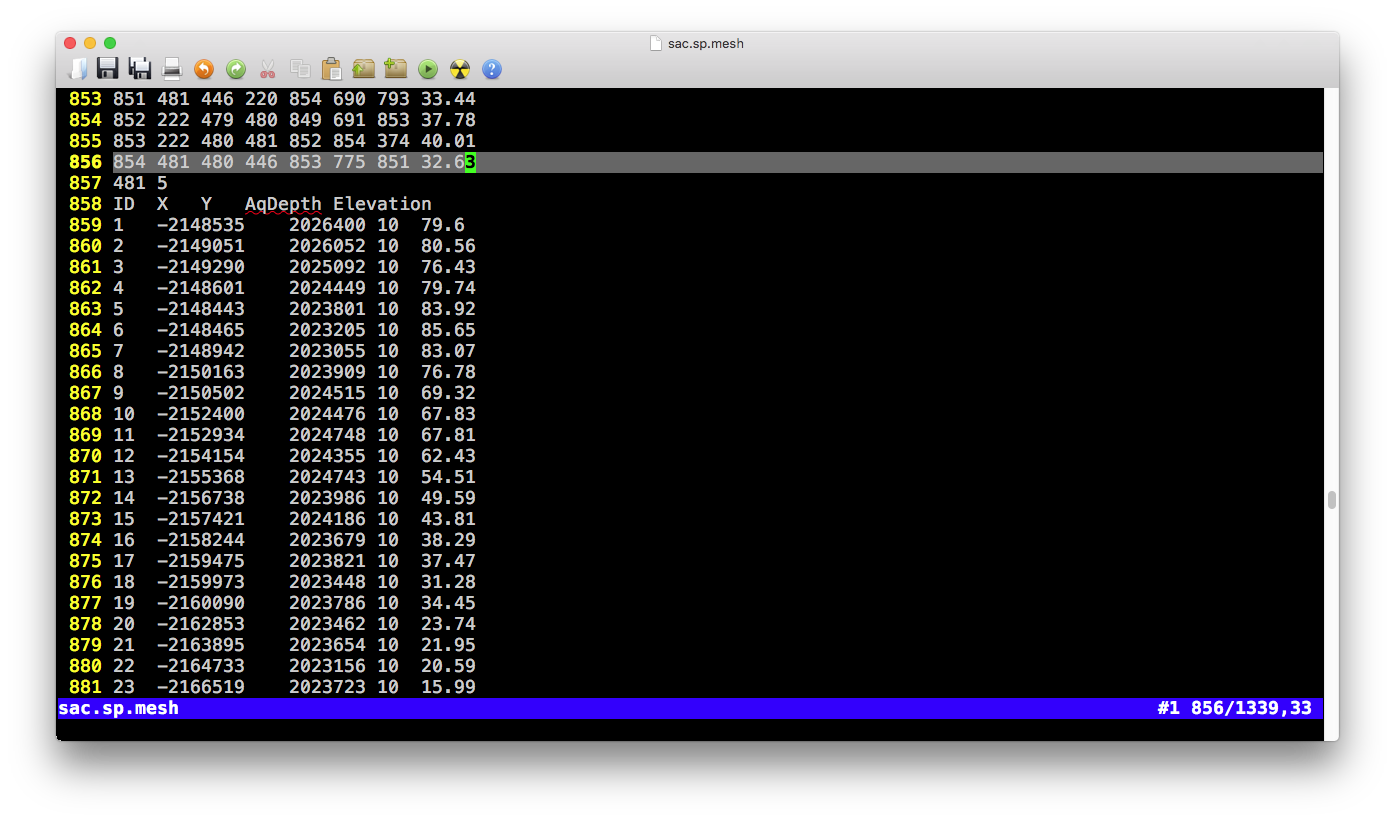
\includegraphics{Fig/IO/sp.mesh2.png} There are two tables in the .mesh
file, the one is a table of cells and the other is a table of nodes of
cells.

\begin{itemize}
\item
  \textbf{Block 1 (cell information)}
\item
  Pre-table
\end{itemize}

\begin{longtable}[]{@{}cc@{}}
\toprule
Value1 & Value2\tabularnewline
\midrule
\endhead
Number of rows ( \(N_{cell}\)) & Number of columns
(\(8\))\tabularnewline
\bottomrule
\end{longtable}

\begin{itemize}
\tightlist
\item
  Table
\end{itemize}

\begin{longtable}[]{@{}ccccc@{}}
\toprule
Colname & Meaning & Range & Unit & Comments\tabularnewline
\midrule
\endhead
ID & Index of cell \(i\) & 1 \textasciitilde{} \(N_{cell}\) & -
&\tabularnewline
Node1 & Node 1 of cell \(i\) & 1 \textasciitilde{} \(N_{node}\) & -
&\tabularnewline
Node2 & Node 2 of cell \(i\) & 1 \textasciitilde{} \(N_{node}\) & -
&\tabularnewline
Node3 & Node 3 of cell \(i\) & 1 \textasciitilde{} \(N_{node}\) & -
&\tabularnewline
Nabr1 & Index of Neighbor 1 of cell \(i\) & 1 \textasciitilde{}
\(N_{cell}\) & - &\tabularnewline
Nabr2 & Index of Neighbor 2 of cell \(i\) & 1 \textasciitilde{}
\(N_{cell}\) & - &\tabularnewline
Nabr3 & Index of Neighbor 3 of cell \(i\) & 1 \textasciitilde{}
\(N_{cell}\) & - &\tabularnewline
Zmax & Surface elevation of cell \(i\) & -9999 \textasciitilde{} +inf &
\(m\) &\tabularnewline
\bottomrule
\end{longtable}

\begin{itemize}
\item
  \textbf{Block 2 (node information)}
\item
  Pre-table:
\end{itemize}

\begin{longtable}[]{@{}cc@{}}
\toprule
Value1 & Value2\tabularnewline
\midrule
\endhead
Number of rows ( \(N_{node}\)) & Number of columns
(\(5\))\tabularnewline
\bottomrule
\end{longtable}

\begin{itemize}
\tightlist
\item
  Table
\end{itemize}

\begin{longtable}[]{@{}ccccc@{}}
\toprule
Colname & Meaning & Range & Unit & Comments\tabularnewline
\midrule
\endhead
ID & Index of node \(i\) & 1 \textasciitilde{} \(N_{cell}\) & -
&\tabularnewline
X & X coordinate of node \(i\) & 1 \textasciitilde{} \(N_{node}\) & -
&\tabularnewline
Y & Y coordinate of node \(i\) & 1 \textasciitilde{} \(N_{node}\) & -
&\tabularnewline
AqDepth & Thickness of aquifer \(i\) & 0 \textasciitilde{} +inf & \(m\)
&\tabularnewline
Elevation & Surface elevation of node \(i\) & -9999 \textasciitilde{}
+inf & \(m\) &\tabularnewline
\bottomrule
\end{longtable}

\subsection{.sp.att file}\label{sp.att-file}

\begin{figure}
\centering
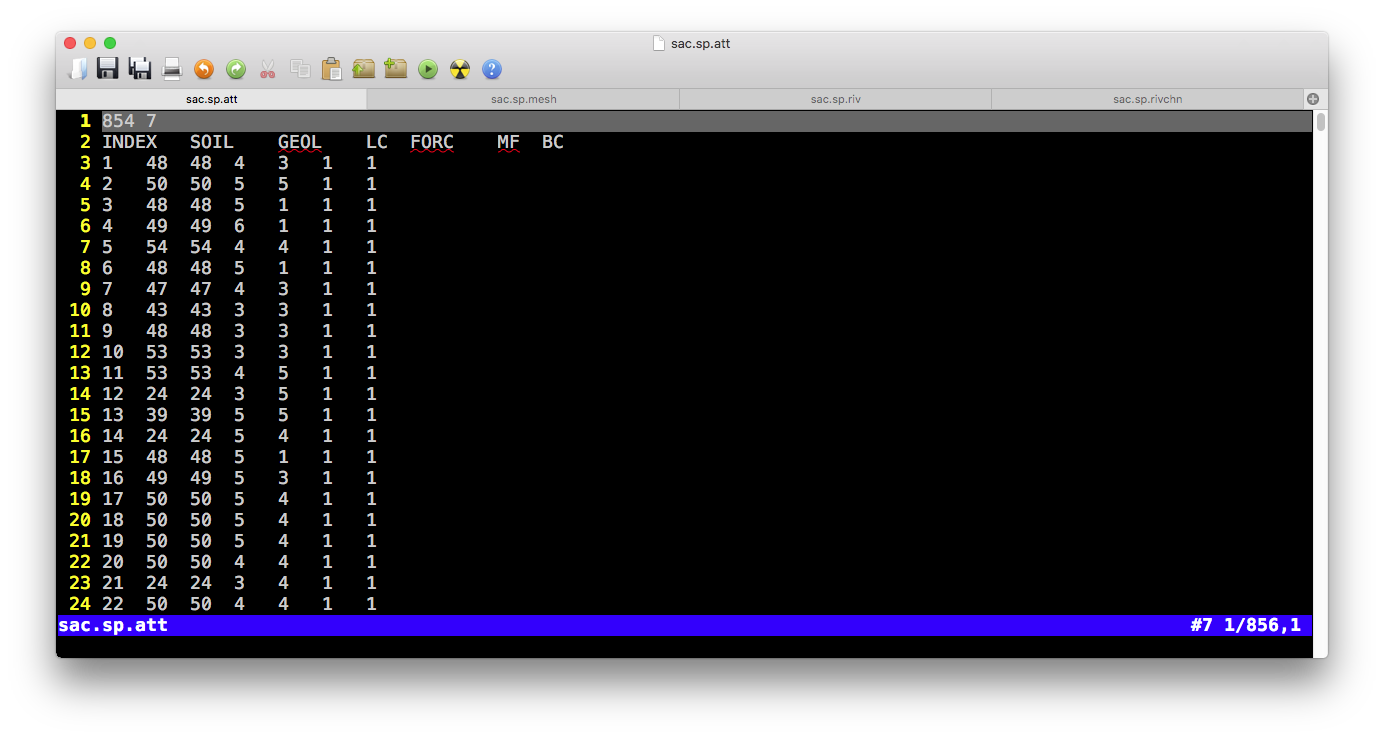
\includegraphics{Fig/IO/sp.att.png}
\caption{Example of .sp.att file}
\end{figure}

\begin{itemize}
\tightlist
\item
  Pre-table
\end{itemize}

\begin{longtable}[]{@{}cc@{}}
\toprule
Value1 & Value2\tabularnewline
\midrule
\endhead
Number of rows ( \(N_{cell}\)) & Number of columns
(\(7\))\tabularnewline
\bottomrule
\end{longtable}

\begin{itemize}
\tightlist
\item
  Table
\end{itemize}

\begin{longtable}[]{@{}ccccc@{}}
\toprule
Colname & Meaning & Range & Unit & Comments\tabularnewline
\midrule
\endhead
ID & Index of cell \(i\) & 1 \textasciitilde{} \(N_{cell}\) & -
&\tabularnewline
SOIL & Index of soil type & 1 \textasciitilde{} \(N_{soil}\) & -
&\tabularnewline
GEOL & Index of geology type & 1 \textasciitilde{} \(N_{geol}\) & -
&\tabularnewline
LC & Index of land cover type & 1 \textasciitilde{} \(N_{lc}\) & - &
\(N_{lc}\) = \(N_{lai}\)\tabularnewline
FORC & Index of forcing site & 1 \textasciitilde{} \(N_{forc}\) & -
&\tabularnewline
MF & Index of melt factor & 1 \textasciitilde{} \(N_{mf}\) & -
&\tabularnewline
BC & Index of boundary condition & 1 \textasciitilde{} \(N_{bc}\) & -
&\tabularnewline
SS & Index of Source/Sink condition & 1 \textasciitilde{} \(N_{bc}\) & -
&\tabularnewline
\bottomrule
\end{longtable}

\subsection{.sp.riv file}\label{sp.riv-file}

\begin{figure}
\centering
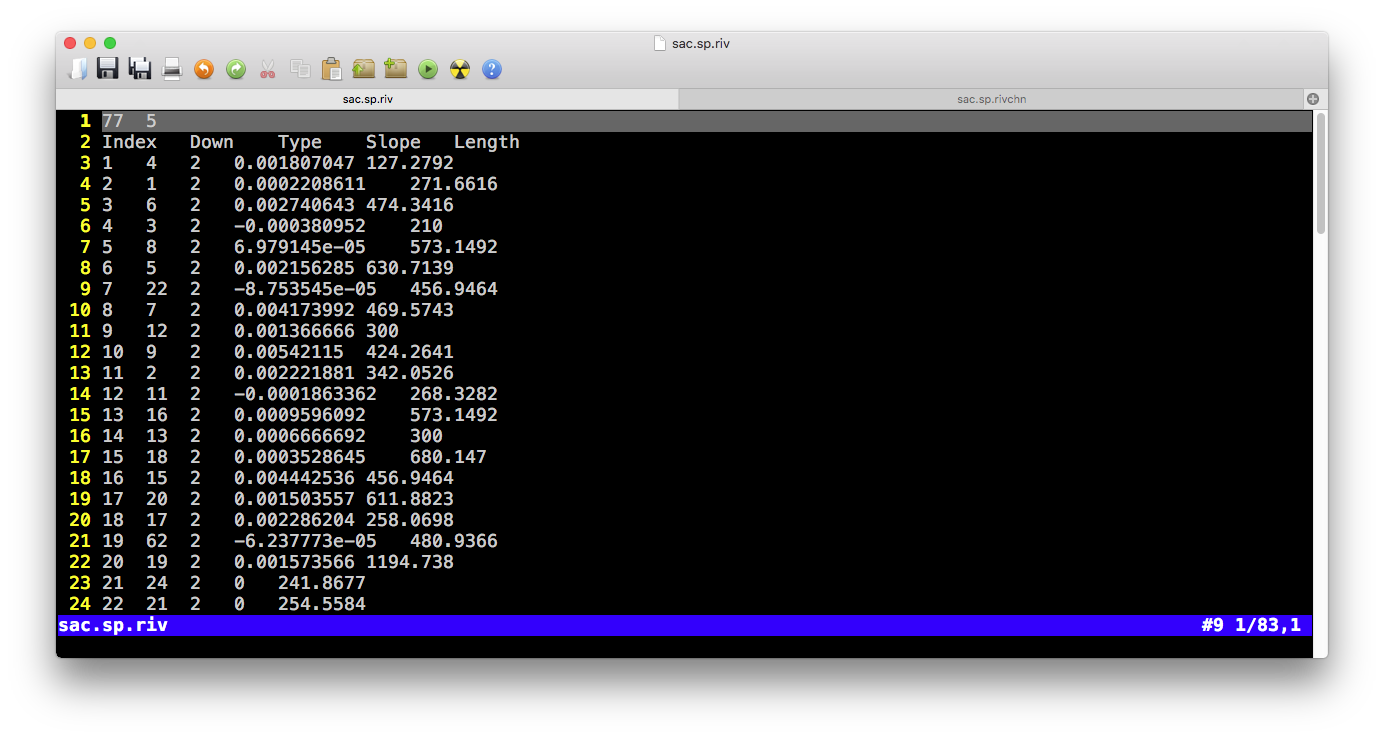
\includegraphics{Fig/IO/sp.riv.png}
\caption{Example of .sp.riv file}
\end{figure}

\begin{itemize}
\tightlist
\item
  Pre-table
\end{itemize}

\begin{longtable}[]{@{}cc@{}}
\toprule
Value1 & Value2\tabularnewline
\midrule
\endhead
Number of rows ( \(N_{riv}\)) & Number of columns (\(5\))\tabularnewline
\bottomrule
\end{longtable}

\begin{itemize}
\tightlist
\item
  Table
\end{itemize}

\begin{longtable}[]{@{}ccccc@{}}
\toprule
\begin{minipage}[b]{0.11\columnwidth}\centering\strut
Colname\strut
\end{minipage} & \begin{minipage}[b]{0.25\columnwidth}\centering\strut
Meaning\strut
\end{minipage} & \begin{minipage}[b]{0.11\columnwidth}\centering\strut
Range\strut
\end{minipage} & \begin{minipage}[b]{0.11\columnwidth}\centering\strut
Unit\strut
\end{minipage} & \begin{minipage}[b]{0.29\columnwidth}\centering\strut
Comments\strut
\end{minipage}\tabularnewline
\midrule
\endhead
\begin{minipage}[t]{0.11\columnwidth}\centering\strut
ID\strut
\end{minipage} & \begin{minipage}[t]{0.25\columnwidth}\centering\strut
Index of river \(i\)\strut
\end{minipage} & \begin{minipage}[t]{0.11\columnwidth}\centering\strut
1 \textasciitilde{} \(N_{river}\)\strut
\end{minipage} & \begin{minipage}[t]{0.11\columnwidth}\centering\strut
-\strut
\end{minipage} & \begin{minipage}[t]{0.29\columnwidth}\centering\strut
\strut
\end{minipage}\tabularnewline
\begin{minipage}[t]{0.11\columnwidth}\centering\strut
DOWN\strut
\end{minipage} & \begin{minipage}[t]{0.25\columnwidth}\centering\strut
Index of downstream river\strut
\end{minipage} & \begin{minipage}[t]{0.11\columnwidth}\centering\strut
1 \textasciitilde{} \(N_{river}\)\strut
\end{minipage} & \begin{minipage}[t]{0.11\columnwidth}\centering\strut
-\strut
\end{minipage} & \begin{minipage}[t]{0.29\columnwidth}\centering\strut
Negative vlaue indicates outlet\strut
\end{minipage}\tabularnewline
\begin{minipage}[t]{0.11\columnwidth}\centering\strut
Type\strut
\end{minipage} & \begin{minipage}[t]{0.25\columnwidth}\centering\strut
Index of river parameters\strut
\end{minipage} & \begin{minipage}[t]{0.11\columnwidth}\centering\strut
1 \textasciitilde{} \(N_{rivertype}\)\strut
\end{minipage} & \begin{minipage}[t]{0.11\columnwidth}\centering\strut
-\strut
\end{minipage} & \begin{minipage}[t]{0.29\columnwidth}\centering\strut
\strut
\end{minipage}\tabularnewline
\begin{minipage}[t]{0.11\columnwidth}\centering\strut
Slope\strut
\end{minipage} & \begin{minipage}[t]{0.25\columnwidth}\centering\strut
Slope of river bed\strut
\end{minipage} & \begin{minipage}[t]{0.11\columnwidth}\centering\strut
-10 \textasciitilde{} 10\strut
\end{minipage} & \begin{minipage}[t]{0.11\columnwidth}\centering\strut
\(m/m\)\strut
\end{minipage} & \begin{minipage}[t]{0.29\columnwidth}\centering\strut
Height/Length\strut
\end{minipage}\tabularnewline
\begin{minipage}[t]{0.11\columnwidth}\centering\strut
Length\strut
\end{minipage} & \begin{minipage}[t]{0.25\columnwidth}\centering\strut
Length of the river \(i\)\strut
\end{minipage} & \begin{minipage}[t]{0.11\columnwidth}\centering\strut
0 \textasciitilde{} inf\strut
\end{minipage} & \begin{minipage}[t]{0.11\columnwidth}\centering\strut
\(m\)\strut
\end{minipage} & \begin{minipage}[t]{0.29\columnwidth}\centering\strut
\strut
\end{minipage}\tabularnewline
\bottomrule
\end{longtable}

\subsection{.sp.rivseg file}\label{sp.rivseg-file}

\begin{figure}
\centering
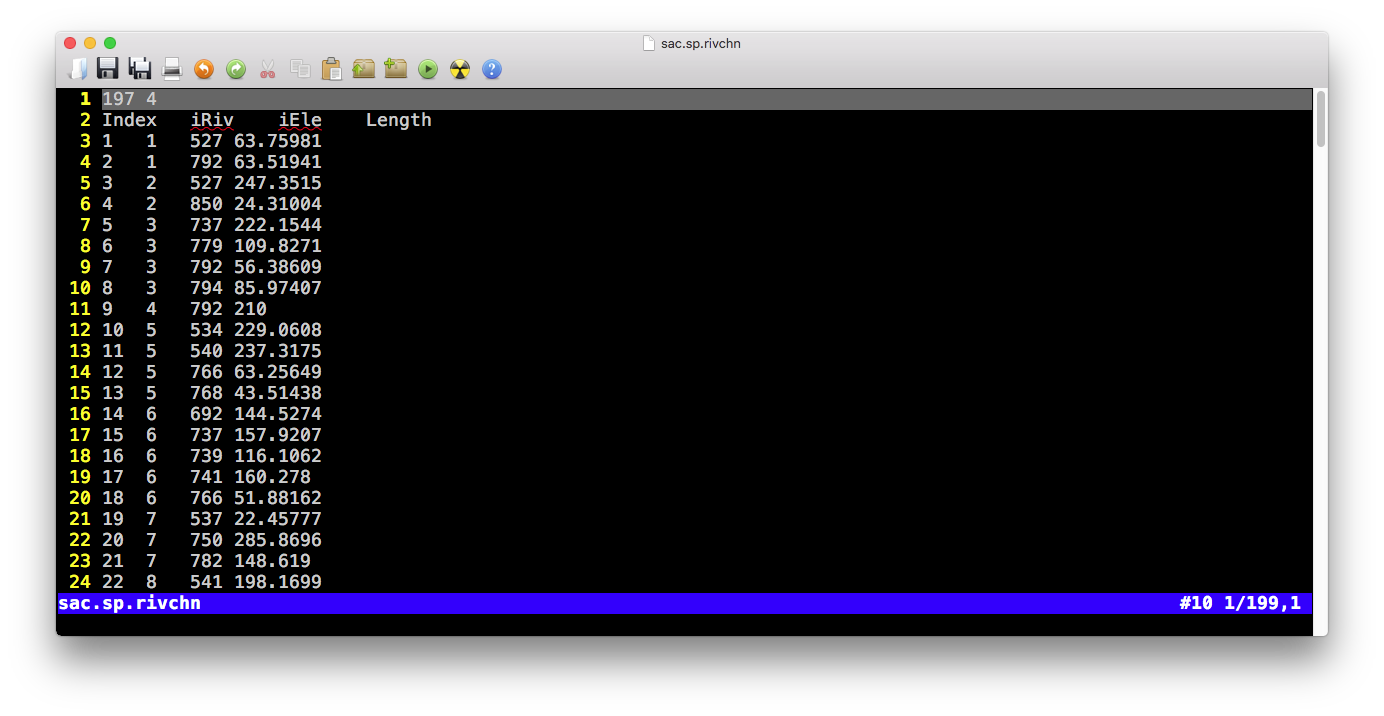
\includegraphics{Fig/IO/sp.rivchn.png}
\caption{Example of .sp.rivseg file}
\end{figure}

\begin{itemize}
\tightlist
\item
  Pre-table
\end{itemize}

\begin{longtable}[]{@{}cc@{}}
\toprule
Value1 & Value2\tabularnewline
\midrule
\endhead
Number of rows ( \(N_{segment}\)) & Number of columns
(\(4\))\tabularnewline
\bottomrule
\end{longtable}

\begin{itemize}
\tightlist
\item
  Table
\end{itemize}

\begin{longtable}[]{@{}ccccc@{}}
\toprule
Colname & Meaning & Range & Unit & Comments\tabularnewline
\midrule
\endhead
ID & Index of segments \(i\) & 1 \textasciitilde{} \(N_{segment}\) & -
&\tabularnewline
iRiv & Index of river & 1 \textasciitilde{} \(N_{river}\) & -
&\tabularnewline
iEle & Index of cell & 1 \textasciitilde{} \(N_{cell}\) & -
&\tabularnewline
Length & Length of the segments \(i\) & 0 \textasciitilde{} inf & \(m\)
&\tabularnewline
\bottomrule
\end{longtable}

\section{Model configuration files}\label{model-configuration-files}

\subsection{.cfg.para file}\label{cfg.para-file}

\begin{figure}
\centering
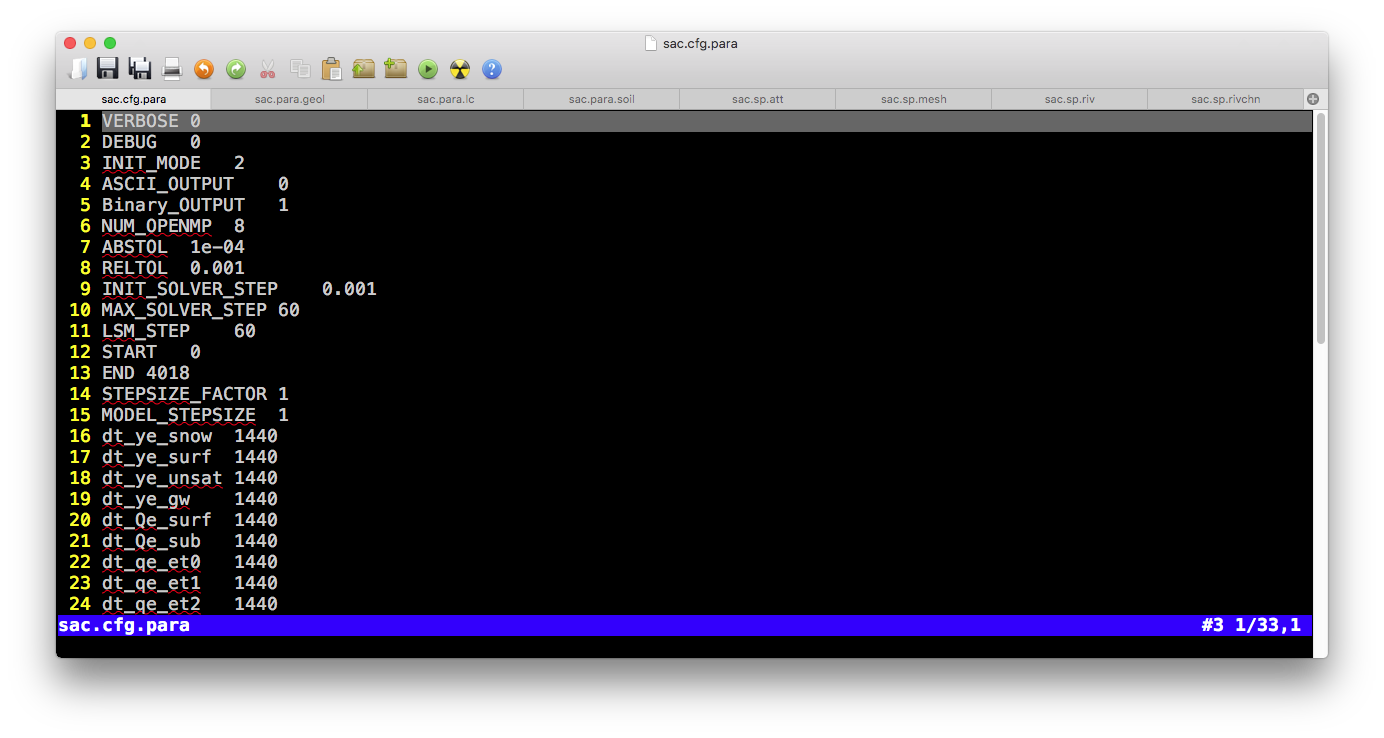
\includegraphics{Fig/IO/cfg.para.png}
\caption{Example of .cfg.para file}
\end{figure}

\begin{itemize}
\tightlist
\item
  Table
\end{itemize}

\begin{longtable}[]{@{}ccccc@{}}
\toprule
\begin{minipage}[b]{0.17\columnwidth}\centering\strut
Colname\strut
\end{minipage} & \begin{minipage}[b]{0.23\columnwidth}\centering\strut
Meaning\strut
\end{minipage} & \begin{minipage}[b]{0.10\columnwidth}\centering\strut
Range\strut
\end{minipage} & \begin{minipage}[b]{0.10\columnwidth}\centering\strut
Unit\strut
\end{minipage} & \begin{minipage}[b]{0.26\columnwidth}\centering\strut
Default value\strut
\end{minipage}\tabularnewline
\midrule
\endhead
\begin{minipage}[t]{0.17\columnwidth}\centering\strut
VERBOSE\strut
\end{minipage} & \begin{minipage}[t]{0.23\columnwidth}\centering\strut
Verbose mode\strut
\end{minipage} & \begin{minipage}[t]{0.10\columnwidth}\centering\strut
-\strut
\end{minipage} & \begin{minipage}[t]{0.10\columnwidth}\centering\strut
-\strut
\end{minipage} & \begin{minipage}[t]{0.26\columnwidth}\centering\strut
0\strut
\end{minipage}\tabularnewline
\begin{minipage}[t]{0.17\columnwidth}\centering\strut
INIT\_MODE\strut
\end{minipage} & \begin{minipage}[t]{0.23\columnwidth}\centering\strut
Initial condition mode\strut
\end{minipage} & \begin{minipage}[t]{0.10\columnwidth}\centering\strut
0\textasciitilde{}3\strut
\end{minipage} & \begin{minipage}[t]{0.10\columnwidth}\centering\strut
-\strut
\end{minipage} & \begin{minipage}[t]{0.26\columnwidth}\centering\strut
3 (0=Relief conditon, 1=Dry condition, 2=Default guess, 3=Warm
start)\strut
\end{minipage}\tabularnewline
\begin{minipage}[t]{0.17\columnwidth}\centering\strut
ASCII\_OUTPUT\strut
\end{minipage} & \begin{minipage}[t]{0.23\columnwidth}\centering\strut
ASCII ouput\strut
\end{minipage} & \begin{minipage}[t]{0.10\columnwidth}\centering\strut
1/0\strut
\end{minipage} & \begin{minipage}[t]{0.10\columnwidth}\centering\strut
-\strut
\end{minipage} & \begin{minipage}[t]{0.26\columnwidth}\centering\strut
0\strut
\end{minipage}\tabularnewline
\begin{minipage}[t]{0.17\columnwidth}\centering\strut
Binary\_OUTPUT\strut
\end{minipage} & \begin{minipage}[t]{0.23\columnwidth}\centering\strut
Binary output\strut
\end{minipage} & \begin{minipage}[t]{0.10\columnwidth}\centering\strut
1/0\strut
\end{minipage} & \begin{minipage}[t]{0.10\columnwidth}\centering\strut
-\strut
\end{minipage} & \begin{minipage}[t]{0.26\columnwidth}\centering\strut
1\strut
\end{minipage}\tabularnewline
\begin{minipage}[t]{0.17\columnwidth}\centering\strut
SPINUPDAY\strut
\end{minipage} & \begin{minipage}[t]{0.23\columnwidth}\centering\strut
Days for spinup\strut
\end{minipage} & \begin{minipage}[t]{0.10\columnwidth}\centering\strut
0 \textasciitilde{} inf\strut
\end{minipage} & \begin{minipage}[t]{0.10\columnwidth}\centering\strut
\(day\)\strut
\end{minipage} & \begin{minipage}[t]{0.26\columnwidth}\centering\strut
0\strut
\end{minipage}\tabularnewline
\begin{minipage}[t]{0.17\columnwidth}\centering\strut
SCR\_INTV\strut
\end{minipage} & \begin{minipage}[t]{0.23\columnwidth}\centering\strut
Number of threads for OpenMP\strut
\end{minipage} & \begin{minipage}[t]{0.10\columnwidth}\centering\strut
0 \textasciitilde{} \(N_{threads}\)\strut
\end{minipage} & \begin{minipage}[t]{0.10\columnwidth}\centering\strut
\(min\)\strut
\end{minipage} & \begin{minipage}[t]{0.26\columnwidth}\centering\strut
1440\strut
\end{minipage}\tabularnewline
\begin{minipage}[t]{0.17\columnwidth}\centering\strut
ABSTOL\strut
\end{minipage} & \begin{minipage}[t]{0.23\columnwidth}\centering\strut
Abosolute tolerance for CVODE solver\strut
\end{minipage} & \begin{minipage}[t]{0.10\columnwidth}\centering\strut
1e-6 \textasciitilde{} 0.1\strut
\end{minipage} & \begin{minipage}[t]{0.10\columnwidth}\centering\strut
-\strut
\end{minipage} & \begin{minipage}[t]{0.26\columnwidth}\centering\strut
0.0001\strut
\end{minipage}\tabularnewline
\begin{minipage}[t]{0.17\columnwidth}\centering\strut
RELTOL\strut
\end{minipage} & \begin{minipage}[t]{0.23\columnwidth}\centering\strut
Relative tolerance for CVODE solver\strut
\end{minipage} & \begin{minipage}[t]{0.10\columnwidth}\centering\strut
1e-6 \textasciitilde{} 0.1\strut
\end{minipage} & \begin{minipage}[t]{0.10\columnwidth}\centering\strut
-\strut
\end{minipage} & \begin{minipage}[t]{0.26\columnwidth}\centering\strut
0.0001\strut
\end{minipage}\tabularnewline
\begin{minipage}[t]{0.17\columnwidth}\centering\strut
INIT\_SOLVER\_STEP\strut
\end{minipage} & \begin{minipage}[t]{0.23\columnwidth}\centering\strut
Initial time step for CVODE solver\strut
\end{minipage} & \begin{minipage}[t]{0.10\columnwidth}\centering\strut
-\strut
\end{minipage} & \begin{minipage}[t]{0.10\columnwidth}\centering\strut
\(min\)\strut
\end{minipage} & \begin{minipage}[t]{0.26\columnwidth}\centering\strut
1\strut
\end{minipage}\tabularnewline
\begin{minipage}[t]{0.17\columnwidth}\centering\strut
MAX\_SOLVER\_STEP\strut
\end{minipage} & \begin{minipage}[t]{0.23\columnwidth}\centering\strut
Maximum time step for CVODE solver\strut
\end{minipage} & \begin{minipage}[t]{0.10\columnwidth}\centering\strut
1\textasciitilde{}60\strut
\end{minipage} & \begin{minipage}[t]{0.10\columnwidth}\centering\strut
\(min\)\strut
\end{minipage} & \begin{minipage}[t]{0.26\columnwidth}\centering\strut
10\strut
\end{minipage}\tabularnewline
\begin{minipage}[t]{0.17\columnwidth}\centering\strut
ET\_STEP\strut
\end{minipage} & \begin{minipage}[t]{0.23\columnwidth}\centering\strut
Time step of Evapotranspiration\strut
\end{minipage} & \begin{minipage}[t]{0.10\columnwidth}\centering\strut
1\textasciitilde{}360\strut
\end{minipage} & \begin{minipage}[t]{0.10\columnwidth}\centering\strut
\(min\)\strut
\end{minipage} & \begin{minipage}[t]{0.26\columnwidth}\centering\strut
60\strut
\end{minipage}\tabularnewline
\begin{minipage}[t]{0.17\columnwidth}\centering\strut
START\strut
\end{minipage} & \begin{minipage}[t]{0.23\columnwidth}\centering\strut
Start Time\strut
\end{minipage} & \begin{minipage}[t]{0.10\columnwidth}\centering\strut
0 \textasciitilde{} inf\strut
\end{minipage} & \begin{minipage}[t]{0.10\columnwidth}\centering\strut
\(day\)\strut
\end{minipage} & \begin{minipage}[t]{0.26\columnwidth}\centering\strut
0\strut
\end{minipage}\tabularnewline
\begin{minipage}[t]{0.17\columnwidth}\centering\strut
END\strut
\end{minipage} & \begin{minipage}[t]{0.23\columnwidth}\centering\strut
End Time\strut
\end{minipage} & \begin{minipage}[t]{0.10\columnwidth}\centering\strut
-\strut
\end{minipage} & \begin{minipage}[t]{0.10\columnwidth}\centering\strut
\(day\)\strut
\end{minipage} & \begin{minipage}[t]{0.26\columnwidth}\centering\strut
-\strut
\end{minipage}\tabularnewline
\begin{minipage}[t]{0.17\columnwidth}\centering\strut
dt\_ye\_snow\strut
\end{minipage} & \begin{minipage}[t]{0.23\columnwidth}\centering\strut
Time step of output snow storage\strut
\end{minipage} & \begin{minipage}[t]{0.10\columnwidth}\centering\strut
0 \textasciitilde{} inf\strut
\end{minipage} & \begin{minipage}[t]{0.10\columnwidth}\centering\strut
\(min\)\strut
\end{minipage} & \begin{minipage}[t]{0.26\columnwidth}\centering\strut
1440\strut
\end{minipage}\tabularnewline
\begin{minipage}[t]{0.17\columnwidth}\centering\strut
dt\_ye\_surf\strut
\end{minipage} & \begin{minipage}[t]{0.23\columnwidth}\centering\strut
Time step of output surface storage\strut
\end{minipage} & \begin{minipage}[t]{0.10\columnwidth}\centering\strut
0 \textasciitilde{} inf\strut
\end{minipage} & \begin{minipage}[t]{0.10\columnwidth}\centering\strut
\(min\)\strut
\end{minipage} & \begin{minipage}[t]{0.26\columnwidth}\centering\strut
1440\strut
\end{minipage}\tabularnewline
\begin{minipage}[t]{0.17\columnwidth}\centering\strut
dt\_ye\_unsat\strut
\end{minipage} & \begin{minipage}[t]{0.23\columnwidth}\centering\strut
Time step of output unsaturated storage\strut
\end{minipage} & \begin{minipage}[t]{0.10\columnwidth}\centering\strut
0 \textasciitilde{} inf\strut
\end{minipage} & \begin{minipage}[t]{0.10\columnwidth}\centering\strut
\(min\)\strut
\end{minipage} & \begin{minipage}[t]{0.26\columnwidth}\centering\strut
1440\strut
\end{minipage}\tabularnewline
\begin{minipage}[t]{0.17\columnwidth}\centering\strut
dt\_Qe\_surf\strut
\end{minipage} & \begin{minipage}[t]{0.23\columnwidth}\centering\strut
Time step of output surface cell flux\strut
\end{minipage} & \begin{minipage}[t]{0.10\columnwidth}\centering\strut
0 \textasciitilde{} inf\strut
\end{minipage} & \begin{minipage}[t]{0.10\columnwidth}\centering\strut
\(min\)\strut
\end{minipage} & \begin{minipage}[t]{0.26\columnwidth}\centering\strut
1440\strut
\end{minipage}\tabularnewline
\begin{minipage}[t]{0.17\columnwidth}\centering\strut
dt\_Qe\_sub\strut
\end{minipage} & \begin{minipage}[t]{0.23\columnwidth}\centering\strut
Time step of output subsurface cell flux\strut
\end{minipage} & \begin{minipage}[t]{0.10\columnwidth}\centering\strut
0 \textasciitilde{} inf\strut
\end{minipage} & \begin{minipage}[t]{0.10\columnwidth}\centering\strut
\(min\)\strut
\end{minipage} & \begin{minipage}[t]{0.26\columnwidth}\centering\strut
1440\strut
\end{minipage}\tabularnewline
\begin{minipage}[t]{0.17\columnwidth}\centering\strut
dt\_qe\_et0\strut
\end{minipage} & \begin{minipage}[t]{0.23\columnwidth}\centering\strut
Time step of output cell flux, interception\strut
\end{minipage} & \begin{minipage}[t]{0.10\columnwidth}\centering\strut
0 \textasciitilde{} inf\strut
\end{minipage} & \begin{minipage}[t]{0.10\columnwidth}\centering\strut
\(min\)\strut
\end{minipage} & \begin{minipage}[t]{0.26\columnwidth}\centering\strut
1440\strut
\end{minipage}\tabularnewline
\begin{minipage}[t]{0.17\columnwidth}\centering\strut
dt\_qe\_et1\strut
\end{minipage} & \begin{minipage}[t]{0.23\columnwidth}\centering\strut
Time step of output cell flux, transpiration\strut
\end{minipage} & \begin{minipage}[t]{0.10\columnwidth}\centering\strut
0 \textasciitilde{} inf\strut
\end{minipage} & \begin{minipage}[t]{0.10\columnwidth}\centering\strut
\(min\)\strut
\end{minipage} & \begin{minipage}[t]{0.26\columnwidth}\centering\strut
1440\strut
\end{minipage}\tabularnewline
\begin{minipage}[t]{0.17\columnwidth}\centering\strut
dt\_qe\_et2\strut
\end{minipage} & \begin{minipage}[t]{0.23\columnwidth}\centering\strut
Time step of output cell flux, evaporation\strut
\end{minipage} & \begin{minipage}[t]{0.10\columnwidth}\centering\strut
0 \textasciitilde{} inf\strut
\end{minipage} & \begin{minipage}[t]{0.10\columnwidth}\centering\strut
\(min\)\strut
\end{minipage} & \begin{minipage}[t]{0.26\columnwidth}\centering\strut
1440\strut
\end{minipage}\tabularnewline
\begin{minipage}[t]{0.17\columnwidth}\centering\strut
dt\_qe\_etp\strut
\end{minipage} & \begin{minipage}[t]{0.23\columnwidth}\centering\strut
Time step of output cell flux, potential ET\strut
\end{minipage} & \begin{minipage}[t]{0.10\columnwidth}\centering\strut
0 \textasciitilde{} inf\strut
\end{minipage} & \begin{minipage}[t]{0.10\columnwidth}\centering\strut
\(min\)\strut
\end{minipage} & \begin{minipage}[t]{0.26\columnwidth}\centering\strut
1440\strut
\end{minipage}\tabularnewline
\begin{minipage}[t]{0.17\columnwidth}\centering\strut
dt\_qe\_prcp\strut
\end{minipage} & \begin{minipage}[t]{0.23\columnwidth}\centering\strut
Time step of output cell flux, interception\strut
\end{minipage} & \begin{minipage}[t]{0.10\columnwidth}\centering\strut
0 \textasciitilde{} inf\strut
\end{minipage} & \begin{minipage}[t]{0.10\columnwidth}\centering\strut
\(min\)\strut
\end{minipage} & \begin{minipage}[t]{0.26\columnwidth}\centering\strut
1440\strut
\end{minipage}\tabularnewline
\begin{minipage}[t]{0.17\columnwidth}\centering\strut
dt\_qe\_infil\strut
\end{minipage} & \begin{minipage}[t]{0.23\columnwidth}\centering\strut
Time step of output cell flux, interception\strut
\end{minipage} & \begin{minipage}[t]{0.10\columnwidth}\centering\strut
0 \textasciitilde{} inf\strut
\end{minipage} & \begin{minipage}[t]{0.10\columnwidth}\centering\strut
\(min\)\strut
\end{minipage} & \begin{minipage}[t]{0.26\columnwidth}\centering\strut
1440\strut
\end{minipage}\tabularnewline
\begin{minipage}[t]{0.17\columnwidth}\centering\strut
dt\_qe\_rech\strut
\end{minipage} & \begin{minipage}[t]{0.23\columnwidth}\centering\strut
Time step of output cell flux, interception\strut
\end{minipage} & \begin{minipage}[t]{0.10\columnwidth}\centering\strut
0 \textasciitilde{} inf\strut
\end{minipage} & \begin{minipage}[t]{0.10\columnwidth}\centering\strut
\(min\)\strut
\end{minipage} & \begin{minipage}[t]{0.26\columnwidth}\centering\strut
1440\strut
\end{minipage}\tabularnewline
\begin{minipage}[t]{0.17\columnwidth}\centering\strut
dt\_yr\_stage\strut
\end{minipage} & \begin{minipage}[t]{0.23\columnwidth}\centering\strut
Time step of output river stage\strut
\end{minipage} & \begin{minipage}[t]{0.10\columnwidth}\centering\strut
0 \textasciitilde{} inf\strut
\end{minipage} & \begin{minipage}[t]{0.10\columnwidth}\centering\strut
\(min\)\strut
\end{minipage} & \begin{minipage}[t]{0.26\columnwidth}\centering\strut
1440\strut
\end{minipage}\tabularnewline
\begin{minipage}[t]{0.17\columnwidth}\centering\strut
dt\_Qr\_down\strut
\end{minipage} & \begin{minipage}[t]{0.23\columnwidth}\centering\strut
Time step of output river flux, downstream\strut
\end{minipage} & \begin{minipage}[t]{0.10\columnwidth}\centering\strut
0 \textasciitilde{} inf\strut
\end{minipage} & \begin{minipage}[t]{0.10\columnwidth}\centering\strut
\(min\)\strut
\end{minipage} & \begin{minipage}[t]{0.26\columnwidth}\centering\strut
1440\strut
\end{minipage}\tabularnewline
\begin{minipage}[t]{0.17\columnwidth}\centering\strut
dt\_Qr\_surf\strut
\end{minipage} & \begin{minipage}[t]{0.23\columnwidth}\centering\strut
Time step of output river flux, surface flow\strut
\end{minipage} & \begin{minipage}[t]{0.10\columnwidth}\centering\strut
0 \textasciitilde{} inf\strut
\end{minipage} & \begin{minipage}[t]{0.10\columnwidth}\centering\strut
\(min\)\strut
\end{minipage} & \begin{minipage}[t]{0.26\columnwidth}\centering\strut
1440\strut
\end{minipage}\tabularnewline
\begin{minipage}[t]{0.17\columnwidth}\centering\strut
dt\_Qr\_sub\strut
\end{minipage} & \begin{minipage}[t]{0.23\columnwidth}\centering\strut
Time step of output river flux, base flow\strut
\end{minipage} & \begin{minipage}[t]{0.10\columnwidth}\centering\strut
0 \textasciitilde{} inf\strut
\end{minipage} & \begin{minipage}[t]{0.10\columnwidth}\centering\strut
\(min\)\strut
\end{minipage} & \begin{minipage}[t]{0.26\columnwidth}\centering\strut
1440\strut
\end{minipage}\tabularnewline
\begin{minipage}[t]{0.17\columnwidth}\centering\strut
dt\_Qr\_up\strut
\end{minipage} & \begin{minipage}[t]{0.23\columnwidth}\centering\strut
Time step of output river flux, upstream\strut
\end{minipage} & \begin{minipage}[t]{0.10\columnwidth}\centering\strut
0 \textasciitilde{} inf\strut
\end{minipage} & \begin{minipage}[t]{0.10\columnwidth}\centering\strut
\(min\)\strut
\end{minipage} & \begin{minipage}[t]{0.26\columnwidth}\centering\strut
1440\strut
\end{minipage}\tabularnewline
\bottomrule
\end{longtable}

\subsection{.cfg.calib file}\label{cfg.calib-file}

\begin{figure}
\centering
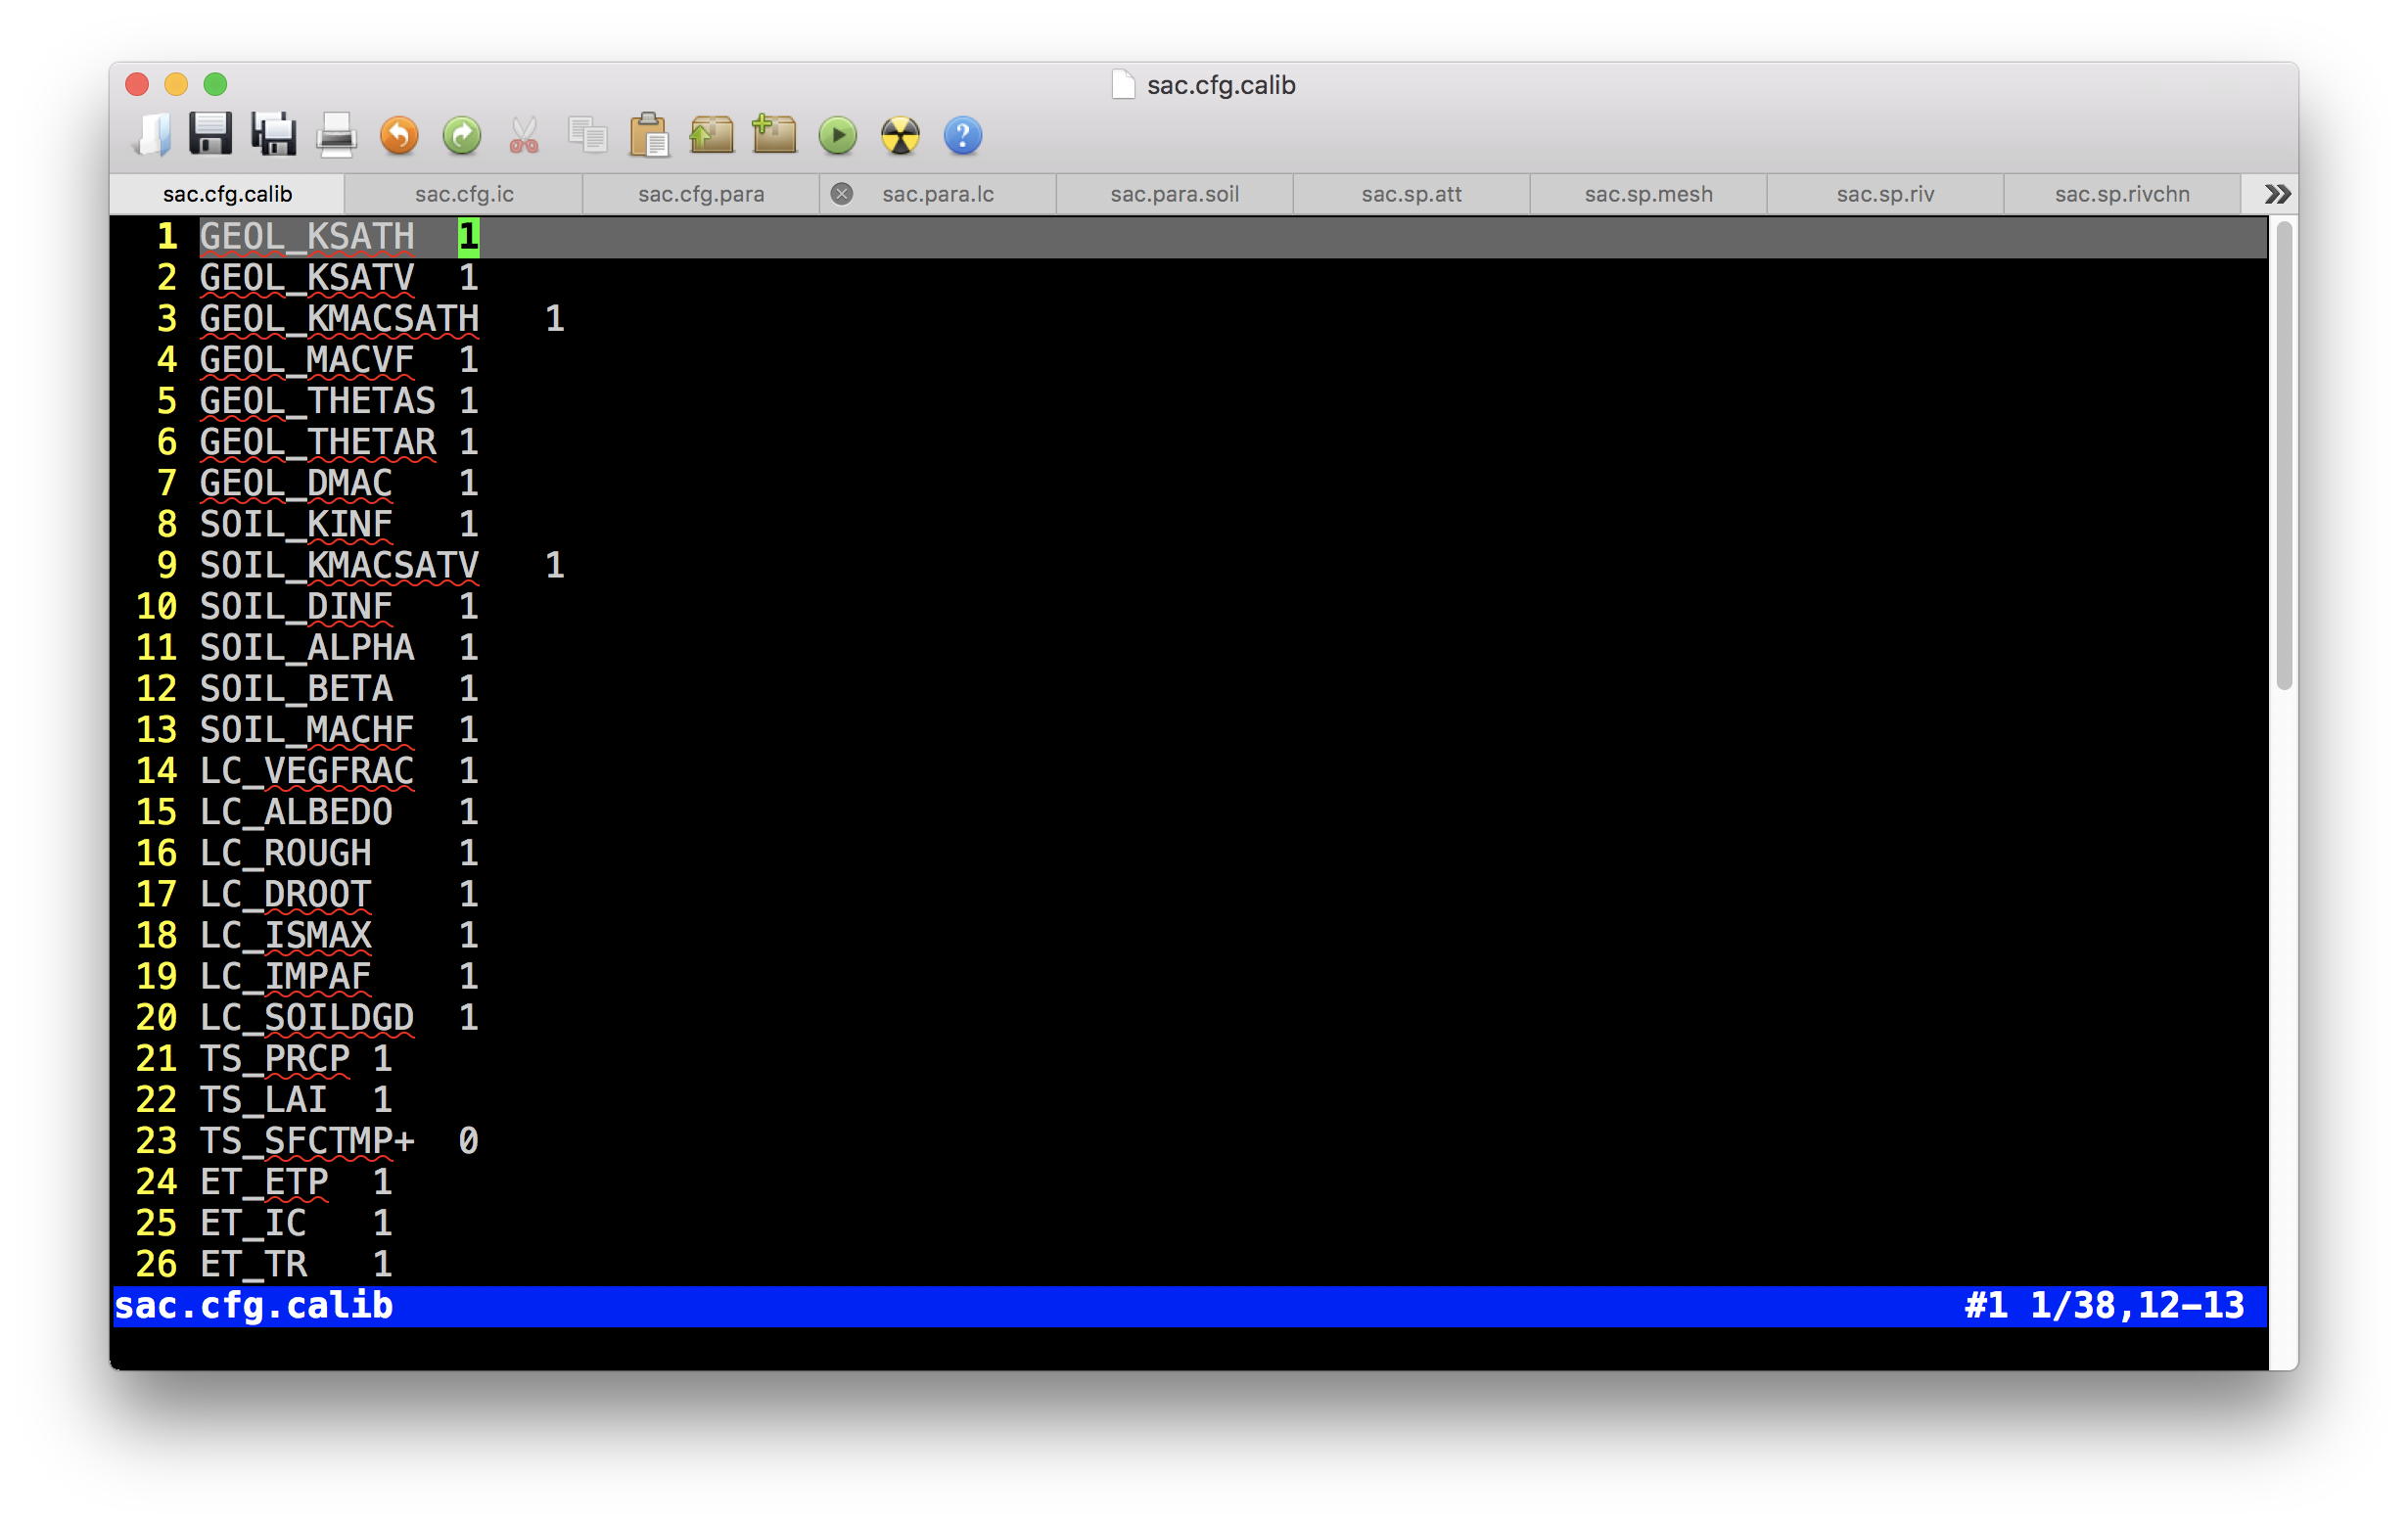
\includegraphics{Fig/IO/cfg.calib.png}
\caption{Example of .cfg.calib file}
\end{figure}

\begin{itemize}
\tightlist
\item
  Table
\end{itemize}

\begin{longtable}[]{@{}ccccc@{}}
\toprule
Colname & Meaning & Range & Unit & Comments\tabularnewline
\midrule
\endhead
GEOL\_KSATH & Horizontal conductivity of ground water & ? & -
&\tabularnewline
GEOL\_KSATV & Vertical conductivity of ground water & ? & -
&\tabularnewline
GEOL\_KMACSATH & Horizontal conductivity of macropore & ? & -
&\tabularnewline
GEOL\_DMAC & Macropore depth & & - &\tabularnewline
GEOL\_THETAS & Porosity, saturated soil moisture & & - &\tabularnewline
GEOL\_THETAR & Residual soil moisture & & - &\tabularnewline
GEOL\_MACVF & Vertical macropore areal fraction & & - &\tabularnewline
SOIL\_KINF & Vertical conductivity of top soil & ? & - &\tabularnewline
SOIL\_KMACSATV & Vertical conductivity of soil macropore & ? & -
&\tabularnewline
SOIL\_DINF & Infiltration depth & ? & - &\tabularnewline
SOIL\_DROOT & Root depth & & - &\tabularnewline
SOIL\_ALPHA & \(\alpha\) value in van Genuchten equation & & -
&\tabularnewline
SOIL\_BETA & \(\beta\) value in van Genuchten equation & & -
&\tabularnewline
SOIL\_MACHF & Horizontal macropore areal fraction & & - &\tabularnewline
LC\_VEGFRAC & Vegetation fraction & & - &\tabularnewline
LC\_ALBEDO & Emissitive reflection ratio & & - &\tabularnewline
LC\_ROUGH & Manning's roughness of cell surface & & - &\tabularnewline
LC\_SOILDGD & Soil degradation & & - &\tabularnewline
LC\_IMPAF & Impervious areal fraction & & - &\tabularnewline
LC\_ISMAX & Maximum interception & & - &\tabularnewline
AQ\_DEPTH+ & Thichness of aquifer & & \(m\) &\tabularnewline
TS\_PRCP & Precipitation & & - &\tabularnewline
TS\_SFCTMP+ & Temperature & & \(C\) &\tabularnewline
ET\_ETP & Transpiration & & - &\tabularnewline
ET\_IC & Interception & & - &\tabularnewline
ET\_TR & Evaporation & & - &\tabularnewline
ET\_SOIL & Evaporation & & - &\tabularnewline
RIV\_ROUGH & Manning's roughness of river & & - &\tabularnewline
RIV\_KH & Conductivity of river bed & & - &\tabularnewline
RIV\_DPTH+ & Depth of river cross section & & \(m\) &\tabularnewline
RIV\_WDTH+ & Width of river cross section & & \(m\) &\tabularnewline
RIV\_SINU & Sinuosity of river path & & - &\tabularnewline
RIV\_CWR & \(C_{wr}\) in Chezy equation & & - &\tabularnewline
RIV\_BSLOPE+ & Slope of river bed & & \(m/m\) &\tabularnewline
IC\_GW+ & Initial condition of groundwater & & \(m\) &\tabularnewline
IC\_RIV+ & Initial condition of river stage & & \(m\) &\tabularnewline
\bottomrule
\end{longtable}

\subsection{.cfg.ic file}\label{cfg.ic-file}

\begin{figure}
\centering
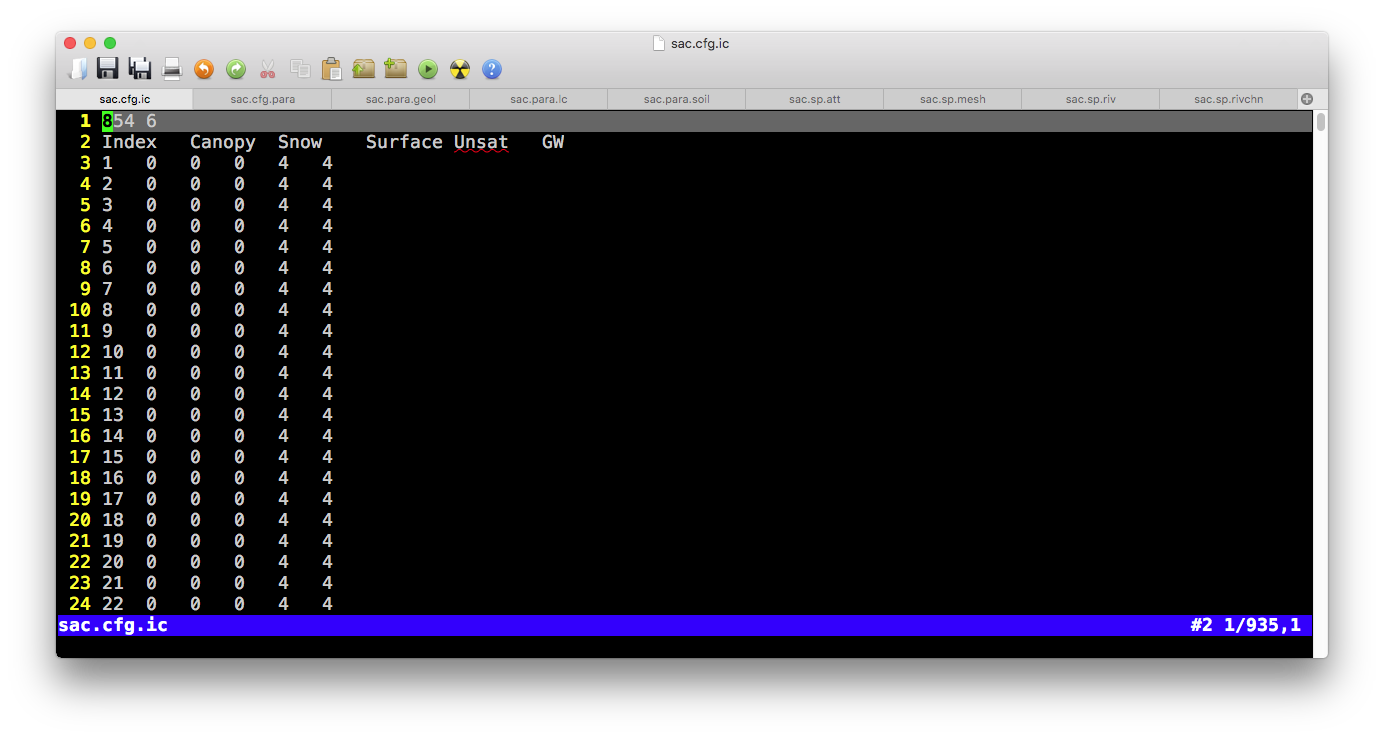
\includegraphics{Fig/IO/cfg.ic.png}
\caption{Example of .cfg.ic file}
\end{figure}

\begin{itemize}
\item
  \textbf{Block 1 (cell initial condition)}
\item
  Pre-table
\end{itemize}

\begin{longtable}[]{@{}cc@{}}
\toprule
Value1 & Value2\tabularnewline
\midrule
\endhead
Number of rows ( \(N_{cell}\)) & Number of columns
(\(6\))\tabularnewline
\bottomrule
\end{longtable}

\begin{itemize}
\tightlist
\item
  Table
\end{itemize}

\begin{longtable}[]{@{}ccccc@{}}
\toprule
Colname & Meaning & Range & Unit & Comments\tabularnewline
\midrule
\endhead
ID & Index of cell \(i\) & 1 \textasciitilde{} \(N_{cell}\) & -
&\tabularnewline
Canopy & Canopy storage of cell \(i\) & 0 \textasciitilde{} inf & \(m\)
&\tabularnewline
Snow & Snow storage of cell \(i\) & 0 \textasciitilde{} inf & \(m\)
&\tabularnewline
Surface & Surface storage of cell \(i\) & 0 \textasciitilde{} inf &
\(m\) &\tabularnewline
Unsat & Unsaturated storage of cell \(i\) & 0 \textasciitilde{} inf &
\(m\) &\tabularnewline
GW & Groundwater head of cell \(i\) & 0 \textasciitilde{} inf & \(m\)
&\tabularnewline
\bottomrule
\end{longtable}

\begin{itemize}
\item
  \textbf{Block 2 (river initial condition)}
\item
  Pre-table:
\end{itemize}

\begin{longtable}[]{@{}cc@{}}
\toprule
Value1 & Value2\tabularnewline
\midrule
\endhead
Number of rows ( \(N_{riv}\)) & Number of columns (\(2\))\tabularnewline
\bottomrule
\end{longtable}

\begin{itemize}
\tightlist
\item
  Table
\end{itemize}

\begin{longtable}[]{@{}ccccc@{}}
\toprule
Colname & Meaning & Range & Unit & Comments\tabularnewline
\midrule
\endhead
ID & Index of river \(i\) & 1 \textasciitilde{} \(N_{riv}\) & -
&\tabularnewline
Stage & Stage of river \(i\) & 0 \textasciitilde{} inf & \(m\)
&\tabularnewline
\bottomrule
\end{longtable}

\section{Time-series data}\label{time-series-data}

\subsection{.tsd.forc file}\label{tsd.forc-file}

\begin{figure}
\centering
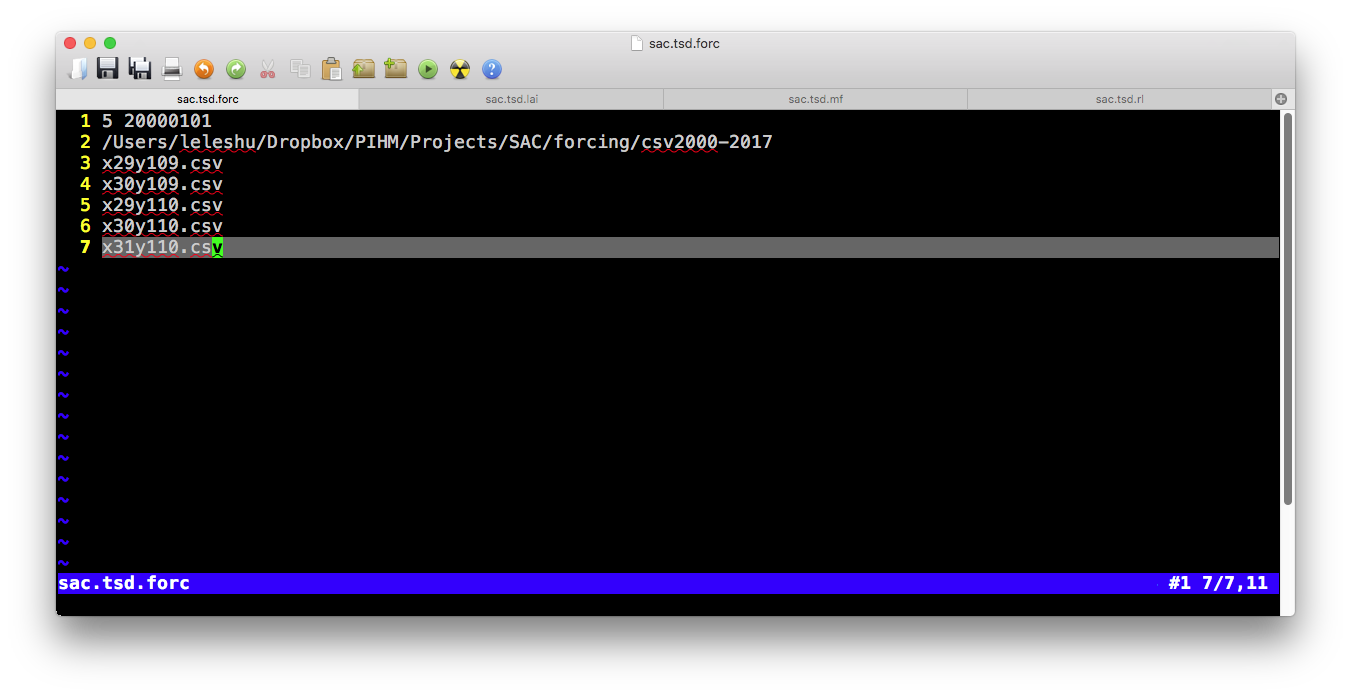
\includegraphics{Fig/IO/tsd.forc.png}
\caption{Example of .tsd.forc file}
\end{figure}

\begin{itemize}
\tightlist
\item
  Line 1:
  \texttt{Number\ of\ forcing\ sites\ \textbar{}\ Start\ day\ (YYYYMMDD)}
\item
  Line 2: Directory to the spreadsheet
\item
  Line 3\textasciitilde{}N: Filenames of spreadsheet
\end{itemize}

\begin{figure}
\centering
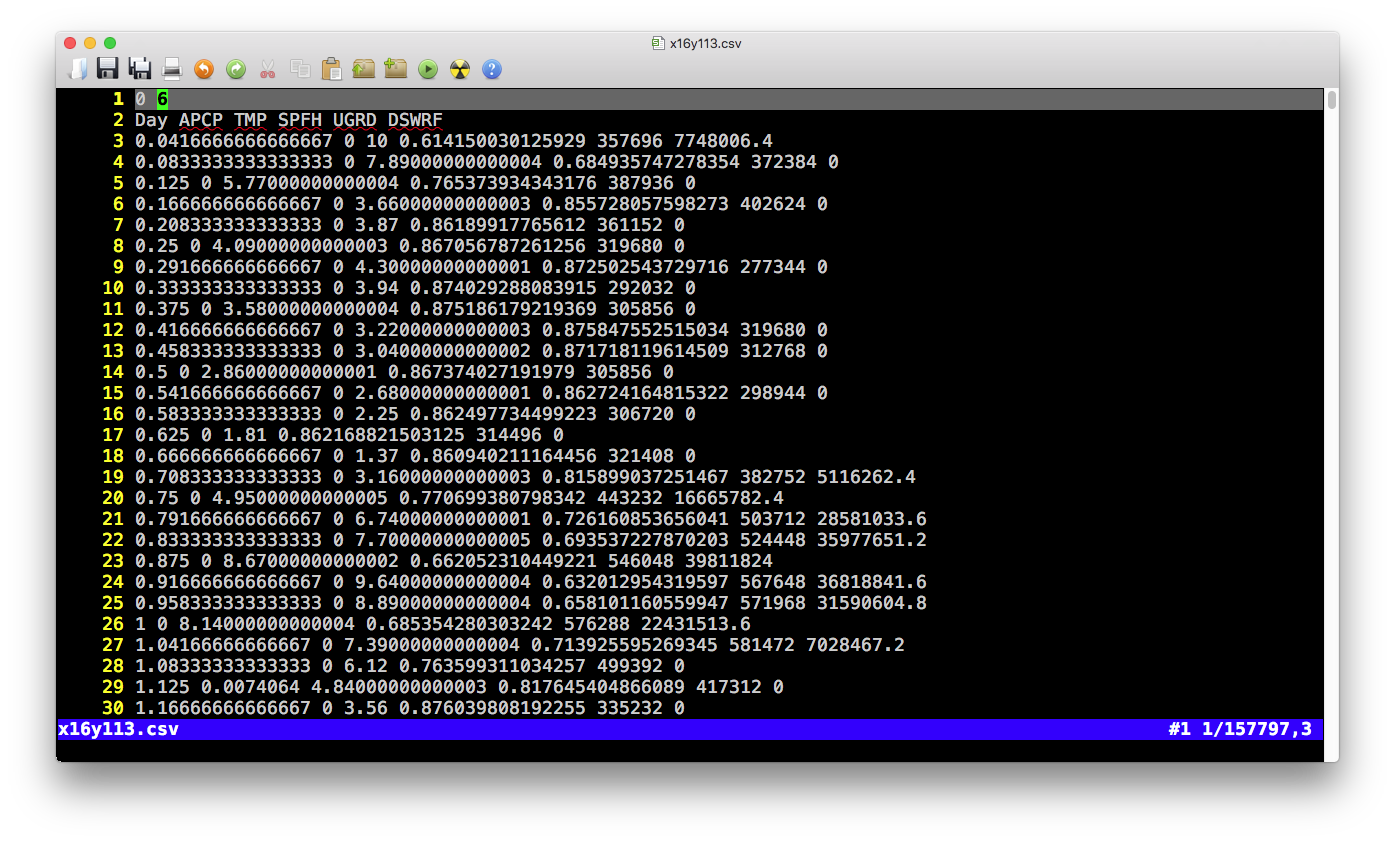
\includegraphics{Fig/IO/tsd.csv.png}
\caption{Example of .csv forcing file}
\end{figure}

\begin{itemize}
\tightlist
\item
  Pre-table:
\end{itemize}

\begin{longtable}[]{@{}cc@{}}
\toprule
Value1 & Value2\tabularnewline
\midrule
\endhead
( \(0\)) & Number of columns (\(6\))\tabularnewline
\bottomrule
\end{longtable}

\begin{itemize}
\tightlist
\item
  Table
\end{itemize}

\begin{longtable}[]{@{}ccccc@{}}
\toprule
Colname & Meaning & Range & Unit & Comments\tabularnewline
\midrule
\endhead
Day & Time & 0 \textasciitilde{} \(N_{day}\) & \(day\) &\tabularnewline
PRCP & Precipitation & 0 \textasciitilde{} 1 & \(m/day\)
&\tabularnewline
TEMP & Temperature & -100 \textasciitilde{} 70 & \(C\) &\tabularnewline
RH & Relative Humidity & 0 \textasciitilde{} 1 & \(-\) &\tabularnewline
wind & Wind Speed & 0 \textasciitilde{} inf & \(m/day\) &\tabularnewline
Rn & Solar (shortwave) radiation & ? & \(J/day/m^2\) &\tabularnewline
\bottomrule
\end{longtable}

\subsection{.tsd.lai file}\label{tsd.lai-file}

\begin{figure}
\centering
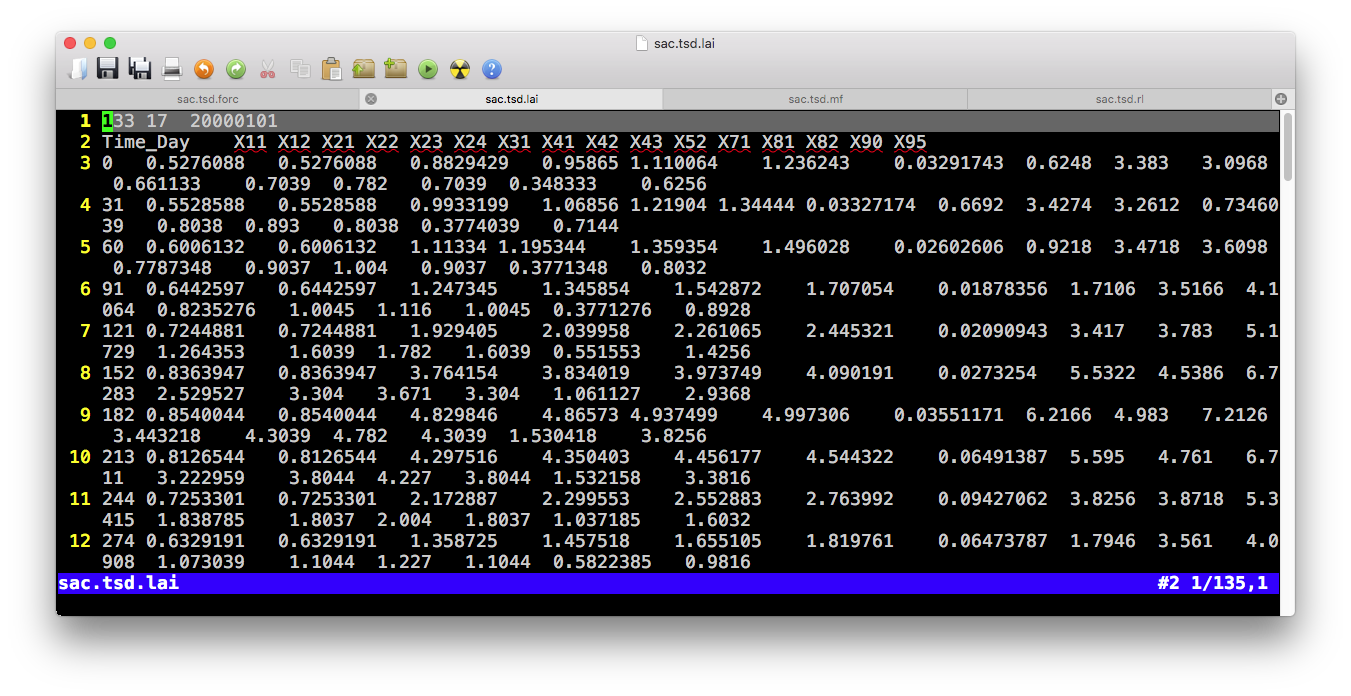
\includegraphics{Fig/IO/tsd.lai.png}
\caption{Example of .tsd.lai file}
\end{figure}

\begin{itemize}
\tightlist
\item
  Pre-table:
\end{itemize}

\begin{longtable}[]{@{}ccc@{}}
\toprule
Value1 & Value2 & Value3\tabularnewline
\midrule
\endhead
Number of day ( \(N_{time}\)) & Number of columns (\(N_{lc}\)) & Start
day (YYYYMMDD)\tabularnewline
\bottomrule
\end{longtable}

\begin{itemize}
\tightlist
\item
  Table
\end{itemize}

\begin{longtable}[]{@{}ccccc@{}}
\toprule
Colname & Meaning & Range & Unit & Comments\tabularnewline
\midrule
\endhead
TIME & Time & 0 \textasciitilde{} \(N_{time}\) & \(day\)
&\tabularnewline
Column 2 & LAI of land cover 1 & 0 \textasciitilde{} inf & \(m^2/m^2\)
&\tabularnewline
Column i & LAI of land cover \(i-1\) & 0 \textasciitilde{} inf &
\(m^2/m^2\) &\tabularnewline
\ldots{} & \ldots{} & \ldots{} & \ldots{} &\tabularnewline
\bottomrule
\end{longtable}

\subsection{.tsd.rl file}\label{tsd.rl-file}

\begin{figure}
\centering
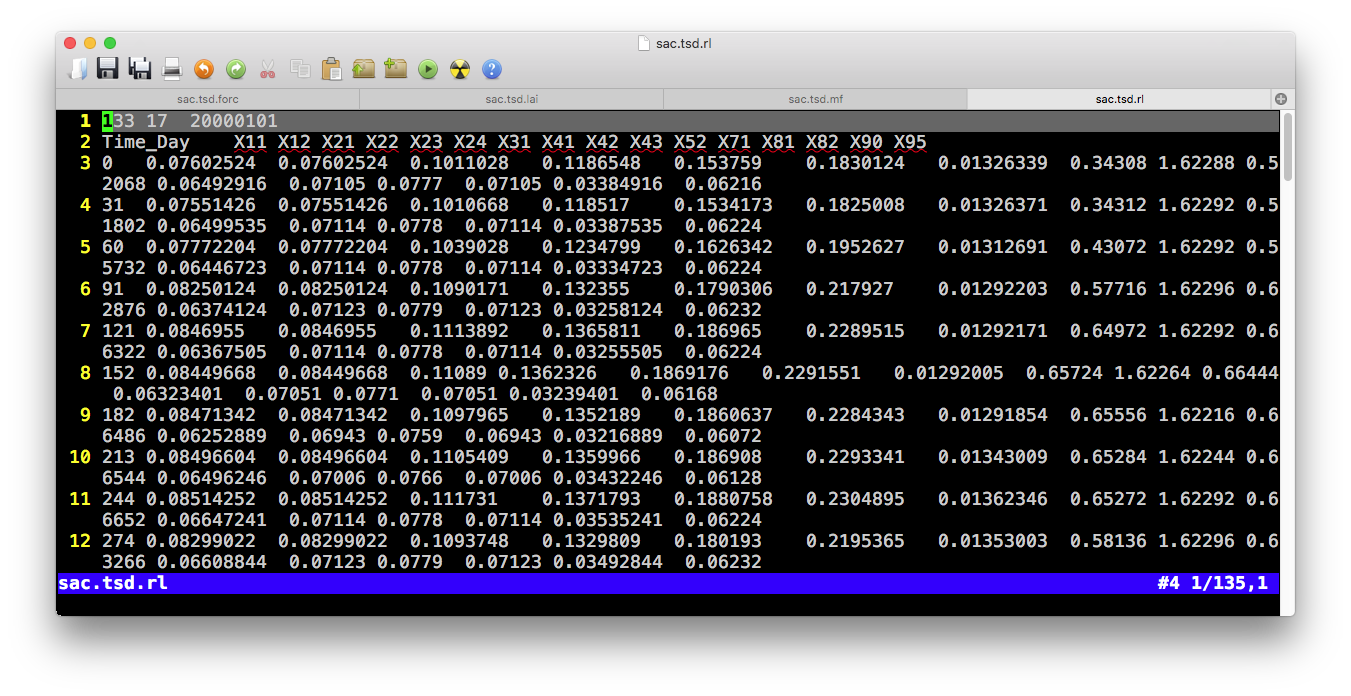
\includegraphics{Fig/IO/tsd.rl.png}
\caption{Example of .tsd.rl file}
\end{figure}

\begin{itemize}
\tightlist
\item
  Pre-table:
\end{itemize}

\begin{longtable}[]{@{}ccc@{}}
\toprule
Value1 & Value2 & Value3\tabularnewline
\midrule
\endhead
Number of day ( \(N_{time}\)) & Number of columns (\(N_{lc}\)) & Start
day (YYYYMMDD)\tabularnewline
\bottomrule
\end{longtable}

\begin{itemize}
\tightlist
\item
  Table
\end{itemize}

\begin{longtable}[]{@{}ccccc@{}}
\toprule
Colname & Meaning & Range & Unit & Comments\tabularnewline
\midrule
\endhead
TIME & Time & 0 \textasciitilde{} \(N_{time}\) & \(day\)
&\tabularnewline
Column 2 & Roughness length of land cover 1 & 0 \textasciitilde{} inf &
\(m\) &\tabularnewline
Column i & Roughness length of land cover \(i-1\) & 0 \textasciitilde{}
inf & \(m\) &\tabularnewline
\ldots{} & \ldots{} & \ldots{} & \ldots{} &\tabularnewline
\bottomrule
\end{longtable}

\subsection{.tsd.mf file}\label{tsd.mf-file}

\begin{figure}
\centering
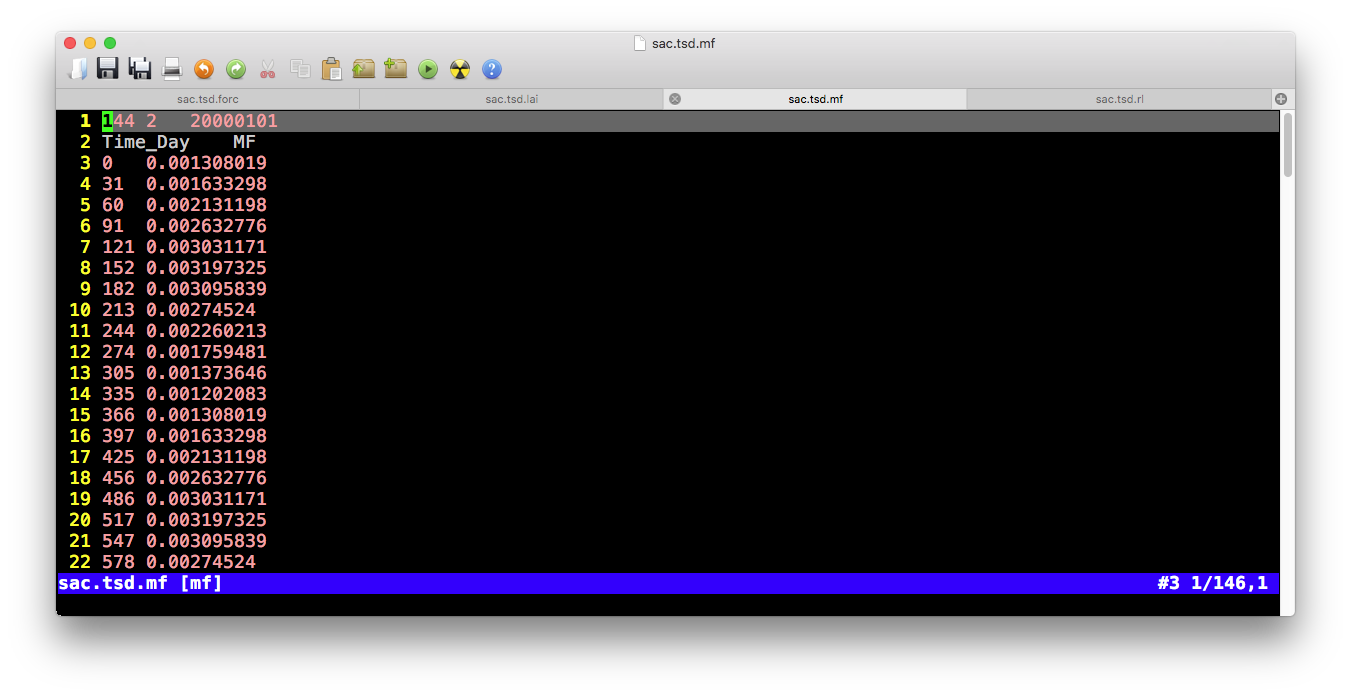
\includegraphics{Fig/IO/tsd.mf.png}
\caption{Example of .tsd.mf file}
\end{figure}

\begin{itemize}
\tightlist
\item
  Pre-table:
\end{itemize}

\begin{longtable}[]{@{}ccc@{}}
\toprule
Value1 & Value2 & Value3\tabularnewline
\midrule
\endhead
Number of day ( \(N_{time}\)) & Number of columns (\(N_{mf}\)) & Start
day (YYYYMMDD)\tabularnewline
\bottomrule
\end{longtable}

\begin{itemize}
\tightlist
\item
  Table
\end{itemize}

\begin{longtable}[]{@{}ccccc@{}}
\toprule
Colname & Meaning & Range & Unit & Comments\tabularnewline
\midrule
\endhead
TIME & Time & 0 \textasciitilde{} \(N_{time}\) & \(day\)
&\tabularnewline
Column 2 & Melt factor 1 & 0 \textasciitilde{} inf & - &\tabularnewline
Column i & Melt factor \(i-1\) & 0 \textasciitilde{} inf & -
&\tabularnewline
\ldots{} & \ldots{} & \ldots{} & \ldots{} &\tabularnewline
\bottomrule
\end{longtable}

\subsection{.tsd.obs file}\label{tsd.obs-file}

\begin{figure}
\centering
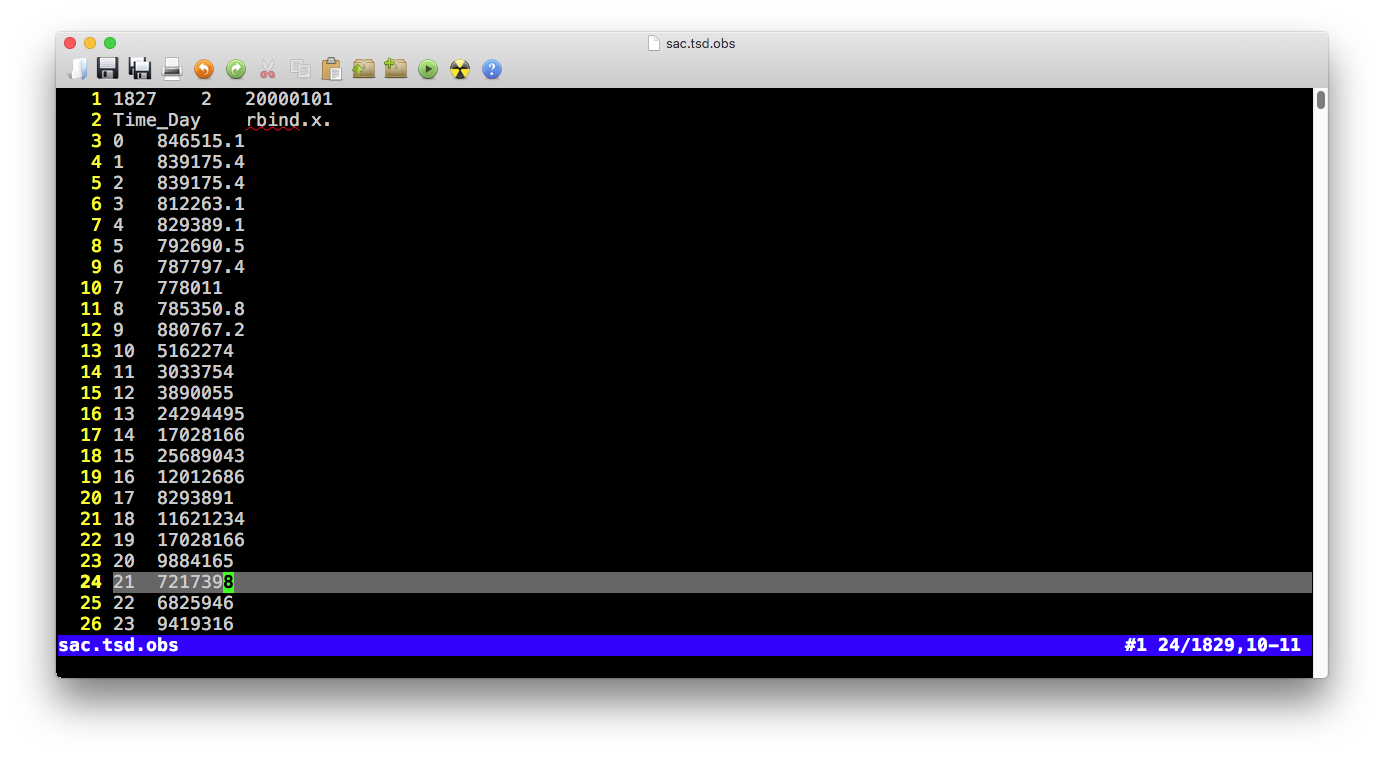
\includegraphics{Fig/IO/tsd.obs.png}
\caption{Example of .tsd.obs file}
\end{figure}

\begin{itemize}
\tightlist
\item
  Pre-table:
\end{itemize}

\begin{longtable}[]{@{}ccc@{}}
\toprule
Value1 & Value2 & Value3\tabularnewline
\midrule
\endhead
Number of day ( \(N_{time}\)) & Number of columns (\(N_{obs}\)) & Start
day (YYYYMMDD)\tabularnewline
\bottomrule
\end{longtable}

\begin{itemize}
\tightlist
\item
  Table
\end{itemize}

\begin{longtable}[]{@{}ccccc@{}}
\toprule
Colname & Meaning & Range & Unit & Comments\tabularnewline
\midrule
\endhead
TIME & Time & 0 \textasciitilde{} \(N_{time}\) & \(day\)
&\tabularnewline
Column 2 & Observational data 1 & ? & ? &\tabularnewline
Column i & Observational data \(i-1\) & ? & ? &\tabularnewline
\ldots{} & \ldots{} & \ldots{} & \ldots{} &\tabularnewline
\bottomrule
\end{longtable}

\chapter{Output files}\label{output-files}

\section{Output file names}\label{output-file-names}

Format of output file names:

\textbf{{[}Project Name{]}.{[}Identifier{]}.{[}Format{]}}

-The \emph{{[}Project Name{]}} is user defined name of the project, so
every input and output files must start with the \emph{{[}Project
Name{]}}. -The \emph{{[}Format{]}} is one of \emph{csv} or \emph{dat}.
\emph{csv} is spreadsheet format and \emph{dat} is bindary format.

The \emph{{[}Identifier{]}} is a combination of variables features, that
in format of: \textbf{{[}Model Unit{]}{[}Variable Type{]}{[}Variable
Name{]}}. \emph{{[}Model Unit{]}} is one of three options of \emph{ele}
(elemtns), \emph{riv} (river) or \emph{lak} (lake). Variable type
includes \emph{y}, \emph{v} and \emph{q} that are state variable (in
\(L\)), specific flux (in \(L^3/L^2/T\)) and flux (in \(L^3/T\))
respectively.

The list of output files is in following table.

\begin{longtable}[]{@{}ccccccc@{}}
\toprule
Identifier & Mod unit & Type & Var Name & Meaning & Unit\tabularnewline
\midrule
\endhead
\emph{.eleyic.} & ele & y & ic & Storage of Interception & \(m\)
&\tabularnewline
\emph{.eleysnow.} & ele & y & snow & Storage of snow equivalence & \(m\)
&\tabularnewline
\emph{.eleysurf.} & ele & y & surf & Storage of surface & \(m\)
&\tabularnewline
\emph{.eleyunsat.} & ele & y & unsat & Storage of vados zone & \(m\)
&\tabularnewline
\emph{.eleygw.} & ele & y & gw & Groundwater head & \(m\) &
.GW\tabularnewline
\emph{.elevetp.} & ele & v & etp & Potential ET & \(\frac{m^3}{m^2 d}\)
&\tabularnewline
\emph{.eleveta.} & ele & v & eta & Actual ET & \(\frac{m^3}{m^2 d}\)
&\tabularnewline
\emph{.elevetic.} & ele & v & etic & Evap of interception &
\(\frac{m^3}{m^2 d}\) &\tabularnewline
\emph{.elevettr.} & ele & v & ettr & Transpiration &
\(\frac{m^3}{m^2 d}\) &\tabularnewline
\emph{.elevetev.} & ele & v & etev & Soil Evaporation &
\(\frac{m^3}{m^2 d}\) &\tabularnewline
\emph{.elevprcp.} & ele & v & prcp & Precipitation &
\(\frac{m^3}{m^2 d}\) &\tabularnewline
\emph{.elevnetprcp.} & ele & v & netprcp & Net Precipitation &
\(\frac{m^3}{m^2 d}\) &\tabularnewline
\emph{.elevinfil.} & ele & v & infil & Infiltration Rate &
\(\frac{m^3}{m^2 d}\) &\tabularnewline
\emph{.elevexfil.} & ele & v & infil & Exfiltration Rate &
\(\frac{m^3}{m^2 d}\) &\tabularnewline
\emph{.elevrech.} & ele & v & rech & Recharge Rate &
\(\frac{m^3}{m^2 d}\) &\tabularnewline
\emph{.eleqsurf.} & ele & q & surf & Overland flow & \(m^3/d\)
&\tabularnewline
\emph{.eleqsub.} & ele & q & sub & Subsurface flow & \(m^3/d\)
&\tabularnewline
\emph{.rivystage.} & riv & y & stage & River Stage & \(m\)
&\tabularnewline
\emph{.rivqup.} & riv & q & up & Flux to upstream & \(m^3/d\)
&\tabularnewline
\emph{.rivqdown.} & riv & q & down & Flux to downstream & \(m^3/d\)
&\tabularnewline
\emph{.rivqsurf.} & riv & q & surf & Flux to landsurface & \(m^3/d\)
&\tabularnewline
\emph{.rivqsub.} & riv & q & sub & Flux to subsurface & \(m^3/d\)
&\tabularnewline
\bottomrule
\end{longtable}

\section{Data format in ASCII (.csv)
file}\label{data-format-in-ascii-.csv-file}

N - Number of column of output data, excluding the time column. m -
Number of time-step. StartTime - String of date/time (YYYYMMDD or
YYYYMMDD.hhmmss)

\begin{longtable}[]{@{}cccccc@{}}
\toprule
N & StartTime & & & &\tabularnewline
\midrule
\endhead
\(T_1\) & \(v_{1 \cdot 1}\) & \(v_{1 \cdot 2}\) & \ldots{} &
\(v_{1 \cdot N}\) &\tabularnewline
\(T_2\) & \(v_{2 \cdot 1}\) & \(v_{2 \cdot 2}\) & \ldots{} &
\(v_{2 \cdot N}\) &\tabularnewline
\(T_3\) & \(v_{3 \cdot 1}\) & \(v_{3 \cdot 2}\) & \ldots{} &
\(v_{3 \cdot N}\) &\tabularnewline
\ldots{} & \ldots{} & \ldots{} & \ldots{} & \ldots{} &\tabularnewline
\(T_{m}\) & \(v_{m \cdot 1}\) & \(v_{m \cdot 2}\) & \ldots{} &
\(v_{m \cdot N}\) &\tabularnewline
\bottomrule
\end{longtable}

\section{Data format in binary (.dat)
file}\label{data-format-in-binary-.dat-file}

The value saved in binary file are identical from ASCII format, but
different data structure.

\begin{longtable}[]{@{}ccccc@{}}
\toprule
ID & \(i\) & Value & Format & Length\tabularnewline
\midrule
\endhead
1 & - & \(N\) & double & 8\tabularnewline
2 & - & StartTime & double & 8\tabularnewline
3 & 0 & \(T_1\) & double & 8\tabularnewline
4 & 1 & \(v_{1 \cdot 1}\) & double & 8\tabularnewline
5 & 2 & \(v_{1 \cdot 2}\) & double & 8\tabularnewline
\ldots{} & \ldots{} & \ldots{} & double & 8\tabularnewline
\((N+1) * (T-1) + i +3\) & N & \(v_{1 \cdot N}\) & double &
8\tabularnewline
\((N+1) * (T-1) + i +3\) & 0 & \(T_2\) & double & 8\tabularnewline
\((N+1) * (T-1) + i +3\) & 1 & \(v_{2 \cdot 1}\) & double &
8\tabularnewline
\((N+1) * (T-1) + i +3\) & 2 & \(v_{2 \cdot 2}\) & double &
8\tabularnewline
\((N+1) * (T-1) + i +3\) & \ldots{} & \ldots{} & double &
8\tabularnewline
\((N+1) * (T-1) + i +3\) & N & \(v_{2 \cdot N}\) & double &
8\tabularnewline
\((N+1) * (T-1) + i +3\) & 0 & \(T_3\) & double & 8\tabularnewline
\((N+1) * (T-1) + i +3\) & 1 & \(v_{3 \cdot 1}\) & double &
8\tabularnewline
\((N+1) * (T-1) + i +3\) & 2 & \(v_{3 \cdot 2}\) & double &
8\tabularnewline
\((N+1) * (T-1) + i +3\) & \ldots{} & \ldots{} & double &
8\tabularnewline
\((N+1) * (T-1) + i +3\) & N & \(v_{3 \cdot N}\) & double &
8\tabularnewline
\((N+1) * (T-1) + i +3\) & \ldots{} & \ldots{} & double &
8\tabularnewline
\((N+1) * (T-1) + i +3\) & \ldots{} & \ldots{} & double &
8\tabularnewline
\((N+1) * (T-1) + i +3\) & \ldots{} & \ldots{} & double &
8\tabularnewline
\((N+1) * (T-1) + i +3\) & \ldots{} & \ldots{} & double &
8\tabularnewline
\((N+1) * (m-1) + i +3\) & 0 & \(T_{m}\) & double & 8\tabularnewline
\((N+1) * (m-1) + i +3\) & 1 & \(v_{m \cdot 1}\) & double &
8\tabularnewline
\((N+1) * (m-1) + i +3\) & 2 & \(v_{m \cdot 2}\) & double &
8\tabularnewline
\((N+1) * (m-1) + i +3\) & \ldots{} & \ldots{} & double &
8\tabularnewline
\((N+1) * (m-1) + i +3\) & N & \(v_{m \cdot N}\) & double &
8\tabularnewline
\bottomrule
\end{longtable}

\chapter{Applications}\label{applications}

Some \emph{significant} applications are demonstrated in this chapter.

\textbf{Best practice suggestions} 1. Derive and QC all inputs (time
mean, accumulation, screen fo anormalies \ldots{}) 1. Conduct offline
simulations \ldots{} 1. Start with `idealized' forcing (Option
FORC\_debug=1 in .cfg.para file). Which will use uniform forcing data to
drive the hydrologic simulations. 1. Run with short time period, load
the outputs and examine whether results are in expection 1. If all above
works, then hook all modules and run with your forcing data.

\section{Example 1: V-Catchment}\label{example-1-v-catchment}

Code annd data are available at
\href{https://zenodo.org/badge/latestdoi/226266189}{\includegraphics{https://zenodo.org/badge/226266189.svg}}
or
\href{https://github.com/Model-Intercomparison-Datasets/V-Catchment}{Github:
https://github.com/Model-Intercomparison-Datasets/V-Catchment}

The V-Catchment (VC) experiment is a standard test case for numerical
hydrological models to validate their performance for overland flow
along a hillslope and in the presence of a river channel. The VC domain
consists of two inclined planes draining into a sloping channel.

\begin{figure}
\centering
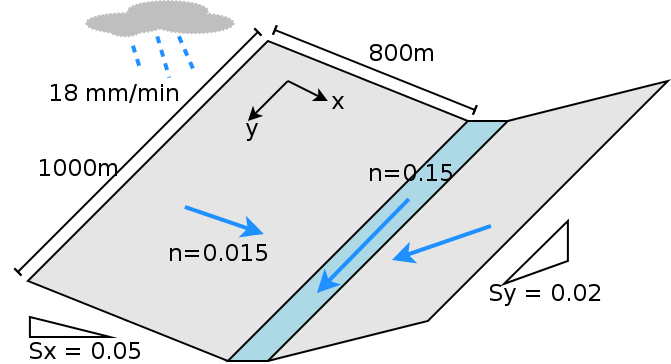
\includegraphics{Fig/Example/vCat/Vcat.png}
\caption{Description of the V-Catchmenet}
\end{figure}

Both hillslopes are \(800 \times 1000 m\) with Manning's roughness
\(n=0.015\). The river channel between the hillslopes is \(20\) m wide
and \(1000\) m in length with \(n=0.15\). The slope from the ridge to
the river channel is 0.05 (in the \(x\) direction), and the longitudinal
slope (in the \(y\) direction) is 0.02.

Rainfall in the VC begins at time zero at a constant rate of
\(18 mm/hr\) and stops after 90 min, producing \(27\) mm of accumulated
precipitation. Since evaporation and infiltration is not involved in
this simulation, the total outflow from lateral boundaries and the river
outlet must be the same as the total precipitation (following
conservation of mass).

\subsection{Shen(2010) result}\label{shen2010-result}

I use SHUD model to repeat the VC experiment, there are several
literatures did the same experiment, but only Shen(2010) export the flux
on side-plane which is also useful to validate the modeling algorithm.

\begin{figure}
\centering
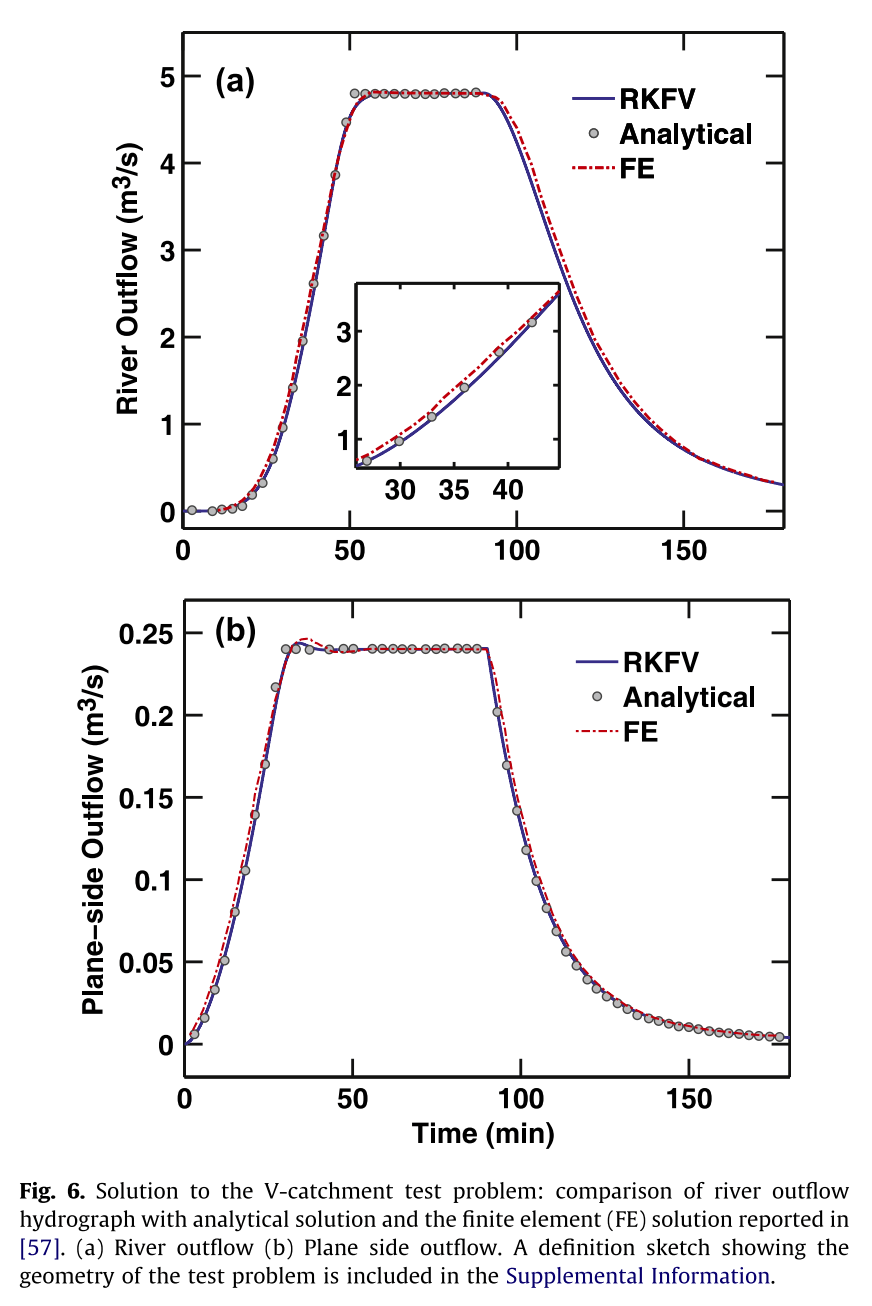
\includegraphics{Fig/Example/vCat/Shen2010.png}
\caption{Shen (2010) results}
\end{figure}

However, the value of volume flux of side-plane in Shen(2010) is
problematic. Lets explain: based on the Continuity Law, the total input
(precipitation) must be equal to output (side-plane flow) or discharge
(outlet flow). But the side-plane flux in Shen (2010) is 20 times less
than the discharge. I assume Shen made a wrong unit conversion somehow.
When I enlarge the side-plane flux by 20, the flux rate and accumulated
flux are rational. I tried to contact Shen, but he didn't reply with
explanation, so I continue the work with my understanding.

\begin{figure}
\centering
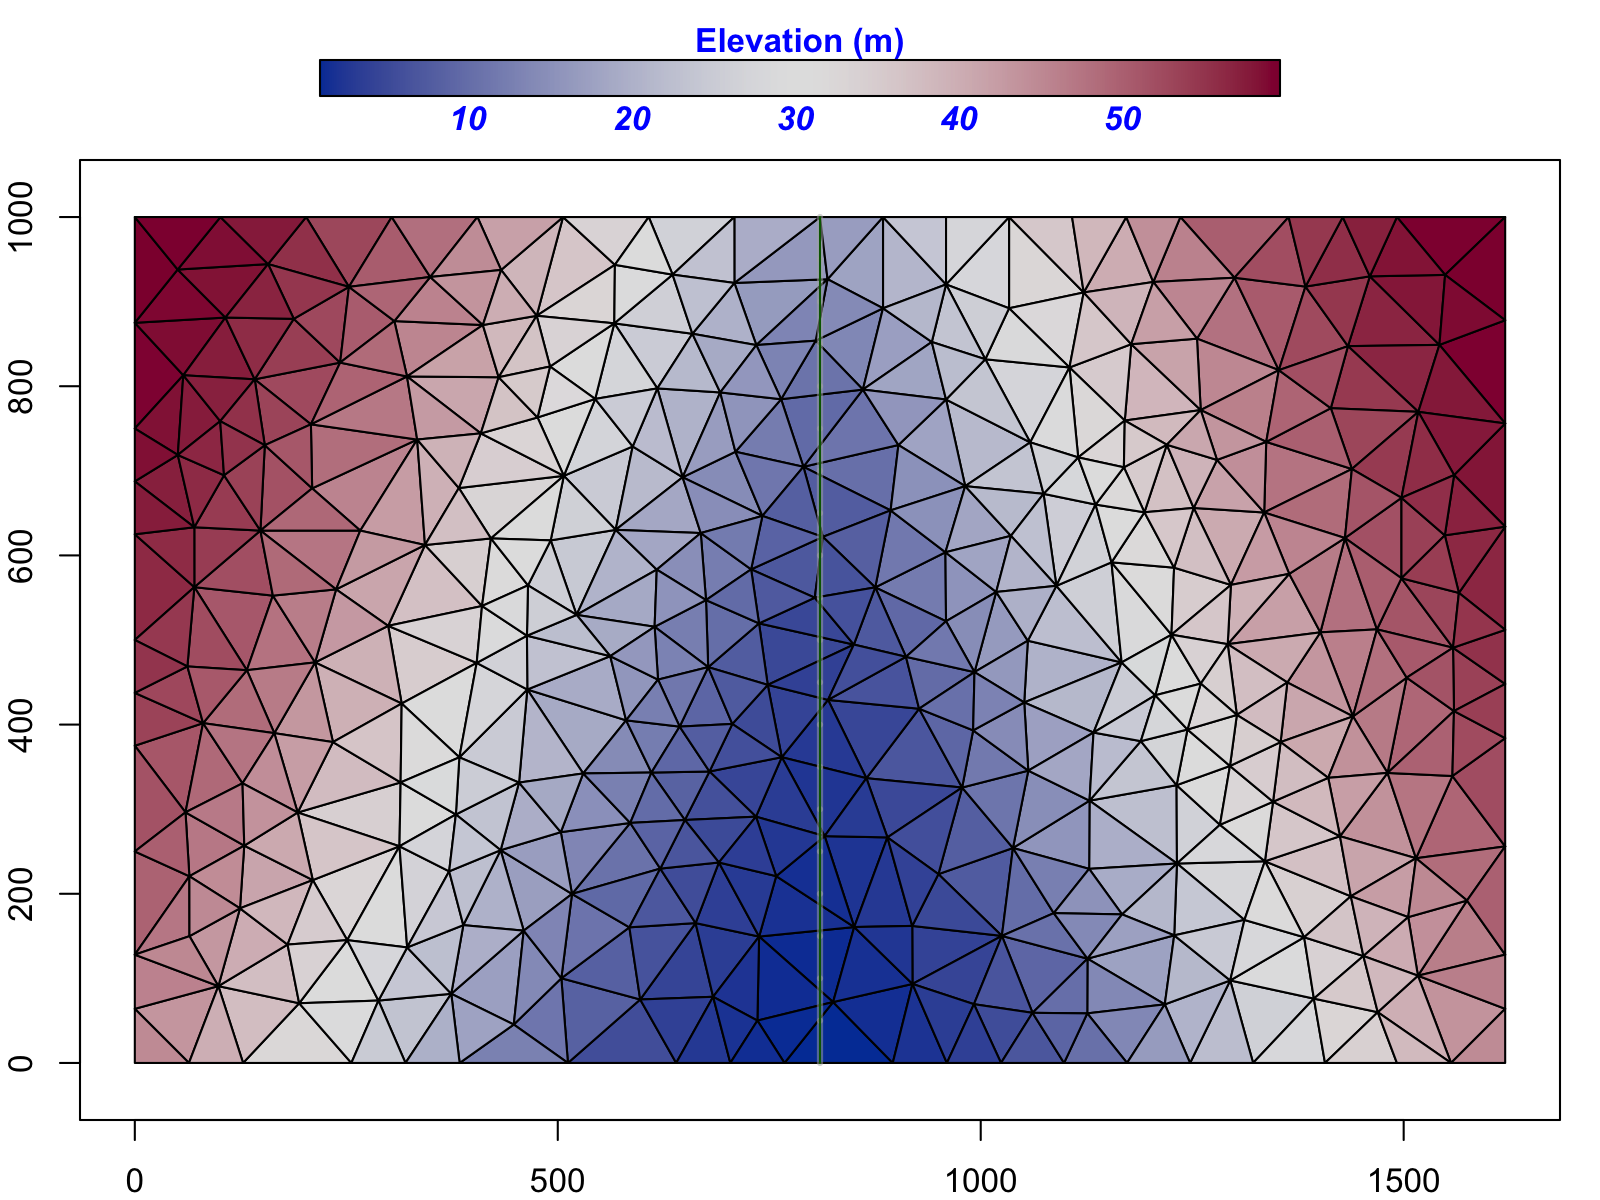
\includegraphics{Fig/Example/vCat/vc_mesh.png}
\caption{SHUD triangular model domain in V-Catchment}
\end{figure}

The result figure below also supports my thought. The side-plane flux in
the result figure is the modified value (Shen's side-plane flux times
20). Both flow rate meet the Continuity Law. So, I think this is the
right interpretation of Shen's result.

\begin{figure}
\centering
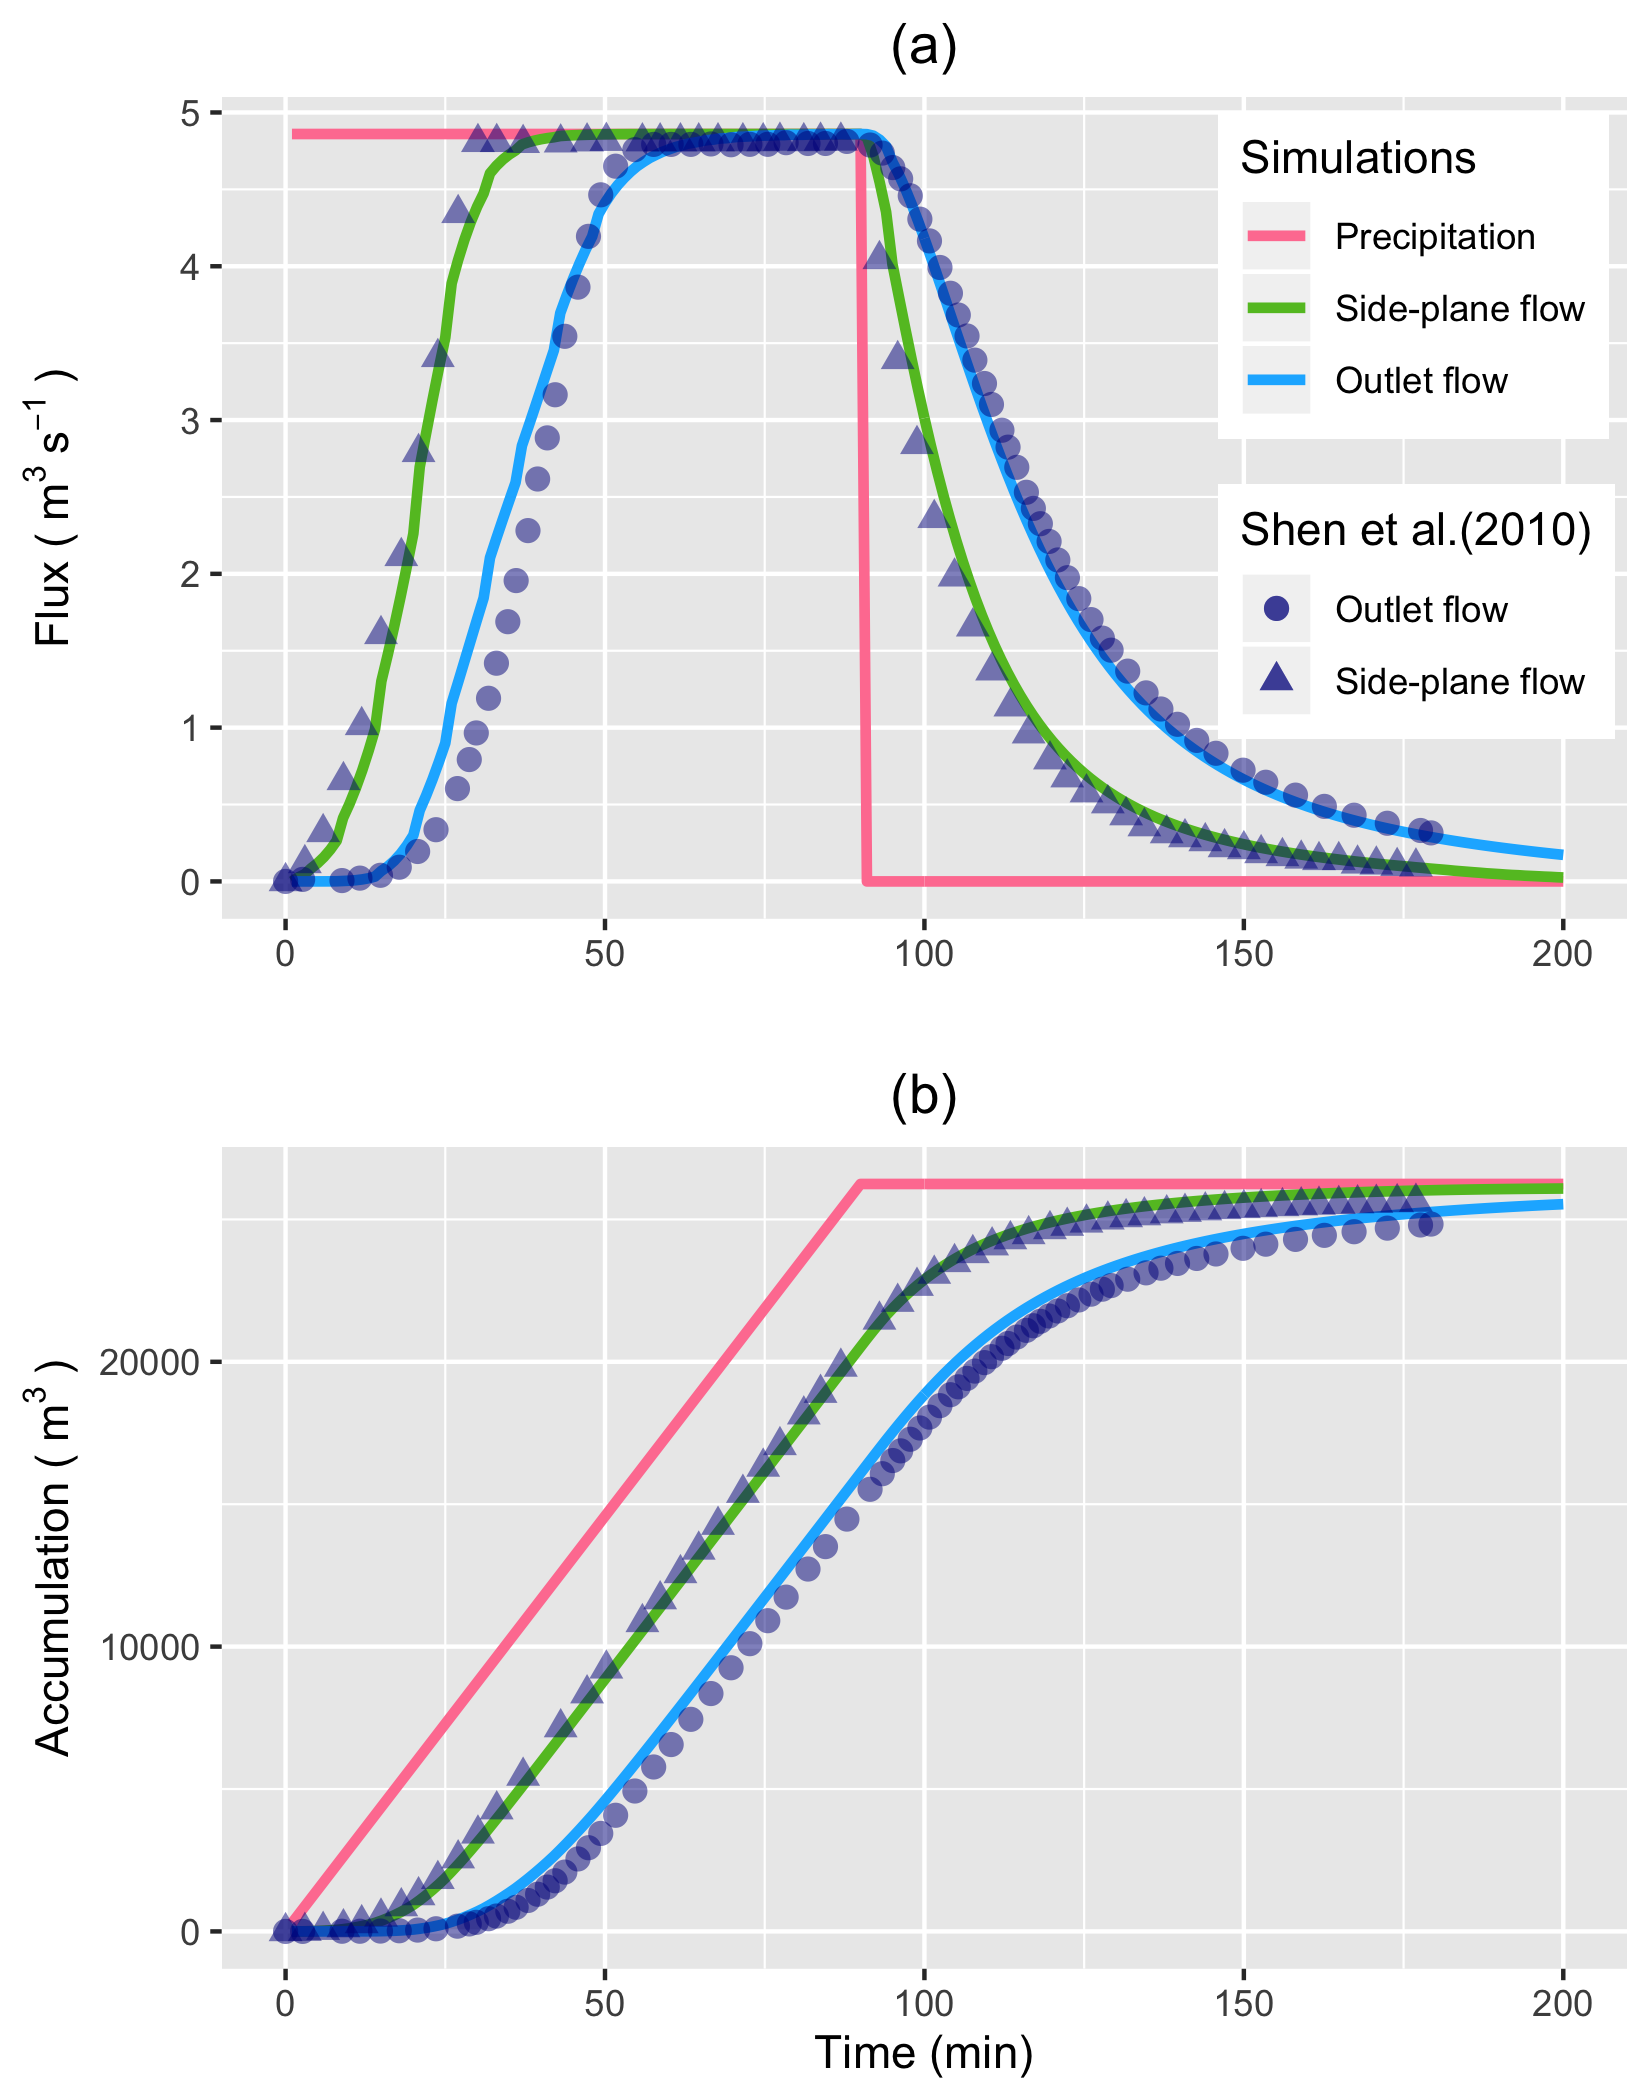
\includegraphics{Fig/Example/vCat/vcat_vs_vs.png}
\caption{Comparizon of SHUD modeling results versus Shen (2010).}
\end{figure}

\section{Example 2: Vauclin
Experiment}\label{example-2-vauclin-experiment}

Code annd data are available at
\href{https://zenodo.org/badge/latestdoi/226266864}{\includegraphics{https://zenodo.org/badge/226266864.svg}}
or
\href{https://github.com/Model-Intercomparison-Datasets/Vauclin1979}{Github:
https://github.com/Model-Intercomparison-Datasets/Vauclin1979}.

Vauclin's experiment \citep{Vauclin1979} is designed to assess
groundwater table change and soil moisture in the unsaturated layer
under precipitation or irrigation. The experiment was conducted in a
sandbox with dimension \(3\) m long \(\times 2\) m deep \(\times 0.05\)
m wide (see Fig. \ref{fig:vauclin}). The box was filled with uniform
sand particles with measured hydraulic parameters: the saturated
hydraulic conductivity was \(35\) cm/hr and porosity was \(0.33\)
m\(^3\)/m\(^3\). The left and bottom of the sandbox were impervious
layers, and the top and the right side were open. A hydraulic head was
set constant at \(0.65 m\). Constant irrigation (\(1.48\) cm/hr) was
applied over the first \(50\) cm of the top-left of the sandbox while
the rest of the top was covered to avoid water loss via evaporation.

\begin{figure}
\centering
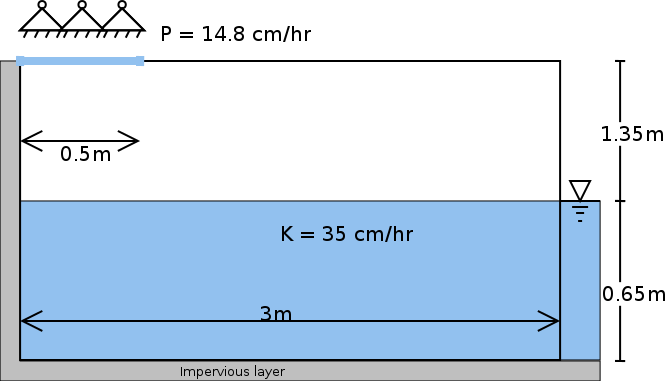
\includegraphics{Fig/Example/Vauclin/Vauclin.png}
\caption{Experiment set-up in Vauclin (1979)}
\end{figure}

\begin{figure}
\centering
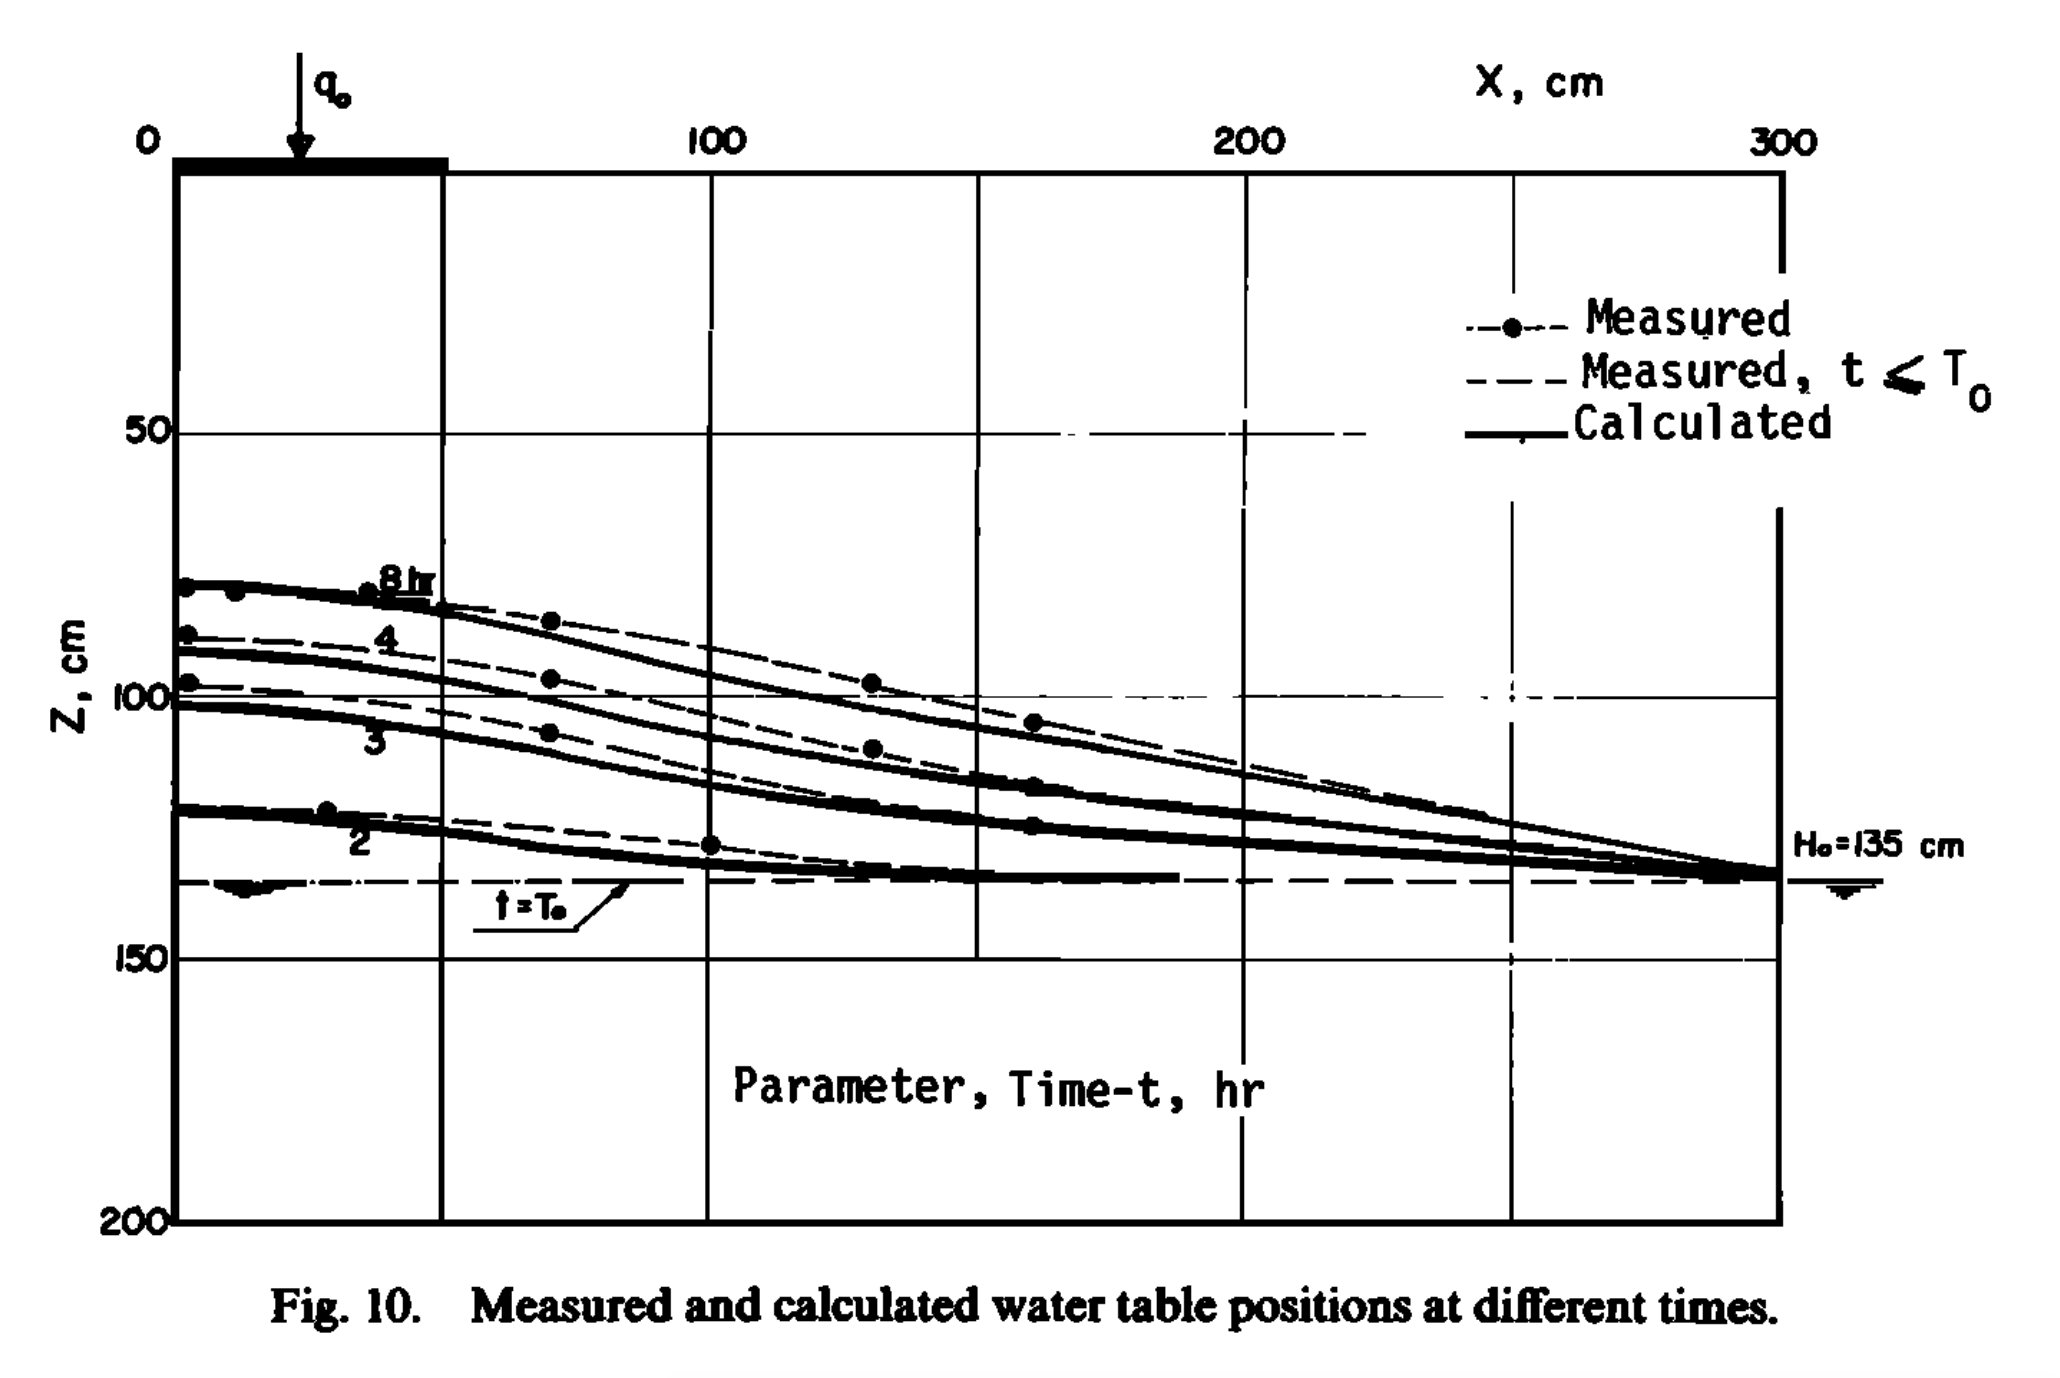
\includegraphics{Fig/Example/Vauclin/v1.png}
\caption{Groundwater measurement and 2-D numeric simulation in Vauclin
(1979)}
\end{figure}

The experiment's initial condition is an equilibrium water table under
constant hydraulic head from the right side. That is, the saturated
water table across the sandbox was kept stable at \(0.65\) m. When the
groundwater table reached equilibrium, irrigation was initiated at
\(t = 0\). The groundwater table was then measured at 2, 4, 6, and 8
hours at several locations along the length of the box.

\begin{figure}
\centering
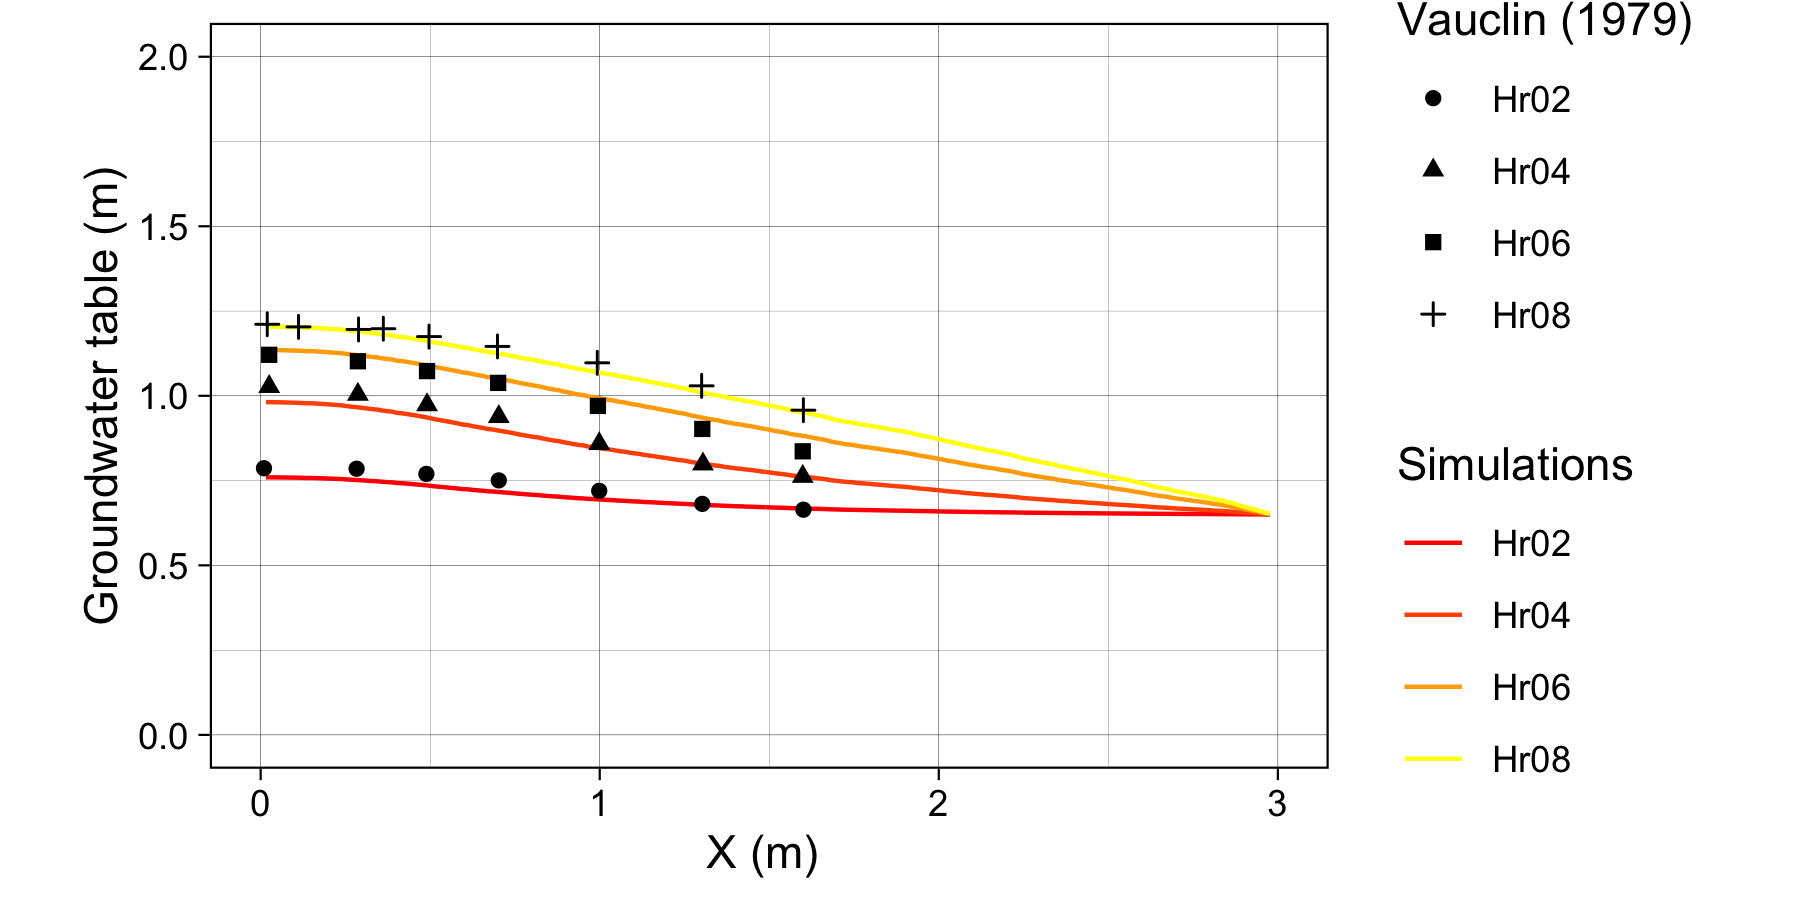
\includegraphics{Fig/Example/Vauclin/best.png}
\caption{Simulation results from SHUD model versus Vauclin (1979)
measurement}
\end{figure}

\citep{Vauclin1979} also use 2-D (vertical and horizontal) numeric model
to simulate the soil moisture and groundwater table. The maximum bias
between measurement and simulation was \$5.2 cm \$, according to the
value of digitalized in \citealp[Fig. 10]{Vauclin1979}.

Besides the parameters specified in \citep{Vauclin1979}, additional
information is needed by the SHUD, including the \(\alpha\) and
\(\beta\) in the van Genutchen equation and water content
(\(\theta _s\)). Therefore, we use a calibration tool to estimate the
representative values of these parameters. The use of calibration in
this simulation is reasonable because the model -- inevitably --
simplifies the real hydraulic processes. The calibration thus nudges the
parameters to \emph{representative} values that approach or fit the
\emph{true} natural processes. The calibrated values are
\(\theta _s = 0.32 m^3/m^3\), \(\alpha = 6.0\) and \(\beta = 6.0\). Like
the simulated results in \citep{Vauclin1979} and \citep{Shen2010}, a
mismatch exists between the simulations and measurements.

This mismatch may be due to (1) the aquifer description of unsaturated
and saturated layers limiting the capability to simulate infiltration
and recharge in the unsaturated zone, or (2) the horizontal unsaturated
flow assumptions no longer hold at the relatively microscopic scales of
this experiment.

The SHUD simulated the groundwater table at all four measurement points
(see Fig. \ref{fig:vauclin}(b). The maximum bias between simulation and
Vauclin's observations is \$ 5.5cm\$, with \(R^2\) = \(0.99\), that is
comparable to the bias \(5.2 cm\) of numerical simulation in
\citep{Vauclin1979}. When the calibration takes more soil parameters
into account, the bias in simulation decreases to \(3 cm\). Certainly,
the simplifications employed by SHUD for the unsaturated and saturated
zone benefits the computation efficiency while limiting the
applicability of the model for micro-scale problems.

The simulations, compared against Vauclin's experiment, validate the
algorithm for infiltration, recharge, and lateral groundwater flow. More
reliable vertical flow within unsaturated layer requires multiple
layers, which is planned in next version of SHUD.

\section{Example 3: Cache Creek
Watershed}\label{example-3-cache-creek-watershed}

Code is available at
\href{https://zenodo.org/badge/latestdoi/226413148}{\includegraphics{https://zenodo.org/badge/226413148.svg}}
and
\href{https://github.com/Model-Intercomparison-Datasets/Cache-Creek}{Github:
https://github.com/Model-Intercomparison-Datasets/Cache-Creek}. The data
is big. If you need, please email to
\href{mailto:lele.shu@gmail.com}{Lele Shu}

\subsection{Cache Creek Watershed}\label{cache-creek-watershed}

The Cache Creek Watershed (CCW) is a headwater catchment with area
\(196.4 km^2\) in the Sacramento Watershed in Northern California
(Figures \ref{fig:sh} (a), (b) and (c)). The elevation ranges from
\(450 m\) to \(1800 m\), with a \(0.38 m/m\) average slope which is very
steep, and hence a particularly difficult watershed for hydrologic
models to simulate.

\begin{figure}
\centering
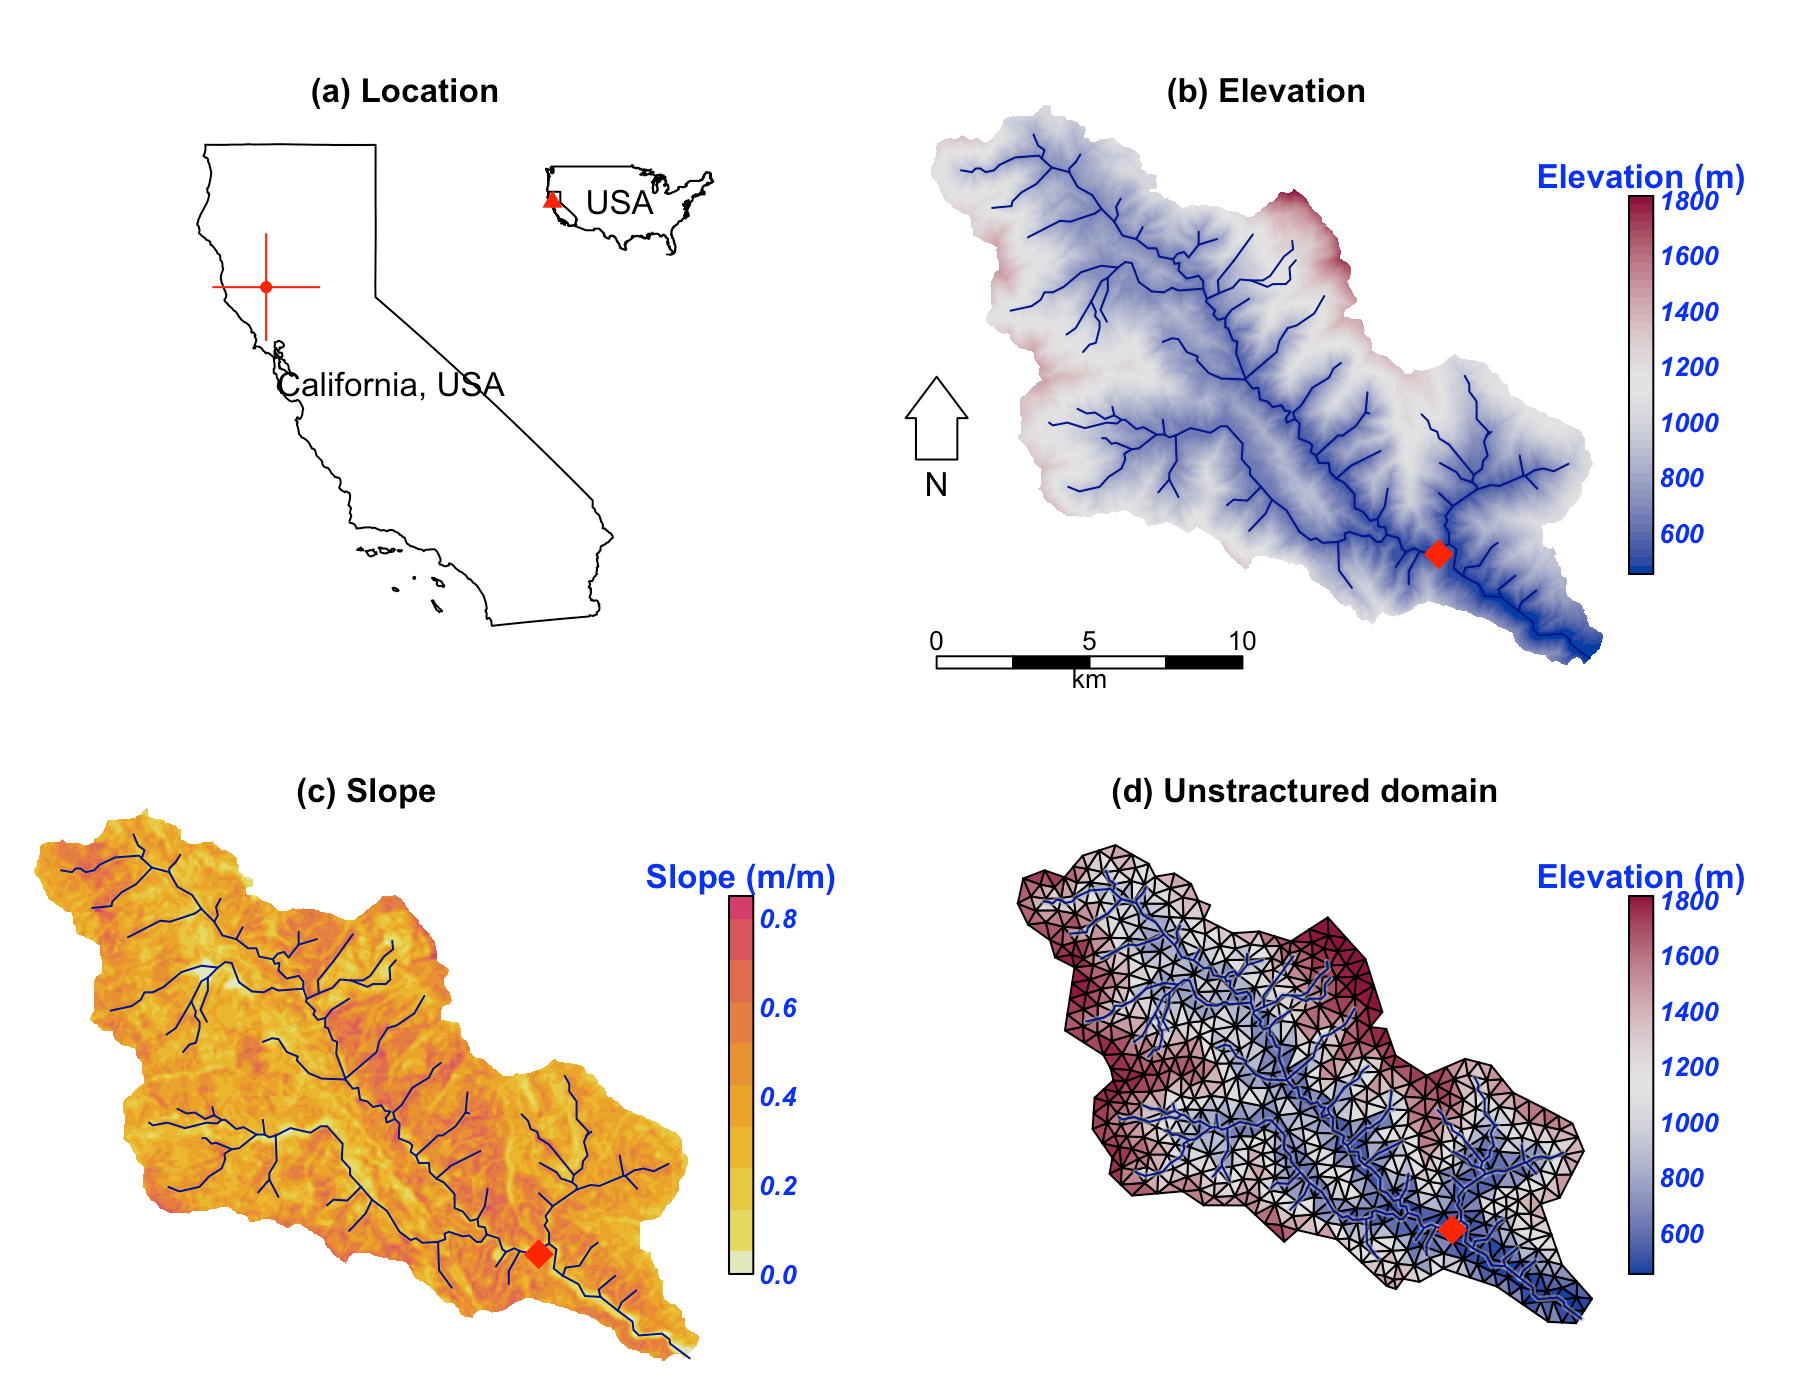
\includegraphics{Fig/Example/CacheCreek/sac5_map.png}
\caption{Location and data for Cache Creek Watershed}
\end{figure}

According to NLDAS-2, between 2000 and 2017 the mean temperature and
precipitation was \(12.8 ^\circ C\) and \(\approx 817 mm\),
respectively, in this catchment. Precipitation is unevenly distributed
through the year, with winter and spring precipitation being the vast
majority of the contribution to the annual total (Fig. \ref{fig:sh_pt}.

\begin{figure}
\centering
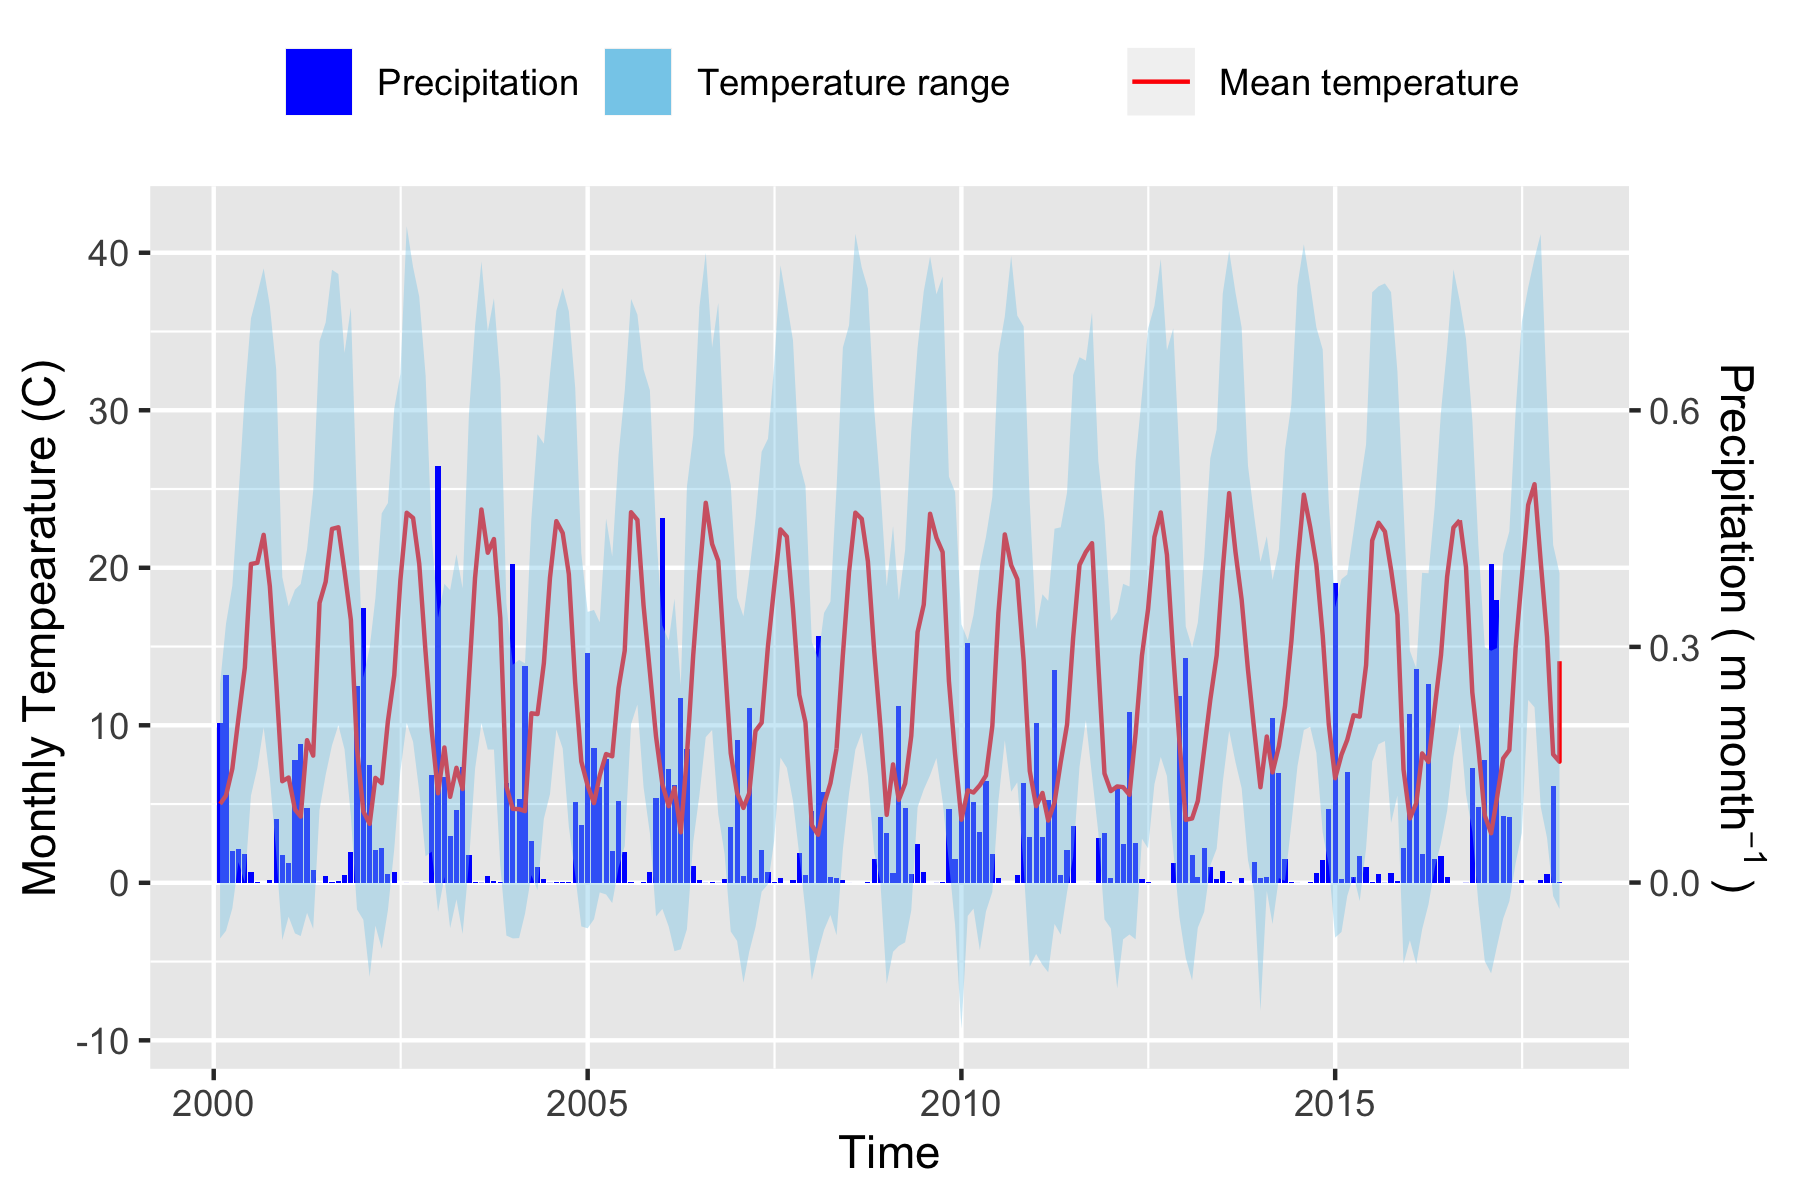
\includegraphics{Fig/Example/CacheCreek/sac5_PT.png}
\caption{Precipitation and temperature}
\end{figure}

\subsection{SHUD simulation and
calibration}\label{shud-simulation-and-calibration}

Our simulation in CCW covers the period from 2000 to 2007. Because of
the Mediterranean climate in this region, the simulation starts in
summer to ensure adequate time before the October start to the water
year. In our experiment, the first year (2000-06-01 to 2001-06-30) is
the spin-up period, the following two years (2001-07-01 to 2003-06-30 )
are the calibration period, and the period from 2003-07-01 to 2007-07-01
is for validation.

The unstructured domain of the CCW (Fig. \ref{fig:sh} (d)) is built with
SHUDtoolbox, a R package on GitHub
(\href{https://github.com/shud-system/SHUDtoolbox}{SHUDtoolbox}). The
number of triangular cells is 1147, with a mean area of \$ 0.17
km\^{}2\$. The total length of the river network is \(126.5 km\) and
consists of 103 river reaches and in which the highest order of stream
is 4. With a calibrated parameter set, the SHUD model tooks 5 hours to
simulate 17 years in the CCW, with a non-parallel configuration (OpenMP
is disabled on \emph{Mac Pro 2013 Xeon 2.7GHz, 32GB RAM}).

\subsection{Results}\label{results}

Figure \ref{fig:sh_calib} reveals the comparison of simulated discharge
against the observed discharge at the gage station of
\href{https://waterdata.usgs.gov/ca/nwis/uv/?site_no=11451100}{USGS
11451100}. The calibration procedure exploits the Covariance Matrix
Adaptation -- Evolution Strategy (CMA-ES) to calibrate automatically
\citep{Hansen2016}. The calibration program assigns 72 children in each
generation and keeps the best child as the seed for next-generation,
with limited perturbations. The perturbation for the next generation is
generated from the covariance matrix of the previous generation. After
23 generations, the calibration tool identifies a locally optimal
parameter set.

\begin{figure}
\centering
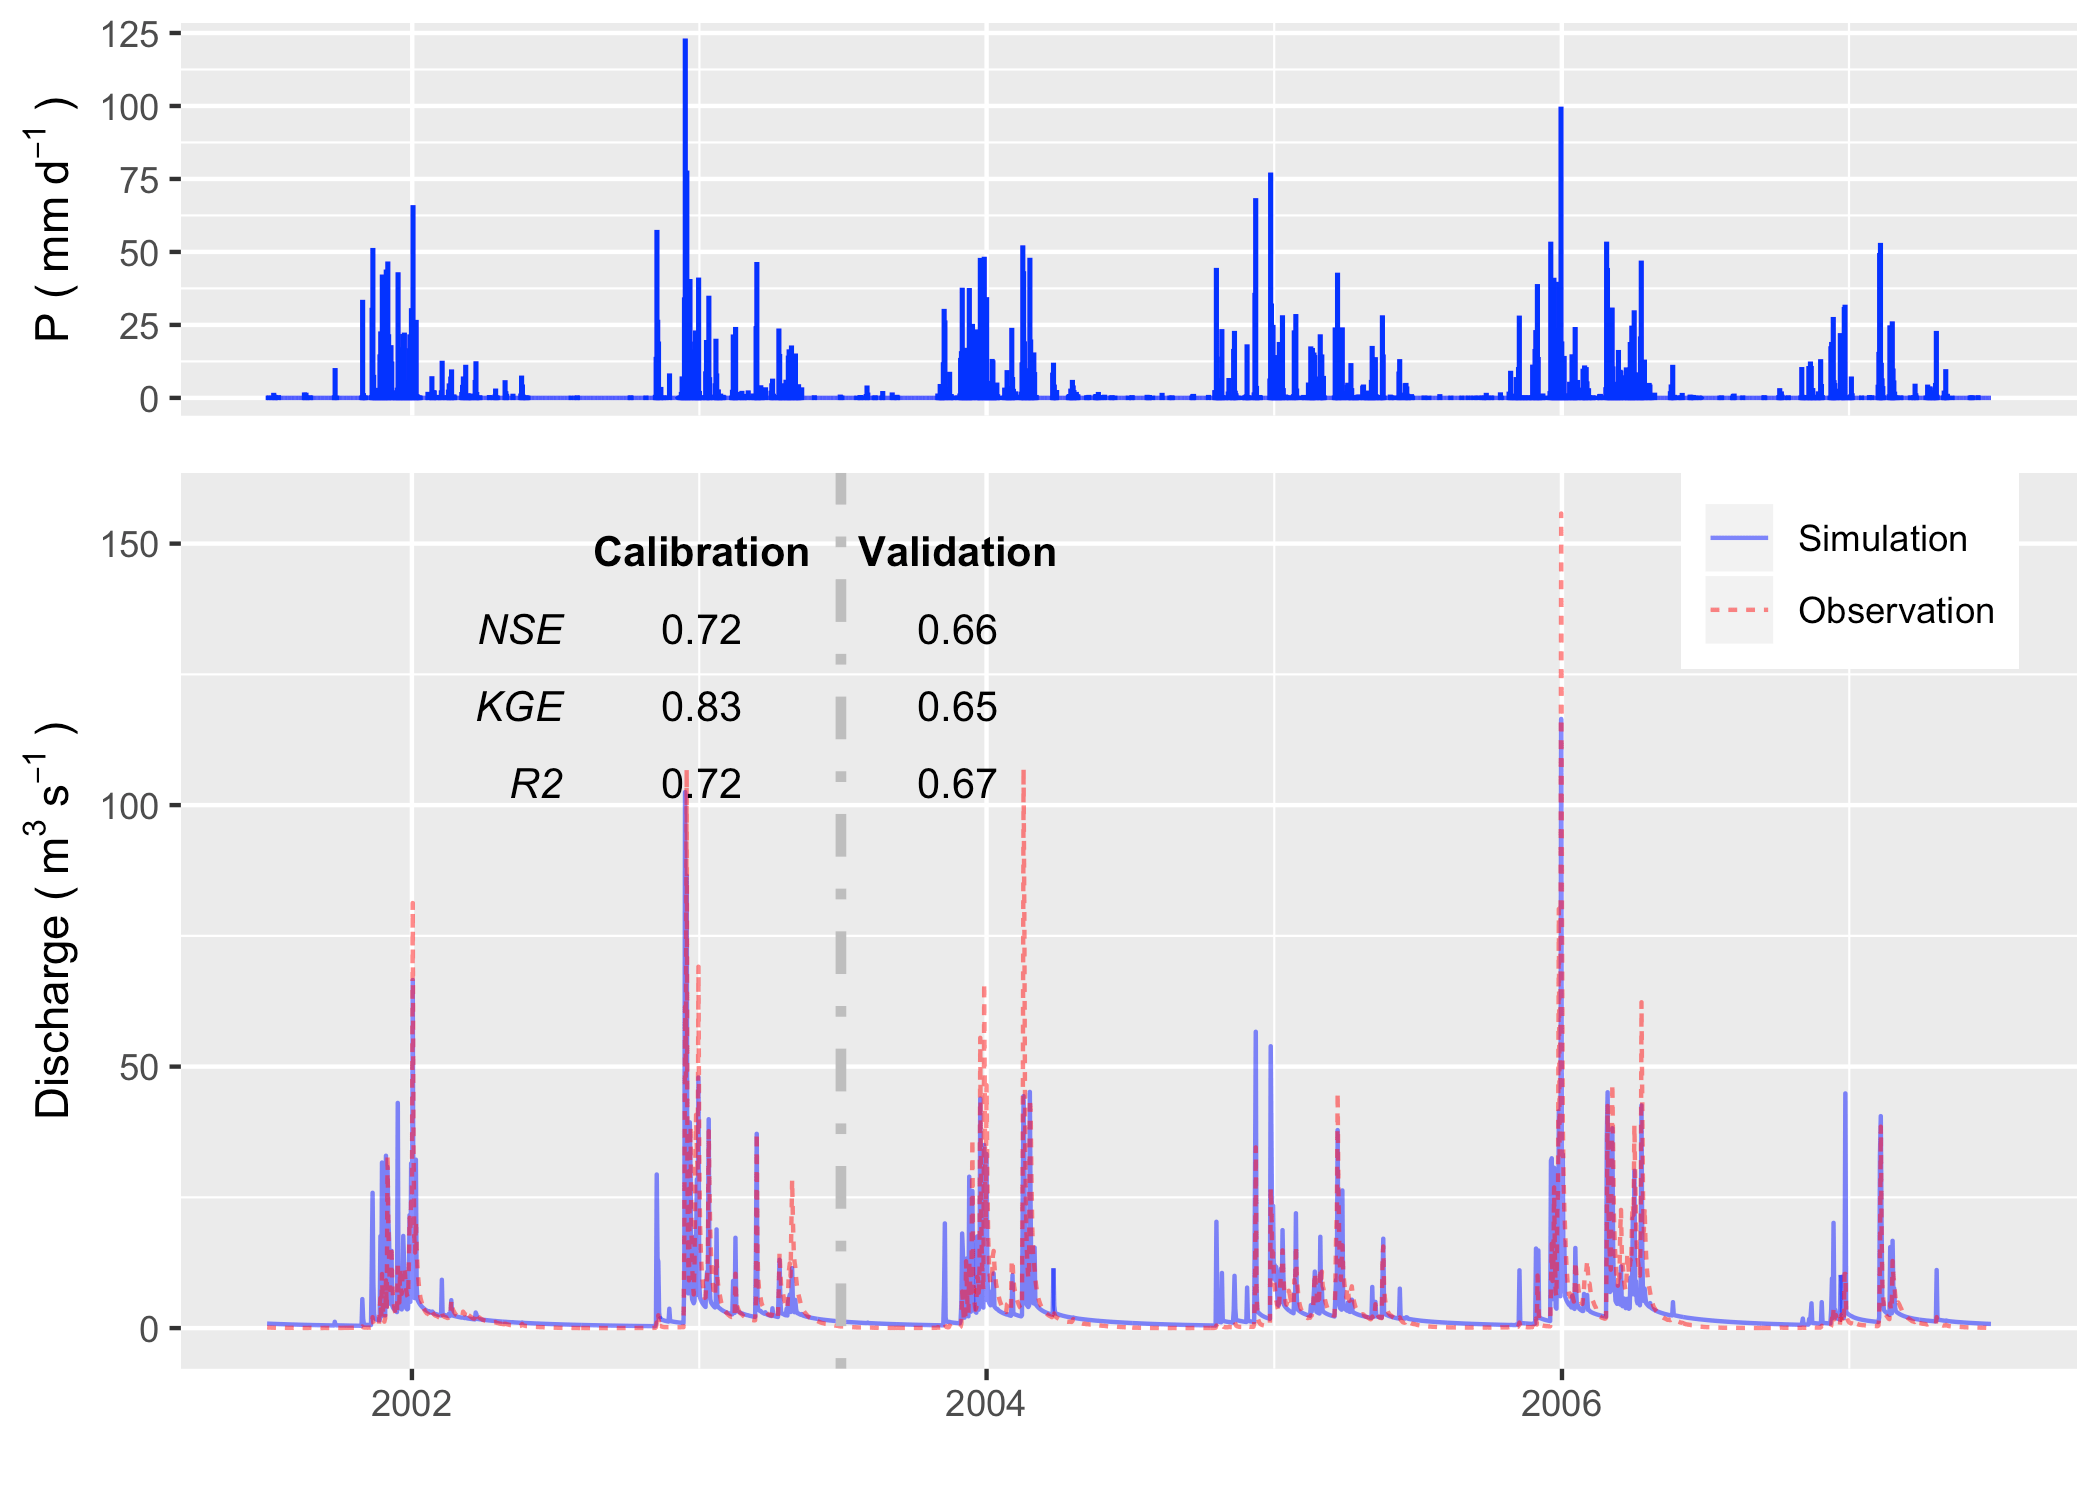
\includegraphics{Fig/Example/CacheCreek/sac5_hydrograph_daily.png}
\caption{The hydrograph in calibration and validation period}
\end{figure}

We use the groundwater distribution (Fig. \ref{fig:sh_gw}) to
demonstrate the spatial distribution of hydroligcal metrics calculated
from the SHUD model.

Figure \ref{fig:sh_gw} illustrates the annual mean groundwater table in
the validation period. Because the model fixes a \(30 m\) aquifer, the
results represent the groundwater within this aquifer only. The
groundwater table and elevation along the green line on the upper map
are extracted and plotted in the bottom figure. The gray ribbon is the
\(30 m\) aquifer, and the blue line is the location where groundwater
storage is larger than zero. The green polygons with the right axis are
the groundwater storage along the cross-section. The groundwater follows
the terrain, with groundwater accumulated in the valley, or along
relatively flat plains. In the CCW, the groundwater is very deep or does
not stay on the steep slope.

\begin{figure}
\centering
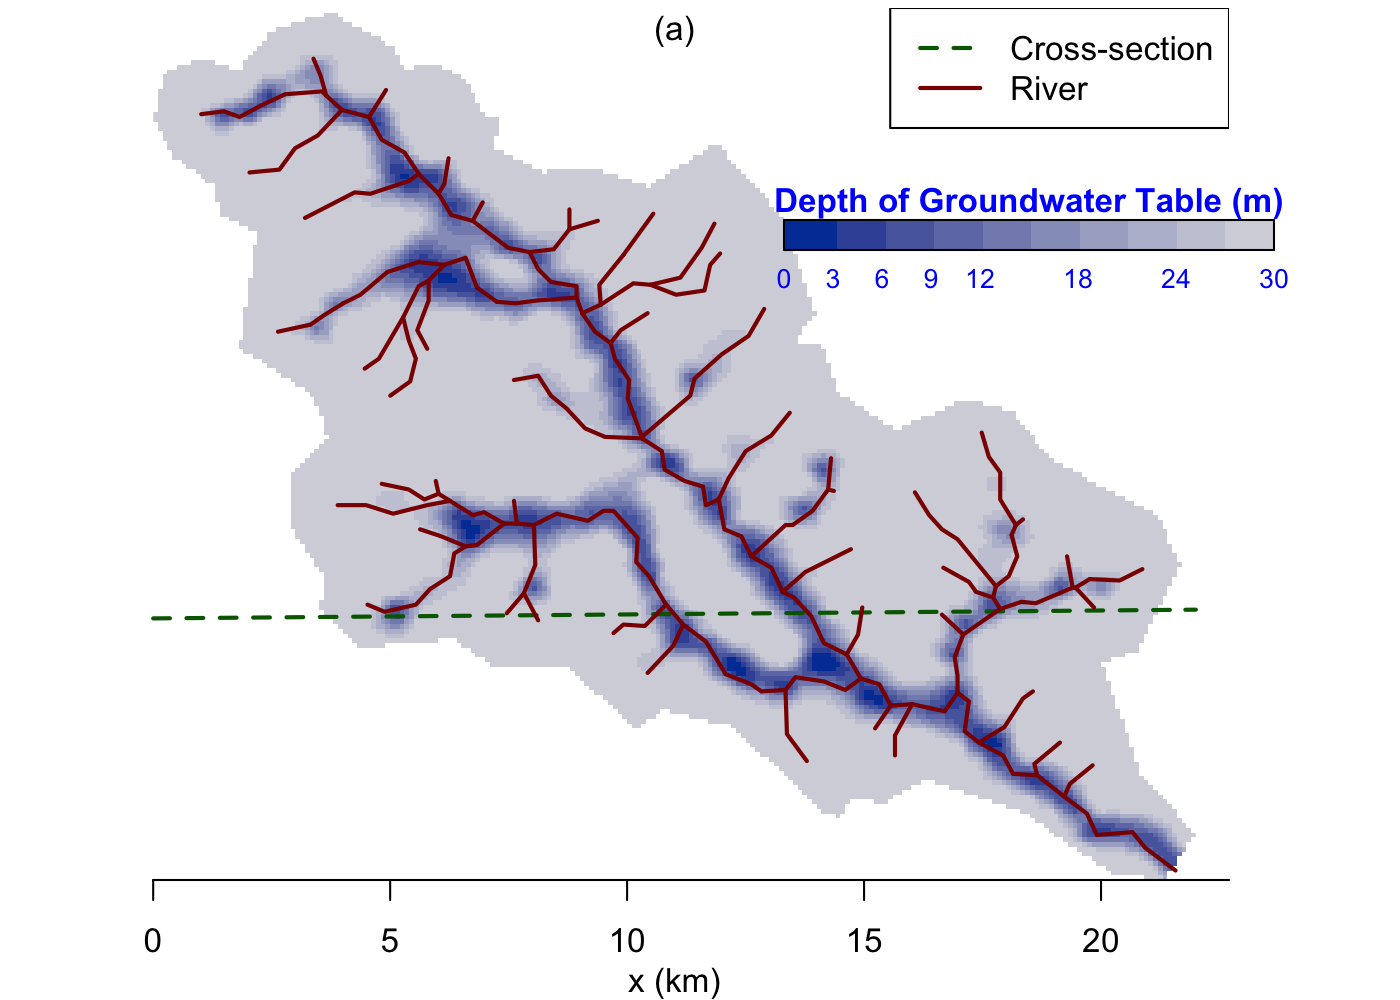
\includegraphics{Fig/Example/CacheCreek/sac5_rgw.png}
\caption{Groundwater spatial distribution map}
\end{figure}

\begin{figure}
\centering
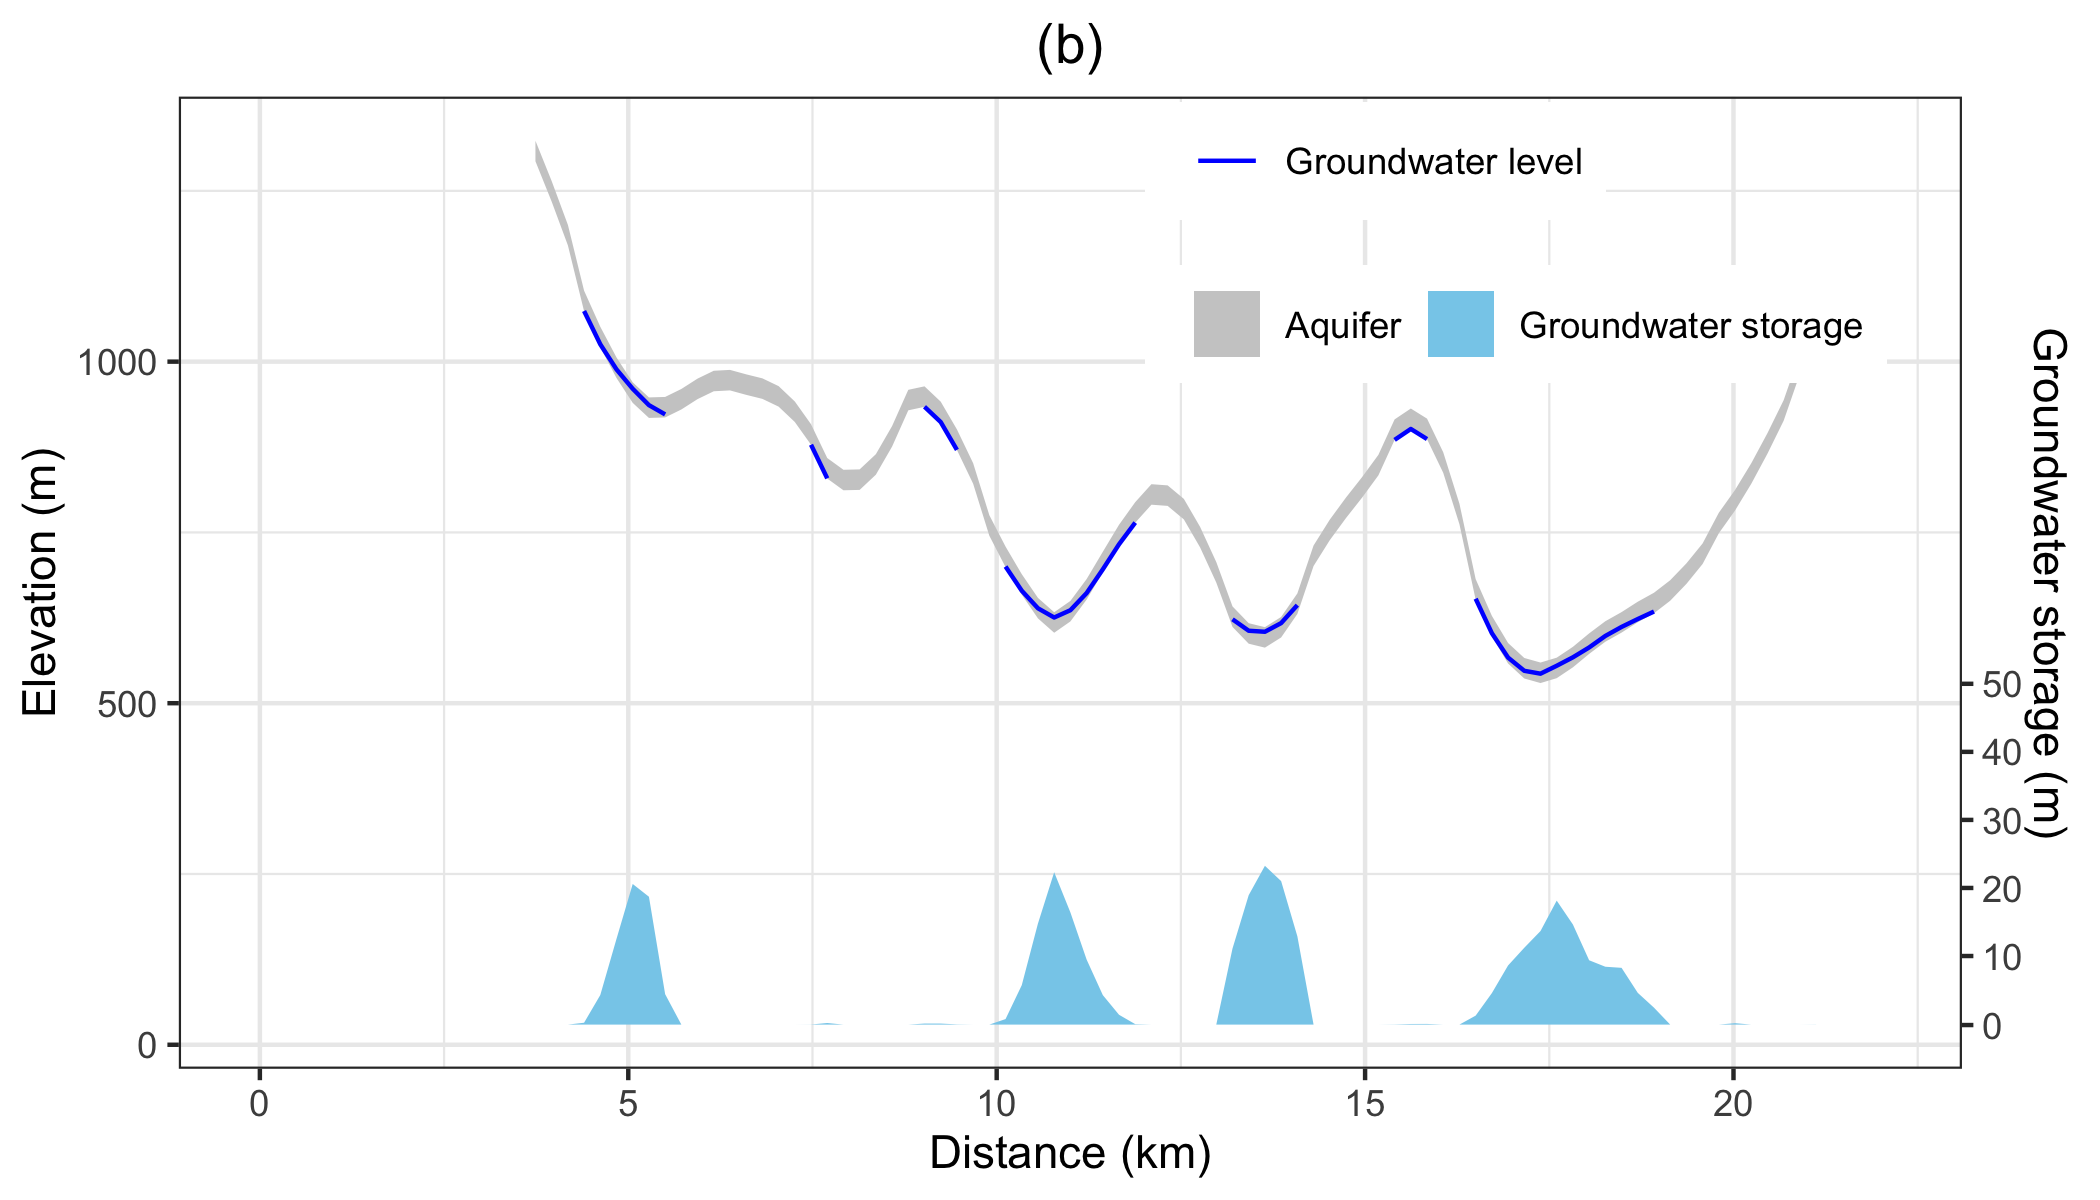
\includegraphics{Fig/Example/CacheCreek/sac5_sgw.png}
\caption{The groundwater condition along the cross-section line}
\end{figure}

\begin{figure}
\centering
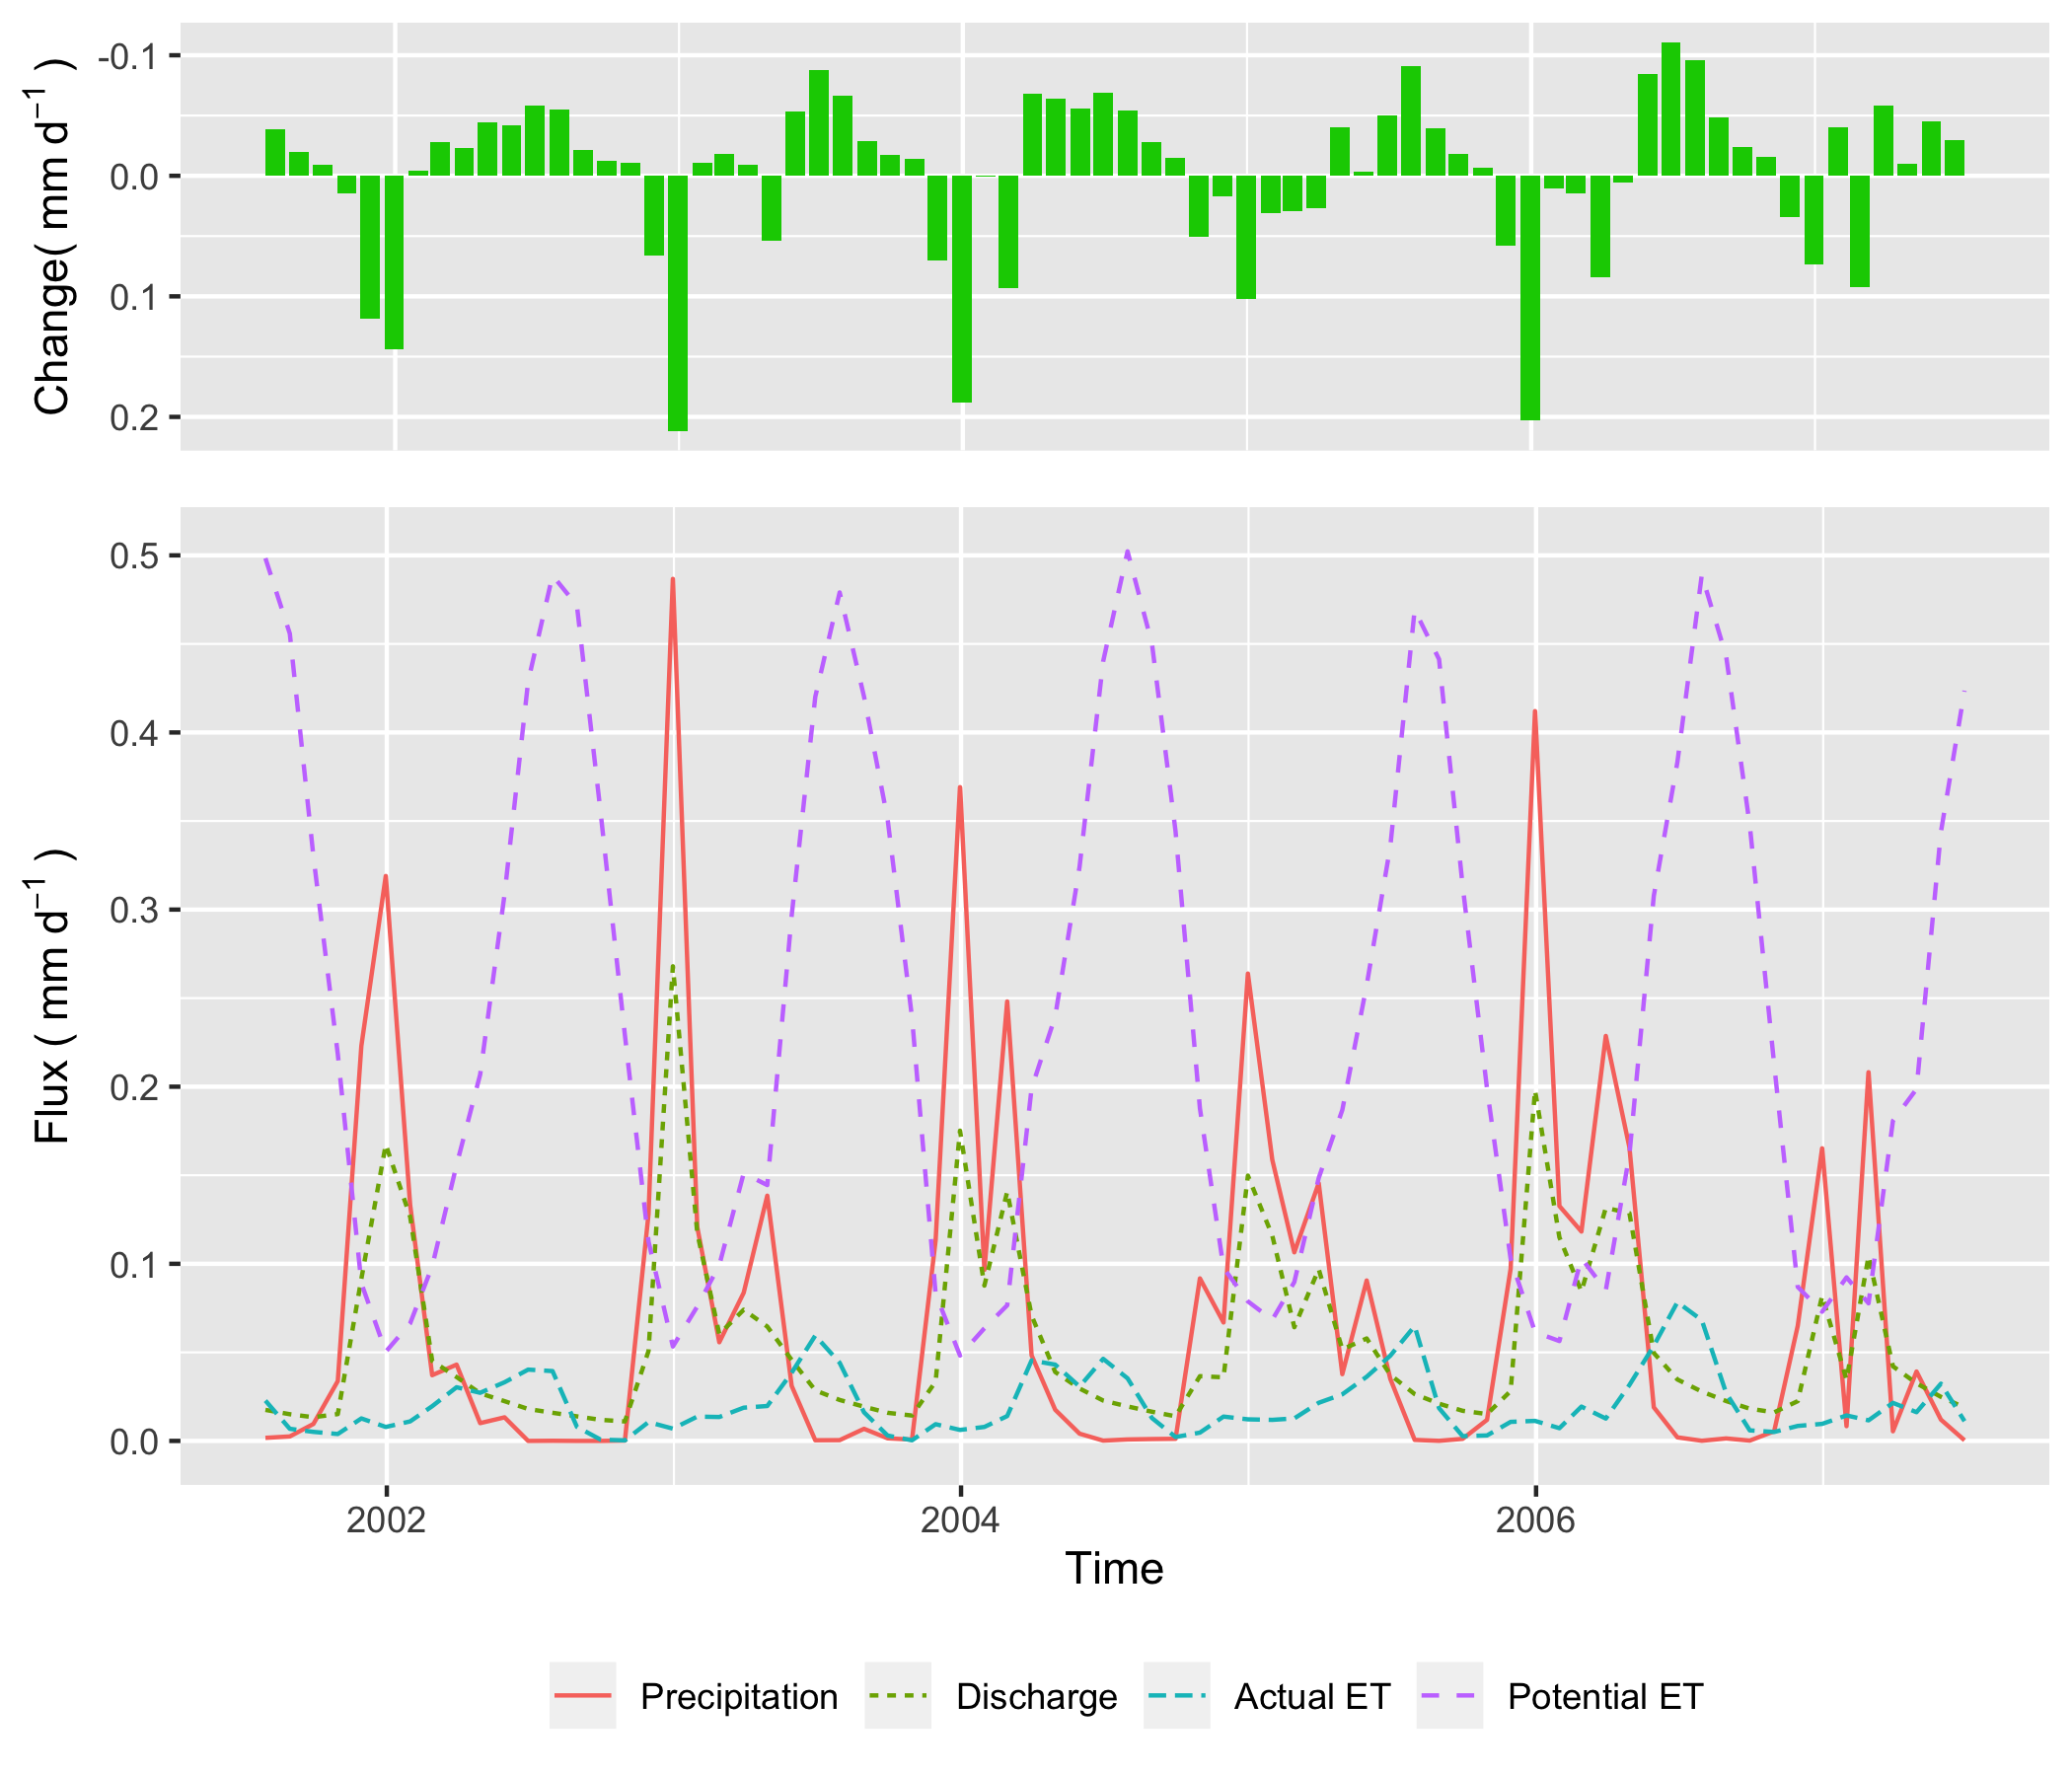
\includegraphics{Fig/Example/CacheCreek/sac5_wb.png}
\caption{Water balance in the simulation period}
\end{figure}

\section{Example 4: Flashy flood in Yanhua Village, Ningxia, China on
September
2018}\label{example-4-flashy-flood-in-yanhua-village-ningxia-china-on-september-2018}

\begin{figure}
\centering
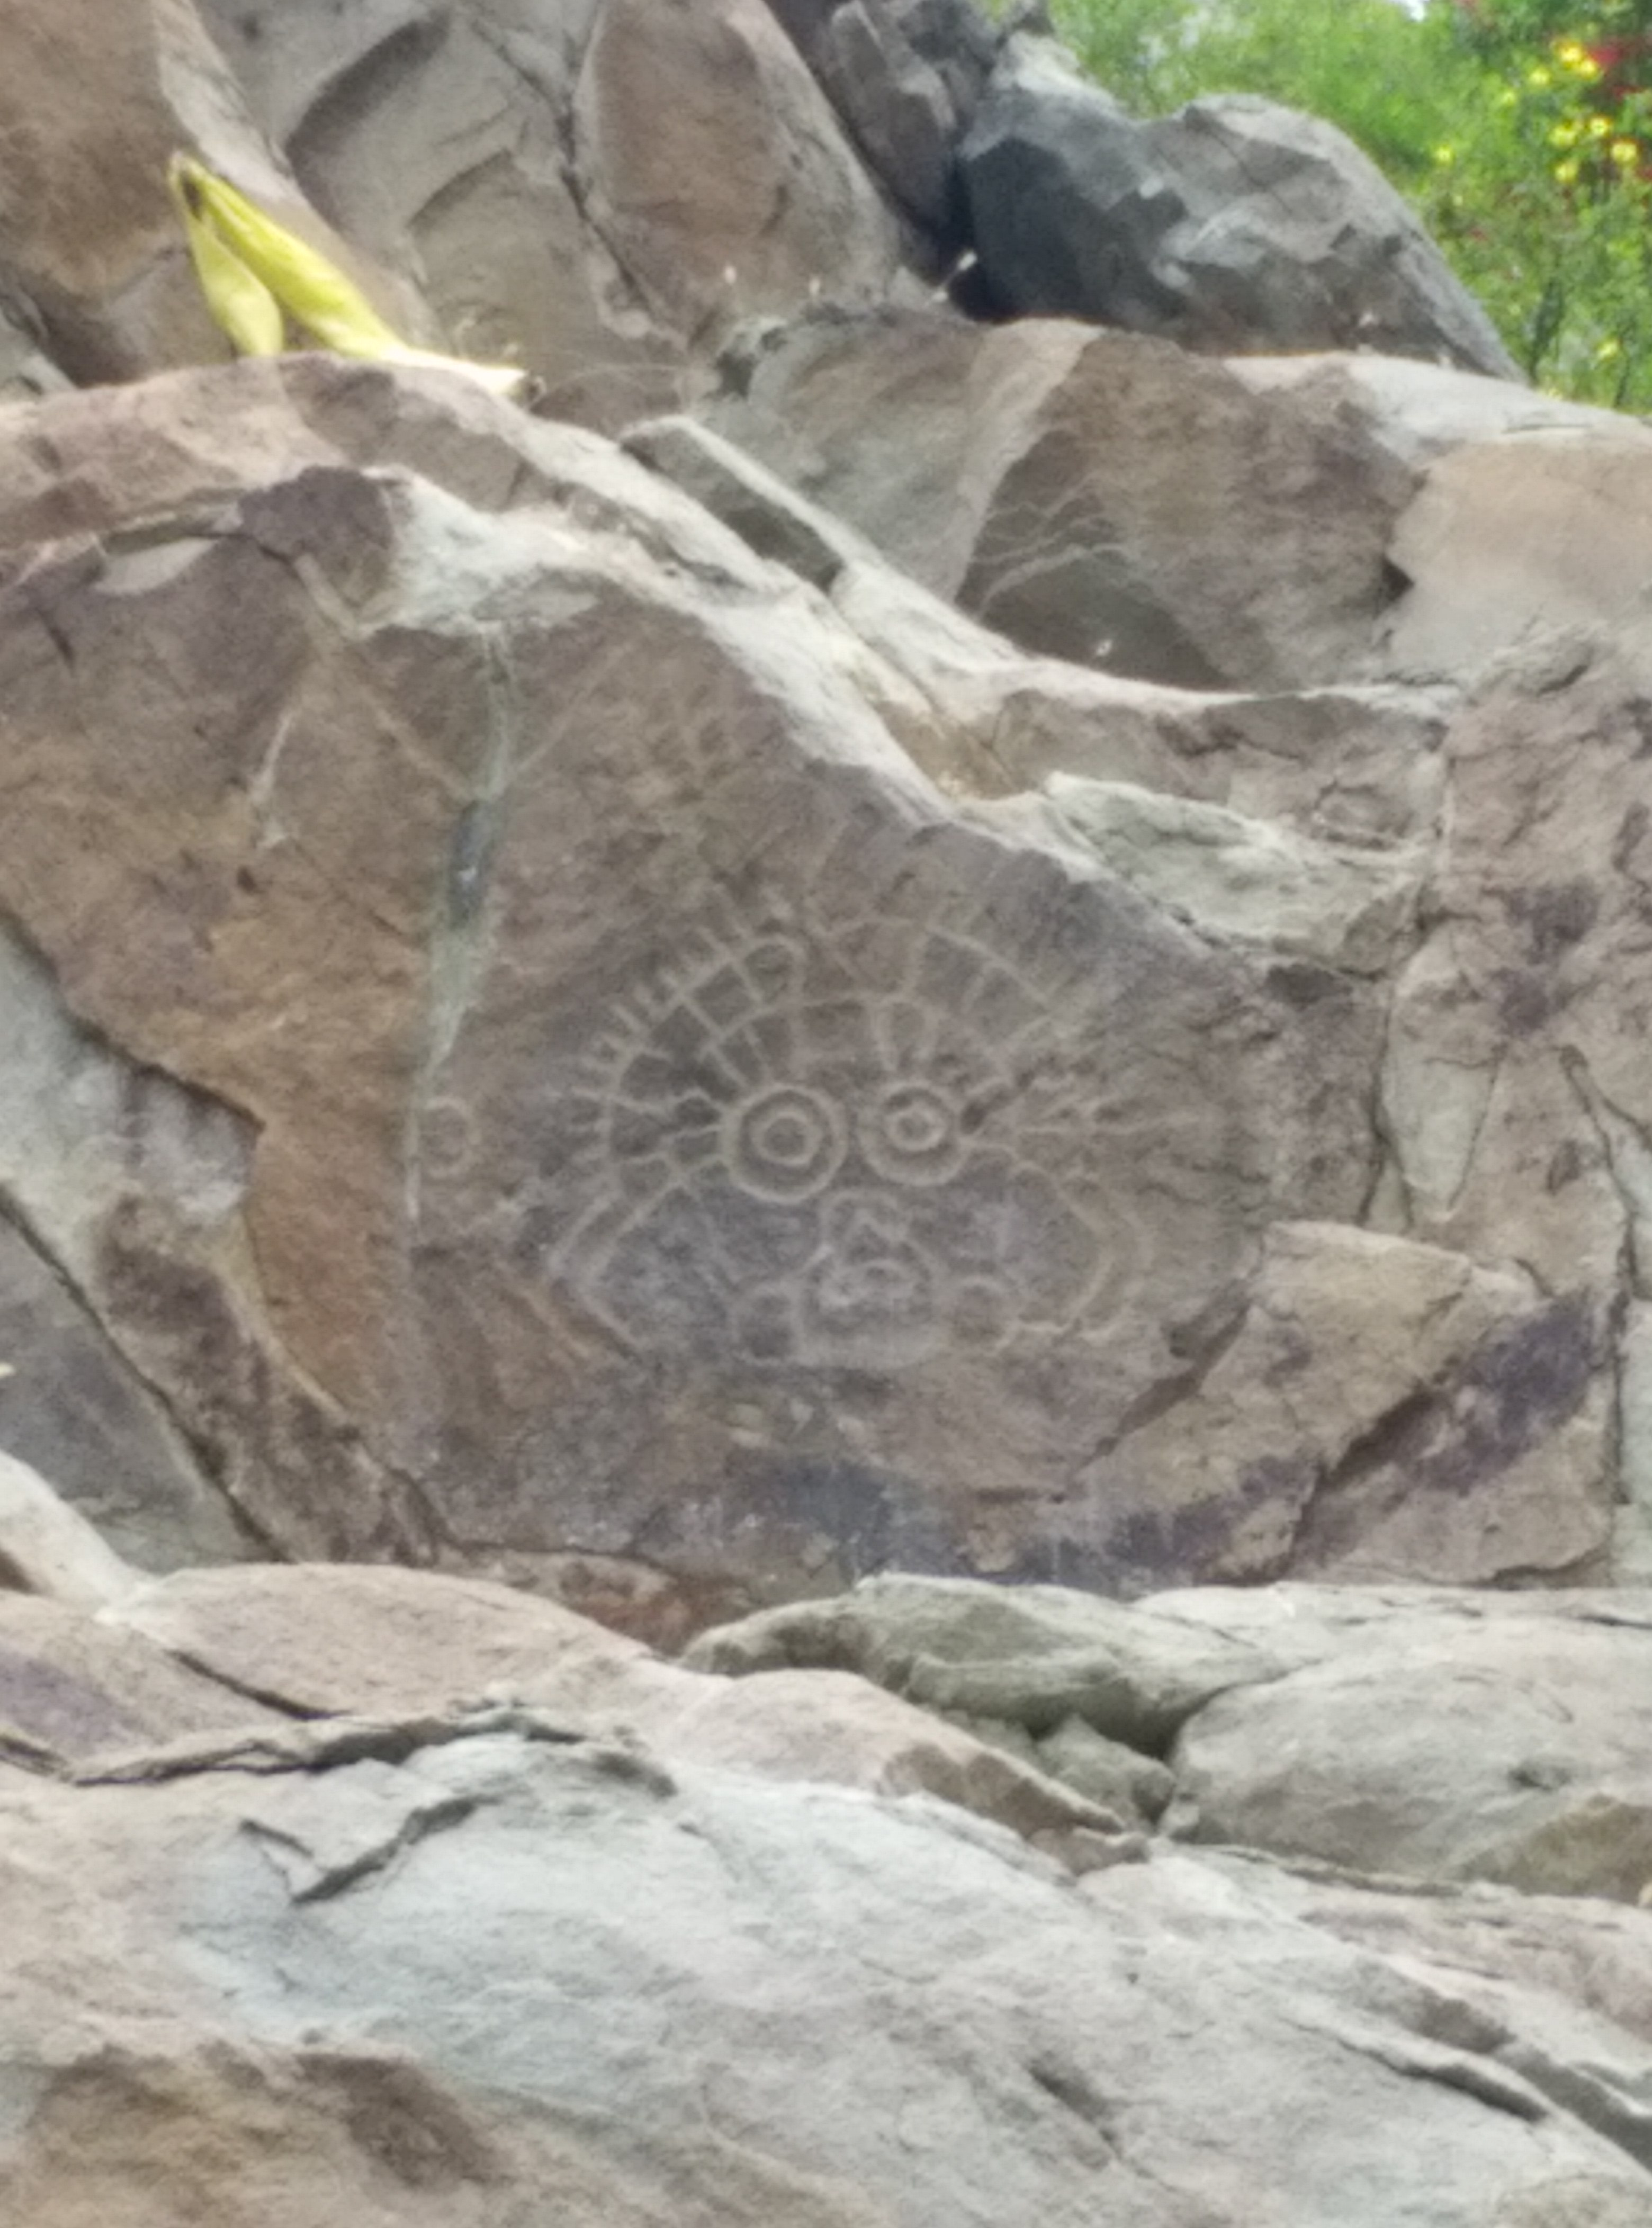
\includegraphics{Fig/Example/Yanhuacun/sun.jpg}
\caption{The Sun God of Perietal Art (Source: wiki)}
\end{figure}

\begin{figure}
\centering
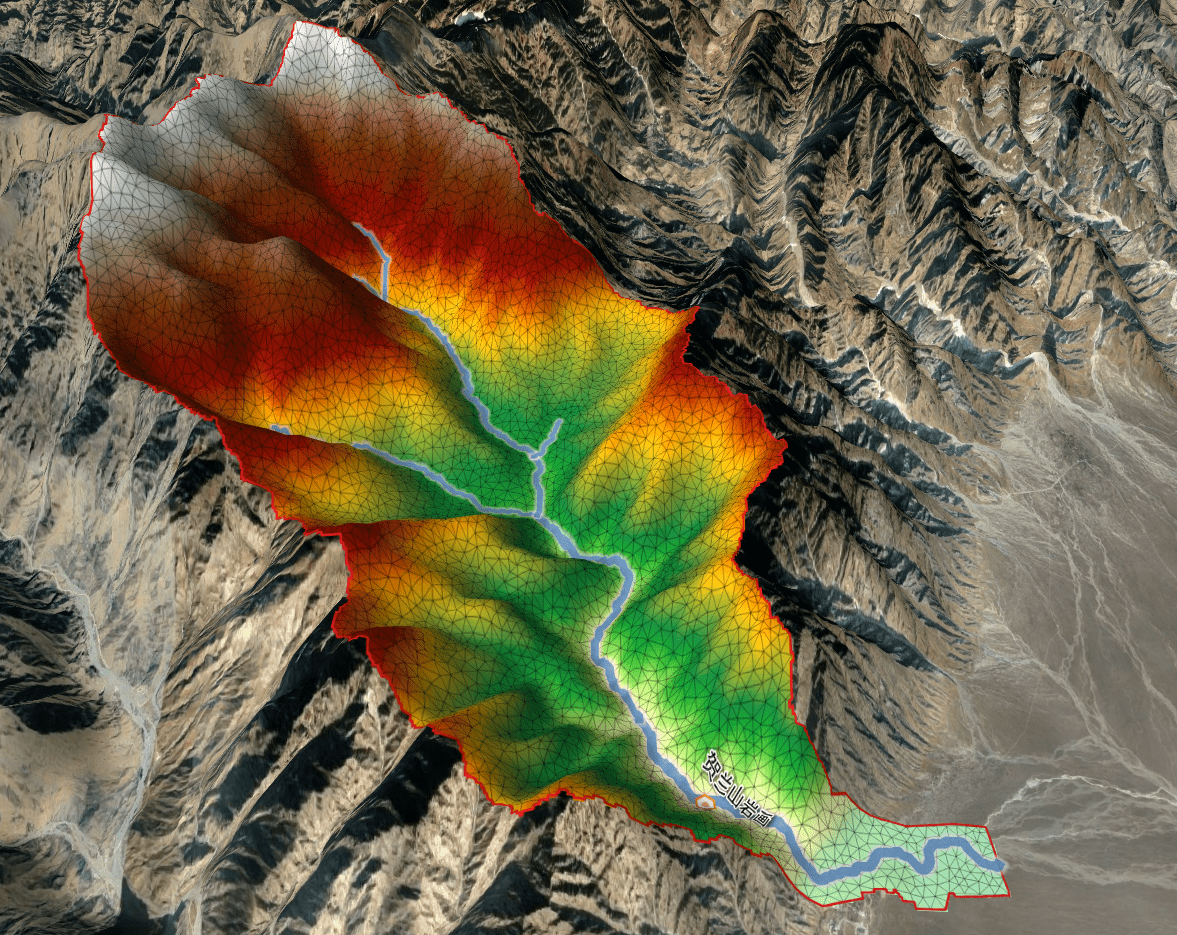
\includegraphics{Fig/Example/Yanhuacun/map.png}
\caption{Triangular modeling domain of the Yanhua Village)}
\end{figure}

\section{Example 5: Flood inundation in Houston during Harvey Hurricane
2017}\label{example-5-flood-inundation-in-houston-during-harvey-hurricane-2017}

\section{Example 6: Watershed in South
Sudan}\label{example-6-watershed-in-south-sudan}

\chapter{Calibration}\label{calibration}

\emph{This chapter is imcomplete}

\begin{longtable}[]{@{}cccc@{}}
\toprule
File & Comments & Header & \# of column\tabularnewline
\midrule
\endhead
.cfg.cmaes & Configuration of CMA-ES method & No & -\tabularnewline
\bottomrule
\end{longtable}

Values in .calib.cmaes file:

\begin{longtable}[]{@{}ccccc@{}}
\toprule
Item & Meaning & Default value & Range & Unit\tabularnewline
\midrule
\endhead
lambda & Number of children in each generation & 48 & & -\tabularnewline
stopfitness & Threshold to accept the \emph{best} solution & 0.3 & &
-\tabularnewline
maxgen & Maximun generations & 48 & & -\tabularnewline
sigma & & 0.8 & & -\tabularnewline
updateic & Whether to update initial condition after each generation & 0
& 0/1 & -\tabularnewline
walltime & Walltime to kill the modeling thread & 86400 & 0-inf &
second\tabularnewline
nspingup & Number of days for spinup & 0 & 0-inf & day\tabularnewline
& & & & -\tabularnewline
\bottomrule
\end{longtable}

Values in .calib.range file:

Rows: Values in .cfg.calib file. Column: \textbar{} Item \textbar{}
Meaning \textbar{} Default value \textbar{} Range \textbar{} Unit
\textbar{}
\textbar{}:------:\textbar{}:--------------------------:\textbar{}:---------:\textbar{}:---------:\textbar{}:--------:\textbar{}
\textbar{} On/off \textbar{} On or Off \textbar{} 0 \textbar{} 0/1
\textbar{} - \textbar{} \textbar{} log \textbar{} Whether logrithm
\textbar{} 0 \textbar{} 0/1 \textbar{} - \textbar{} \textbar{} min
\textbar{} Minimun value \textbar{} - \textbar{} - \textbar{} -
\textbar{} \textbar{} max \textbar{} Maximun value \textbar{} -
\textbar{} - \textbar{} - \textbar{}

\chapter{Quick, Reproducible and Automatic hydrological
modeling}\label{quick-reproducible-and-automatic-hydrological-modeling}

\section{Steps of modeling with SHUD}\label{steps-of-modeling-with-shud}

\subsection{Essential Terrestrial
Variables?}\label{essential-terrestrial-variables}

\begin{itemize}
\tightlist
\item
  Atmospheric forcing (precipitation, snow cover, wind, relative
  humidity, temperature, net radiation, albedo, photosynthetic
  atmospheric radiation, leaf area index)
\item
  Digital elevation model (DEM)
\item
  River/stream discharge
\item
  Soil (class, hydrologic properties)
\item
  Groundwater (levels, extent, hydro-geologic properties)
\item
  Lake/Reservoir (levels, extent)
\item
  Land cover and land use (biomass, human infrastructure, demography,
  ecosystem disturbance)
\item
  Water use
\end{itemize}

Most data reside on federal servers \ldots{}.many petabytes.

\subsection{A-Priori Data Sources}\label{a-priori-data-sources}

\begin{longtable}[]{@{}ccc@{}}
\toprule
\begin{minipage}[b]{0.11\columnwidth}\centering\strut
Feature/Time-Series\strut
\end{minipage} & \begin{minipage}[b]{0.19\columnwidth}\centering\strut
Property\strut
\end{minipage} & \begin{minipage}[b]{0.42\columnwidth}\centering\strut
Source\strut
\end{minipage}\tabularnewline
\midrule
\endhead
\begin{minipage}[t]{0.11\columnwidth}\centering\strut
Soil\strut
\end{minipage} & \begin{minipage}[t]{0.19\columnwidth}\centering\strut
Porosity; Sand, Silt, Clay Fractions; Bulk Density\strut
\end{minipage} & \begin{minipage}[t]{0.42\columnwidth}\centering\strut
CONUS, SSURGO and STATSGO\strut
\end{minipage}\tabularnewline
\begin{minipage}[t]{0.11\columnwidth}\centering\strut
Geology\strut
\end{minipage} & \begin{minipage}[t]{0.19\columnwidth}\centering\strut
Bed Rock Depth; Horizontal and Vertical Hydraulic Conductivity\strut
\end{minipage} & \begin{minipage}[t]{0.42\columnwidth}\centering\strut
\url{http://www.dcnr.state.pa.us/topogeo/},
\url{http://www.lias.psu.edu/emsl/guides/X.html}\strut
\end{minipage}\tabularnewline
\begin{minipage}[t]{0.11\columnwidth}\centering\strut
Land Cover\strut
\end{minipage} & \begin{minipage}[t]{0.19\columnwidth}\centering\strut
LAI\strut
\end{minipage} & \begin{minipage}[t]{0.42\columnwidth}\centering\strut
\href{http://glcf.umiacs.umd.edu/data/landcover/data.shtml}{UMC},
\href{http://ldas.gsfc.nasa.gov/LDAS8th/MAPPED.VEG/LDASmapveg.shtml}{LDASmapveg};\strut
\end{minipage}\tabularnewline
\begin{minipage}[t]{0.11\columnwidth}\centering\strut
Land Cover\strut
\end{minipage} & \begin{minipage}[t]{0.19\columnwidth}\centering\strut
Manning's Roughness;\strut
\end{minipage} & \begin{minipage}[t]{0.42\columnwidth}\centering\strut
Hernandez et. al., 2000\strut
\end{minipage}\tabularnewline
\begin{minipage}[t]{0.11\columnwidth}\centering\strut
River\strut
\end{minipage} & \begin{minipage}[t]{0.19\columnwidth}\centering\strut
Manning's Roughness;\strut
\end{minipage} & \begin{minipage}[t]{0.42\columnwidth}\centering\strut
Dingman (2002)\strut
\end{minipage}\tabularnewline
\begin{minipage}[t]{0.11\columnwidth}\centering\strut
River\strut
\end{minipage} & \begin{minipage}[t]{0.19\columnwidth}\centering\strut
Coefficient of Discharge\strut
\end{minipage} & \begin{minipage}[t]{0.42\columnwidth}\centering\strut
ModHms Manual (Panday and Huyakorn, 2004)\strut
\end{minipage}\tabularnewline
\begin{minipage}[t]{0.11\columnwidth}\centering\strut
River\strut
\end{minipage} & \begin{minipage}[t]{0.19\columnwidth}\centering\strut
Shape and Dimensions;\strut
\end{minipage} & \begin{minipage}[t]{0.42\columnwidth}\centering\strut
Derived from regression using depth, width, and discharge data from
\href{http://nwis.waterdata.usgs.gov/usa/nwis/measurements}{USGS
data}\strut
\end{minipage}\tabularnewline
\begin{minipage}[t]{0.11\columnwidth}\centering\strut
River\strut
\end{minipage} & \begin{minipage}[t]{0.19\columnwidth}\centering\strut
Topology: Nodes, Neighboring cells;\strut
\end{minipage} & \begin{minipage}[t]{0.42\columnwidth}\centering\strut
Derived using PIHMgis (Bhatt et. al., 2008)\strut
\end{minipage}\tabularnewline
\begin{minipage}[t]{0.11\columnwidth}\centering\strut
Forcing\strut
\end{minipage} & \begin{minipage}[t]{0.19\columnwidth}\centering\strut
Prec, Temp. RH, Wind, Rad.\strut
\end{minipage} & \begin{minipage}[t]{0.42\columnwidth}\centering\strut
National Land Data Assimilation System: NLDAS-2\strut
\end{minipage}\tabularnewline
\begin{minipage}[t]{0.11\columnwidth}\centering\strut
Topography\strut
\end{minipage} & \begin{minipage}[t]{0.19\columnwidth}\centering\strut
DEM\strut
\end{minipage} & \begin{minipage}[t]{0.42\columnwidth}\centering\strut
\url{http://seamless.usgs.gov/}\strut
\end{minipage}\tabularnewline
\begin{minipage}[t]{0.11\columnwidth}\centering\strut
Streamflow\strut
\end{minipage} & \begin{minipage}[t]{0.19\columnwidth}\centering\strut
\strut
\end{minipage} & \begin{minipage}[t]{0.42\columnwidth}\centering\strut
\url{http://nwis.waterdata.usgs.gov/nwis/sw}\strut
\end{minipage}\tabularnewline
\begin{minipage}[t]{0.11\columnwidth}\centering\strut
Groundwater\strut
\end{minipage} & \begin{minipage}[t]{0.19\columnwidth}\centering\strut
\strut
\end{minipage} & \begin{minipage}[t]{0.42\columnwidth}\centering\strut
\url{http://nwis.waterdata.usgs.gov/nwis/gw}\strut
\end{minipage}\tabularnewline
\bottomrule
\end{longtable}

\section{Workflow of SHUD Modeling
System}\label{workflow-of-shud-modeling-system}

\begin{enumerate}
\def\labelenumi{\arabic{enumi}.}
\tightlist
\item
  Prepare raw Essential Terrestrial Variables (ETV)
\item
  Convert and crop raw data with the research area boundary.
\item
  Build the unstructued modeling domain with
  \href{https://github.com/SHUD-System/SHUD}{SHUDboolbox}
\item
  Run SHUD on desktop or cluster.
\item
  Analysis the SHUD model results with
  \href{https://github.com/SHUD-System/SHUDboolbox}{SHUDboolbox} or your
  hydrologic analysis tools.
\end{enumerate}

\begin{figure}
\centering
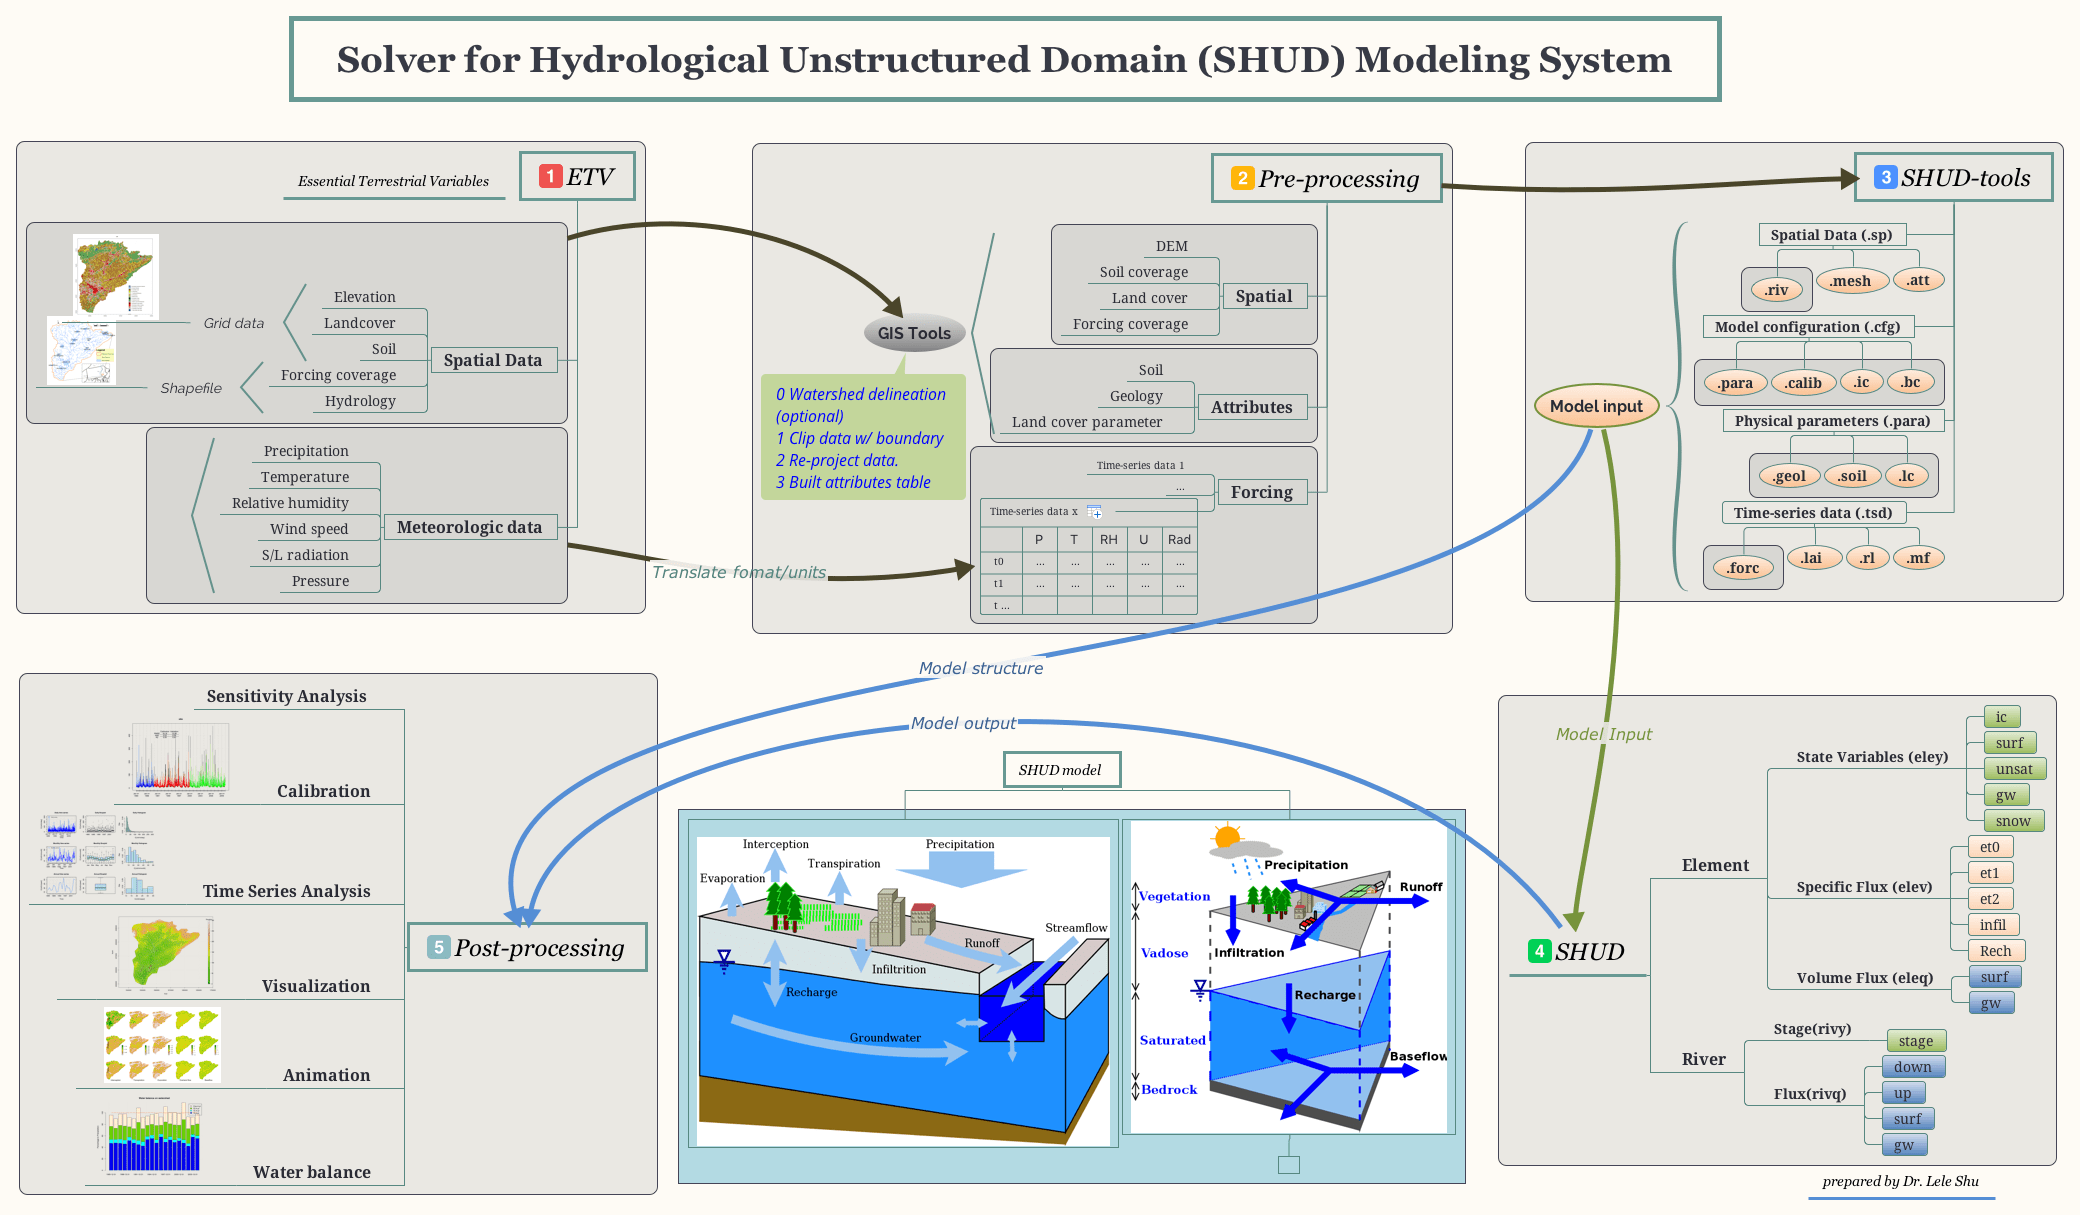
\includegraphics{./Fig/autoSHUD.png}
\caption{The workflow of modeling with SHUD Modeling System}
\end{figure}

\chapter{Source code and program
design}\label{source-code-and-program-design}

The source code of SHUD and SHUD-tool are avaliable via Github:
\url{https://github.com/SHUD-System/SHUD} and
\url{https://github.com/SHUD-System/SHUDtoolbox}.

\bibliography{book.bib}

\end{document}
